\documentclass[
  % -- opções da classe memoir --
  12pt,       % tamanho da fonte
  % openright,      % capítulos começam em pág ímpar (insere página vazia caso preciso)
  oneside,      % para impressão em verso e anverso, use twoside.
  a4paper,      % tamanho do papel. 
  % -- opções da classe abntex2 --
  %chapter=TITLE,   % títulos de capítulos convertidos em letras maiúsculas
  %section=TITLE,   % títulos de seções convertidos em letras maiúsculas
  %subsection=TITLE,  % títulos de subseções convertidos em letras maiúsculas
  %subsubsection=TITLE,% títulos de subsubseções convertidos em letras maiúsculas
  % -- opções do pacote babel --
  english,      % idioma adicional para hifenização
  %french,       % idioma adicional para hifenização
  %spanish,      % idioma adicional para hifenização
  brazil        % o último idioma é o principal do documento
  ]{abntex2}

% ---
% Pacotes básicos 
% ---
\usepackage{lmodern}      % Usa a fonte Latin Modern      
\usepackage[T1]{fontenc}    % Selecao de codigos de fonte.
\usepackage[utf8]{inputenc}   % Codificacao do documento (conversão automática dos acentos)
\usepackage{lastpage}     % Usado pela Ficha catalográfica
\usepackage{indentfirst}    % Indenta o primeiro parágrafo de cada seção.
\usepackage{color}        % Controle das cores
\usepackage{graphicx}     % Inclusão de gráficos
\usepackage{microtype}      % para melhorias de justificação
\usepackage{amsmath}      % para fórmulas matemáticas
\usepackage{amssymb}      % para símbolos matemáticos
\usepackage{listings}     % para listagens de código
\usepackage{caption}      % para legendas
\usepackage{subcaption}   % para imagens aninhadas
\usepackage{multirow}     % para row span em tabelas
\usepackage[table,usenames,dvipsnames]{xcolor} % para cores especiais

% ---
% Pacotes de citações
% ---
\usepackage[brazilian,hyperpageref]{backref}   % Paginas com as citações na bibl
\usepackage[alf]{abntex2cite} % Citações padrão ABNT

% --- 
% CONFIGURAÇÕES DE PACOTES
% --- 

% ---
% Configurações do pacote backref
% Usado sem a opção hyperpageref de backref
\renewcommand{\backrefpagesname}{Citado na(s) página(s):~}
% Texto padrão antes do número das páginas
\renewcommand{\backref}{}
% Define os textos da citação
\renewcommand*{\backrefalt}[4]{
  \ifcase #1 %
    Nenhuma citação no texto.%
  \or
    Citado na página #2.%
  \else
    Citado #1 vezes nas páginas #2.%
  \fi}%
% ---
\renewcommand{\lstlistingname}{Listagem}
% ---
% Informações de dados para CAPA e FOLHA DE ROSTO
% ---
\titulo{Processo para Inferência de Desempenho de \\ Configurações para Execução de Aplicações em \\ Ambientes de Nuvem de Infraestrutura}
\autor{Marcelo Canário Gonçalves}
\orientador{Prof. Dr. Américo Tadeu Falcone Sampaio}
\coorientador{Prof. Dr. Nabor das Chagas Mendonça}
\instituicao{%
  Universidade de Fortaleza
  \par
  Programa de Pós-Graduação em Informática Aplicada (PPGIA)}
\local{FORTALEZA}
\data{2014}
\tipotrabalho{Dissertação (Mestrado)}

% O preambulo deve conter o tipo do trabalho, o objetivo, 
% o nome da instituição e a área de concentração 
\preambulo{Dissertação apresentada ao Programa de Pós-Graduação em Informática
Aplicada (PPGIA) da Universidade de Fortaleza como parte dos requisitos
necessários para a obtenção do grau de Mestre em Informática Aplicada.}
% ---

% ---
% Configurações de aparência do PDF final

% alterando o aspecto da cor azul
\definecolor{blue}{RGB}{41,5,195}

% informações do PDF
\makeatletter
\hypersetup{
      %pagebackref=true,
    pdftitle={\@title}, 
    pdfauthor={\@author},
      pdfsubject={\imprimirpreambulo},
      pdfcreator={LaTeX with abnTeX2},
    pdfkeywords={abnt}{latex}{abntex}{abntex2}{trabalho acadêmico}, 
    %colorlinks=false,          % false: boxed links; true: colored links
      linkcolor=blue,           % color of internal links
      %citecolor=blue,           % color of links to bibliography
      filecolor=magenta,          % color of file links
    urlcolor=blue,
    bookmarksdepth=4
}
\makeatother
% --- 

% --- 
% Espaçamentos entre linhas e parágrafos 
% --- 

% O tamanho do parágrafo é dado por:
\setlength{\parindent}{1.3cm}

% Controle do espaçamento entre um parágrafo e outro:
\setlength{\parskip}{0.2cm}  % tente também \onelineskip

%Altera a capa
% Impressão da Capa
\renewcommand{\imprimircapa}{%
\begin{capa}%
\center

% Logomarca da Universidade

\includegraphics[scale=2]{./img/logo.png}\\
\textbf{FUNDAÇÃO EDSON QUEIROZ}\\
\textbf{UNIVERSIDADE DE FORTALEZA -- UNIFOR}

\vfill
\ABNTEXchapterfont\bfseries\LARGE\imprimirtitulo
\vfill

\ABNTEXchapterfont\large\imprimirautor
\vspace*{1cm}
\vfill\vfill\vfill
\large\imprimirlocal

\large\imprimirdata

\vspace*{1cm}
\end{capa}
}
% ---
% Altera a folha de rosto
\renewcommand{\folhaderostocontent}{
  \begin{center}

    {\ABNTEXchapterfont\large\imprimirautor}

    \vspace*{\fill}\vspace*{\fill}
    \begin{center}
      \ABNTEXchapterfont\bfseries\Large\imprimirtitulo
    \end{center}
    \vspace*{\fill}

    \hspace{.45\textwidth}
    \begin{minipage}{.5\textwidth}
      \SingleSpacing
      \imprimirpreambulo
    \end{minipage}%
    \vspace*{\fill}

    {\large\imprimirorientadorRotulo~\imprimirorientador\par}
    {\large\imprimircoorientadorRotulo~\imprimircoorientador}%
    \vspace*{\fill}

    {\imprimirinstituicao\vspace*{\fill}}

    {\large\imprimirlocal}
    \par
    {\large\imprimirdata}
    \vspace*{1cm}

  \end{center}
}


% ---
% compila o indice
% ---
\makeindex
% ---

% ----
% Início do documento
% ----
\begin{document}

% Retira espaço extra obsoleto entre as frases.
\frenchspacing 

% ----------------------------------------------------------
% ELEMENTOS PRÉ-TEXTUAIS
% ----------------------------------------------------------
% \pretextual

% ---
% Capa
% ---
\imprimircapa
% ---

% ---
% Folha de rosto
% (o * indica que haverá a ficha bibliográfica)
% ---
\imprimirfolhaderosto*

% ---
% Inserir a ficha bibliografica
% ---
% Isto é um exemplo de Ficha Catalográfica, ou ``Dados internacionais de
% catalogação-na-publicação''. Você pode utilizar este modelo como referência. 
% Porém, provavelmente a biblioteca da sua universidade lhe fornecerá um PDF
% com a ficha catalográfica definitiva após a defesa do trabalho. Quando estiver
% com o documento, salve-o como PDF no diretório do seu projeto e substitua todo
% o conteúdo de implementação deste arquivo pelo comando abaixo:
%
% \begin{fichacatalografica}
%     \includepdf{fig_ficha_catalografica.pdf}
% \end{fichacatalografica}
\begin{fichacatalografica}
  \vspace*{\fill}         % Posição vertical
  \hrule              % Linha horizontal
  \begin{center}          % Minipage Centralizado
  \begin{minipage}[c]{12.5cm}   % Largura
  
  \imprimirautor
  
  \hspace{0.5cm} \imprimirtitulo  / \imprimirautor. --
  \imprimirlocal, \imprimirdata-
  
  \hspace{0.5cm} \pageref{LastPage} p. : il. (algumas color.) ; 30 cm.\\
  
  \hspace{0.5cm} \imprimirorientadorRotulo~\imprimirorientador\\
  
  \hspace{0.5cm}
  \parbox[t]{\textwidth}{\imprimirtipotrabalho~--~\imprimirinstituicao,
  \imprimirdata.}\\
  
  \hspace{0.5cm}
    1. Cloud computing.
    2. Heurísticas.
    I. Orientador.
    II. Universidade de Fortaleza.
    III. PPGIA.
    IV. Título\\      
  
  \hspace{8.75cm} CDU 02:141:005.7\\
  
  \end{minipage}
  \end{center}
  \hrule
\end{fichacatalografica}
% ---


% ---
% Inserir folha de aprovação
% ---
% Isto é um exemplo de Folha de aprovação, elemento obrigatório da NBR
% 14724/2011 (seção 4.2.1.3). Você pode utilizar este modelo até a aprovação
% do trabalho. Após isso, substitua todo o conteúdo deste arquivo por uma
% imagem da página assinada pela banca com o comando abaixo:
%
% \includepdf{folhadeaprovacao_final.pdf}
%
\begin{folhadeaprovacao}

  \begin{center}
    {\ABNTEXchapterfont\large\imprimirautor}

    \vspace*{\fill}\vspace*{\fill}
    \begin{center}
      \ABNTEXchapterfont\bfseries\Large\imprimirtitulo
    \end{center}
    \vspace*{\fill}
    
%    \hspace{.45\textwidth}
%    \begin{minipage}{.5\textwidth}
%        \imprimirpreambulo
%    \end{minipage}%
%    \vspace*{\fill}
           
   Data de aprovação: 15 de dezembro de 2014.

   \assinatura{\textbf{\mbox{\imprimirorientador}} \\ (Orientador -- UNIFOR)} 
   \assinatura{\textbf{\mbox{\imprimircoorientador}} \\(Coorientador -- UNIFOR)}%
   
   \assinatura{\textbf{\mbox{Prof. Dr. Danielo Gonçalves Gomes}} \\ (Membro -- UFC)}
    \assinatura{\textbf{\mbox{Prof. Dr. Pedro Porfírio Muniz Farias}} \\ (Membro -- UNIFOR)}
   %\assinatura{\textbf{Professor} \\ Convidado 3}
   %\assinatura{\textbf{Professor} \\ Convidado 4}
      
      
   \begin{center}
    \vspace*{\fill}
    %\vspace*{0.5cm}
    {\large\imprimirlocal}
    \par
    {\large\imprimirdata}
    \vspace*{1cm}
   \end{center}
   
   \end{center}
  
\end{folhadeaprovacao}
% ---


% ---
% Dedicatória
% ---
\begin{dedicatoria}
   \vspace*{\fill}
   \centering
   \noindent
   \textit{ À minha esposa, meu Anjo e minha luz, Isabela,\\
   e à minha filha e razão de viver, Melisa.} \vspace*{\fill}
\end{dedicatoria}
% ---


% ---
% Agradecimentos
% ---
\begin{agradecimentos}
Deus, Isabela e Mel, Mãe(orações de longe)\\ 
Chagas, Bento, -- liberação e suporte\\
Jaime Gama, Paulo Benicio, José Maria -- cartas de recomendacao\\
Matheus, -- colaboração\\
Américo e Nabor,\\
Julio e Ronaldo, -- momentos de dificuldade e horas de laboratorio\\
\end{agradecimentos}
% ---


% ---
% Epígrafe
% ---
\begin{epigrafe}
    \vspace*{\fill}
  \begin{flushright}
    \emph{``Porque um dia é preciso parar de sonhar, \\
    tirar os planos da gaveta e, \\
    de algum modo, começar.'' \\
    Amyr Klink}
  \end{flushright}
  \begin{flushright}
    \emph{``O que importa é o conhecimento'' \\
    Sabedoria baiana}
  \end{flushright}
\end{epigrafe}


% ---


% ---
% RESUMOS
% ---
% resumo em português
\setlength{\absparsep}{18pt} % ajusta o espaçamento dos parágrafos do resumo
\begin{resumo}
Um dos principais desafios enfrentados pelos usuários de nuvens que oferecem 
infraestrutura-como-serviço (IaaS) é planejar adequadamente a capacidade dos 
recursos da nuvem necessários às suas aplicações. Este trabalho propõe uma nova 
abordagem para apoiar o planejamento da capacidade de aplicações em nuvens IaaS. 
A nova abordagem tem como premissa a definição de uma relação de capacidade 
entre as diferentes configurações de recursos oferecidas por um provedor de nuvem, 
com a qual é possível prever (ou ``inferir''), com alto grau de precisão, o 
desempenho esperado de uma aplicação para determinadas configurações de recursos. 
A predição é realizada com base no desempenho observado para outras configurações 
de recursos do mesmo provedor. Dessa forma, a abordagem consegue reduzir, de 
forma significativa, o número total de configurações que precisam ser de fato 
testadas na nuvem (resultados preliminares, obtidos em um ambiente real de nuvem, 
mostram uma redução de mais de 80\% no número total de configurações avaliadas), 
implicando em menores custo e tempo para o processo de planejamento.

 \textbf{Palavras-chaves}: Computação em Nuvem. Planejamento de Capacidade. Inferência de Desempenho.
\end{resumo}

% resumo em inglês
\begin{resumo}[Abstract]
 \begin{otherlanguage*}{english}
One of the main challenges faced by users of Infrastructure-as-a-Service (IaaS) 
clouds is to correctly plan the resource capacity required for their applications'
needs. This work proposes a new approach to support application capacity planning 
in IaaS clouds. This new approach is based on the definition of a capacity relation 
between different resource configurations offered by a cloud provider which allows 
the prediction (or ``inference''), with a high level of accuracy, of the expected performance 
of an application for certain resource configurations. The prediction is made based
upon the observed performance for other resource configurations within the same 
provider. The approach significantly reduces the total number of configurations 
effectively tested in the cloud (preliminary results show reductions of over 80\% 
on the number of total tested configurations) resulting in lower time and financial costs  
for the capacity planning process.

   \vspace{\onelineskip}
 
   \noindent 
   \textbf{Key-words}: Cloud Computing. Capacity Planning. Performance Inference.
 \end{otherlanguage*}
\end{resumo}


% ---
% listas de ilustrações, tabelas, abreviaturas, siglas e símbolos
% ---
% ---
% inserir lista de ilustrações
% ---
\pdfbookmark[0]{\listfigurename}{lof}
\listoffigures*
\cleardoublepage
% ---

% ---
% inserir lista de tabelas
% ---
\pdfbookmark[0]{\listtablename}{lot}
\listoftables*
\cleardoublepage
% ---

% ---
% inserir lista de abreviaturas e siglas
% ---
\begin{siglas}
  \item[ABNT] Associação Brasileira de Normas Técnicas
  \item[abnTeX] ABsurdas Normas para TeX
\end{siglas}
% ---

% ---
% inserir lista de símbolos
% ---
\begin{simbolos}
  \item[$ \Gamma $] Letra grega Gama
  \item[$ \Lambda $] Lambda
  \item[$ \zeta $] Letra grega minúscula zeta
  \item[$ \in $] Pertence
\end{simbolos}
% ---


% ---
% inserir o sumario
% ---
\pdfbookmark[0]{\contentsname}{toc}
\tableofcontents*
\cleardoublepage
% ---


% ----------------------------------------------------------
% ELEMENTOS TEXTUAIS
% ----------------------------------------------------------
\textual

% ----------------------------------------------------------
% Introdução
% ----------------------------------------------------------
\setcounter{page}{1}
\chapter[Introdução]{Introdução}
% ----------------------------------------------------------
O processo de decisão pela migração de aplicações para o ambiente de nuvens computacionais 
envolve uma série de análises que buscam, entre outras coisas, identificar que vantagens a 
mudança trará de fato. Ao comparar os serviços de provedores de computação em nuvem com a 
administração de um centro de dados próprio, a melhoria dos indicadores de desempenho e de 
custo, como redução de tempo de resposta, redução/otimização de custo de operação e melhores 
ferramentas com mais facilidades de gerenciamento, está entre os principais benefícios buscados 
a partir da adoção do ambiente de infraestrutura como serviço (IaaS – Infrastructure as a Service)
\cite{li2011cloudprophet, rodero2010infrastructure}.

Em geral, provedores de IaaS cobram um valor em função do tempo de ocupação de uma máquina 
virtual, normalmente medido em horas, e esse valor unitário varia conforme o tamanho da máquina 
virtual (capacidade de processamento, memória e espaço de armazenamento). Dessa forma, a apuração 
do custo de operação da aplicação em um determinado período de tempo leva em conta a quantidade 
de máquinas virtuais utilizadas bem como seu perfil, ou seja, o tamanho e quantidade de recursos 
usados em cada uma.
 
Para prever o custo de operação de uma aplicação na nuvem, é preciso estimar ou medir como a 
aplicação responderá à demanda submetida em termos de indicadores de desempenho. A aplicação deve 
manter ou superar na nuvem o nível de desempenho apresentado quando executada em centro de dados 
próprio e com indicadores de custo menores, a fim de que se justifique o investimento feito na 
migração de ambiente. Para se chegar a essa conclusão, faz-se necessário conhecer o comportamento 
da aplicação na nova implantação para que se identifiquem quais perfis de máquinas virtuais 
oferecidos pelo provedor são capazes de executar a aplicação com níveis satisfatórios de desempenho. 
Somem-se a isso as variações da demanda exercida sobre a aplicação e as diversas possibilidades de 
variação de arquitetura de implantação por meio de procedimentos de escalabilidade.
 
Ao se tomarem procedimentos de escalabilidade vertical (variando-se a quantidade de recursos de 
cada máquina) e/ou de escalabilidade horizontal (variando-se a quantidade de máquinas em uma ou 
mais camadas da aplicação, como dados, apresentação e negócio) chega-se a níveis de desempenho e de custo muito 
diversos. A variação da demanda exige que a aplicação também varie em tamanho da implantação, 
vertical ou horizontalmente, conforme a carga aplicada. Quanto mais acentuadas e mais frequentes 
as variações na demanda, mais variações de custo e desempenho serão observadas.

Assim, o custo apresenta-se entre os mais difíceis de prever, uma vez que depende necessariamente 
do tamanho da demanda exercida sobre a aplicação além do desempenho oferecido e preços cobrados 
pelo provedor de nuvem de infraestrutura contratado \cite{cunha2012ambiente}. Estrategicamente, 
torna-se interessante identificar, entre as possíveis composições de máquinas virtuais ofertadas 
em um ou vários provedores, quais são as configurações de menor custo capazes de executar a 
aplicação mantendo-se os níveis satisfatórios para os indicadores de desempenho.

Para saber se uma determinada configuração de recursos do provedor é capaz de atender a uma 
demanda específica, é preciso antes enumerar os indicadores de desempenho que mais interessam 
à aplicação e a partir daí estabelecer os valores aceitáveis para esses indicadores. Uma vez 
estabelecidos os valores aceitáveis, pode-se implantar a aplicação sob essa configuração de 
recursos e então aplicar diferentes níveis de carga de trabalho sobre a aplicação. Ao comparar 
a resposta da aplicação com os valores dados como aceitáveis para os indicadores, é possível 
determinar se aquela configuração de recursos escolhida é capaz de executar a aplicação a 
contento e ainda calcular o custo mensal dessa implantação.

Porém, partindo-se do pressuposto de que o desempenho da aplicação foi satisfatório, o que se 
tem até agora é o custo de uma única configuração capaz de executar a aplicação estudada sob 
um único nível de carga de trabalho. No entanto, cargas de trabalho costumam variar em função do tempo 
em implantações reais, fazendo-se necessário, portanto, que esse efeito seja contemplado nos 
testes por meio da medição do desempenho da aplicação submetida a diferentes níveis de carga 
de trabalho.

Analogamente, as diversas configurações de máquinas e recursos, ainda que no mesmo provedor, 
podem responder de maneira muito diferente sob o mesmo nível de carga de trabalho a depender 
do momento em que sejam ativados \cite{cunha2011investigating, iosup2011performance, 
jayasinghe2011variations}. Independente do motivo que leve a esse comportamento de certa 
forma imprevisível, é preciso levar em conta nos ensaios de avaliação de desempenho essa 
variabilidade e isso pode ser alcançado através da repetição dos cenários de teste em horários 
e dias diferentes.

Um grande problema começa a se desenhar ao seguir essa abordagem: a fase de ensaios pode atingir 
patamares elevados de custo, a depender das necessidades de variação da demanda, da arquitetura 
de implantação e das configurações utilizadas em cada arquitetura implantada 
\cite{silva2013cloudbench}. Ainda que certos provedores IaaS ofereçam descontos ou pacotes de 
horas grátis para novos clientes, em geral esses incentivos são suficientes para custear apenas 
um mês de utilização de uma única máquina virtual muito pequena, provavelmente incapaz de suportar 
a carga de uma aplicação real em produção. Assim, executar uma aplicação real, tipicamente 
implantada em arquitetura de várias camadas, em máquinas virtuais de tamanho considerável e por 
longos períodos de tempo apenas para estudar o seu comportamento, pode se traduzir em um custo 
alto que inviabilize o próprio projeto de migração dessa aplicação para a nuvem. Para evitar 
que sejam feitos testes com todas as combinações de provedores, configurações, horários, cargas 
de trabalho e métricas avaliadas, é possível lançar mão de técnicas de predição.

Através da predição, é possível estimar com razoável aproximação o desempenho que a aplicação 
apresentará ao ser executada em vários perfis de configuração diferentes, permitindo a 
determinação de qual configuração de menor custo capaz de executar a aplicação e sem a 
necessidade da realização completa dos testes. Como consequência, o custo dessa fase de 
ensaios pode ser reduzido sensivelmente.

Este trabalho propõe heurísticas de predição de custo mínimo para execução de aplicações 
em ambientes de nuvem de infraestrutura, bem como um arcabouço de programação que apoia a 
implementação dessas heurísticas. Além disso, o trabalho estuda os resultados apresentados 
pela aplicação das heurísticas propostas quanto ao custo total de execução da fase de ensaios 
para escolha da melhor configuração capaz de executar uma aplicação e quanto à acuidade dos 
resultados da predição em si.

% ----------------------------------------------------------

% ----------------------------------------------------------
% Trabalhos Relacionados
% ----------------------------------------------------------
\chapter[Trabalhos Relacionados]{Trabalhos Relacionados}
% ----------------------------------------------------------
Apresentamos  neste capítulo alguns trabalhos cujos objetivos estejam alinhados 
com a ideia da avaliação de desempenho de aplicações executadas em ambientes de
computação em nuvem. Esses trabalhos estão agrupados de acordo com a abordagem utilizada para a realização da avaliação de desempenho. São duas abordagens, a primeira é a abordagem preditiva, nesta, os trabalhos não executam diretamente a aplicação alvo no ambiente onde se deseja implantá-la. Já a segunda abordagem é a empírica, nesta as aplicações alvo são implantadas na nuvem e então submetidas a testes de carga. 

Para apoiar a análise crítica de cada trabalho e suas abordagens, definimos um conjunto de critérios a partir dos quais poderemos tanto descrever, quanto comparar as soluções existentes de apoio a avaliação de desempenho do ponto de vista do usuário. Seguem os critérios:

\begin{enumerate}
  \item Completude da solução
  \begin{enumerate}
    \item Definição da aplicação --- flexibilidade da solução para
    definir a aplicação a ser avaliada;
    \item Definição da demanda --- flexibilidade da solução para
    definir os níveis de carga de trabalho sobre os quais a aplicação será
    submetida;
	\item Definição dos recursos da nuvem --- flexibilidade da solução para
	definir as configurações de recursos do provedor sobre as quais a aplicação
	será executada;
	\item Definição do acordo de nível de serviço (SLA) --- flexibilidade da
	solução para definir o SLA desejado.
  \end{enumerate}
  \item Efetividade da solução  
  \begin{enumerate}
    \item Eficiência --- tempo e custo necessários para a solução resolver o
    problema;
    \item Acurácia --- confiabilidade das respostas oferecidas pela solução;
	\item Complexidade --- grau de complexidade/esforço exigido do usuário da
	solução.
  \end{enumerate}
\end{enumerate}

Cada abordagem será apresentada em uma subseção, bem como os diversos trabalhos da área que serão resumidos separadamente. Ao final da subseção, será apresentada uma análise crítica que será baseada nos critérios descritos acima.

\section{Ferramentas com Abordagem Preditiva}
\subsection{Cloud Harmony}
O projeto {\em CloudHarmony}, cujo
objetivo é ``tornar-se a principal fonte independente, imparcial e útil de
métricas de desempenho de provedores de nuvem''~\cite{cloudharmony}, agrega
dados de testes de desempenho realizados desde 2009 em mais de 60 provedores de
nuvem. Além do histórico das avaliações, o {\em CloudHarmony} disponibiliza uma ferramenta para executar novas avaliações de desempenho a qualquer momento, denominada
\textit{Cloud Speed Test},\footnote{\url{http://cloudharmony.com/speedtest}}, a qual permite realizar quatro tipos de teste:

\begin{description}
  \item[\em Download a few large files] --- objetiva determinar o melhor provedor
  para descarregar arquivos grandes, sendo útil para aplicações como {\em video
  streaming};
  \item[\em Download many small files] --- objetiva determinar o melhor provedor
  para descarregar arquivos pequenos, podendo ser útil para hospedar uma página
  web, por exemplo;
  \item[\em Upload] --- útil para avaliar serviços que serão utilizados para
  envio de arquivos;
  \item[\em Test network latency] --- a latência afeta o tempo de resposta da
  aplicação e geralmente está relacionada com a região de onde o teste está
  partindo.
\end{description}

Os resultados disponibilizados pelo {\em CloudHarmony} têm como pontos fortes a
grande quantidade de dados de testes de desempenho disponíveis, além da possibilidade do cliente da
nuvem poder executar novos testes a qualquer tempo. Por outro lado, os testes estão limitados àqueles implementados pela ferramenta de teste, não podendo ser facilmente modificados para contemplar novas métricas ou cenários de avaliação.

\subsection{{\em CloudXplor}}

{\em CloudXplor}~\cite{malkowski2010cloudxplor} é uma ferramenta para
planejamento de configuração de recursos da nuvem baseada em dados empíricos. A ferramenta
foi desenvolvida tomando como base um modelo de planejamento de configuração de
recursos de Tecnologia da Informação (TI), com foco explícito em aspectos econômicos.
Por essa razão, a ferramenta se utiliza de acordos de nível de serviço baseados na relação do custo
da infraestrutura de TI com o valor dos recursos do provedor do serviço. Esse
valor será maior quando o tempo de resposta da aplicação for plenamente atendido
pelo provedor do serviço, e vai diminuindo à medida em que esse tempo de resposta
não é alcançado.

Os dados empíricos precisam ser coletados, previamente, através da execução de diversos experimentos de avaliação de desempenho. Esses dados
são compostos por métricas de sistema (uso de CPU, memória utilizada, tráfego na rede e E/S de disco) e métricas de mais alto nível (tempo de resposta e \textit{throughput}). Após a coleta, os dados dos experimentos são submetidos e analisados pela ferramenta, utilizando um de seus quatro módulos: análise de tempo de
resposta, análise de \textit{throughput}, análise do valor agregado e do custo,
e análise do lucro. Cada um desses módulos filtra os dados, fazendo uso apenas
das informações necessárias para a execução da sua análise. Após a análise dos
 dados, a ferramenta pode ser utilizada para produzir gráficos que ilustram o comportamento da aplicação ao se variar
parâmetros como carga de trabalho e configuração dos componentes da aplicação.


A ferramenta proposta no trabalho faz uso de dados previamente coletados
e só então realiza a análise do desempenho de aplicações na nuvem
em diversos recursos. Por isso deixa a cargo do cliente da nuvem todas as
atividades para a avaliação de desempenho, pois depende dos dados empíricos que
são coletados após a avaliação. O CloudXplor é capaz de plotar um gráfico com o
comportamento da aplicação à medida em que é exposta a variação na demanda, do
custo e do valor, mas só o faz por que o cliente da nuvem executou cada uma das
avaliações manualmente. Da mesma forma a variação na demanda vai depender do
conjunto de avaliações executadas pelo cliente da nuvem, a ferramenta apenas
plota gráficos do que foi executado pelo cliente. Com relação a definição de
cenários de avaliação e a definição de parâmetros de desempenho, a ferramenta
não dá nenhum suporte, uma vez que os cenários dependem das avaliações
realizadas e que os módulos de análise de custo, valor, tempo de resposta e {\em
throughput} possuem uma lista dos parâmetros de desempenho possíveis de
avaliação.


\subsection{CloudCmp}
\citeonline{li2011} apresentam uma ferramenta para apoiar a avaliação e a comparação do
desempenho e do custo dos recursos e serviços de diversos provedores de nuvem
pública, de modo a auxiliar o cliente da nuvem a escolher o provedor mais adequado para a sua
aplicação. Essa ferramenta, denominada {\em CloudCmp}, analisa
os serviços de elasticidade, persistência de dados e rede oferecidos pelos provedores
de interesse, com base em resultados previamente coletados a partir da execução de diversos
{\em benchmarks}: uma versão modificada do {\em SPECjvm2008}~\cite{SPECjvm2008}
para avaliar a característica de elasticidade do provedor; um cliente Java para avaliar os serviços de
armazenamento e persistência de dados; e as ferramentas {\em iperf}\footnote{http://iperf.sourceforge.net. }
e {\em ping} para avaliar os serviços de rede. Após a fase inicial da coleta dos dados, a ferramenta pode ser utilizada para gerar gráficos que auxiliem o
cliente da nuvem a comparar o desempenho dos recursos de cada um
dos provedores nos quais as avaliações foram realizadas, que assim poderá escolher o provedor e os recursos mais apropriados para as necessidades e demandas específicas de suas aplicações. 

%Os gráficos gerados nos
%experimentos apresentados neste trabalho foram comparados com os gerados após o
%estudo do comportamento de três aplicações simples implantadas na nuvem. Essas
%comparações mostraram que as previsões do CloudCmp refletiram o comportamento
%das aplicações testadas.

Segundo \citeonline{li2011}, até a época do trabalho não houve
nenhum provedor de nuvem que se destacasse com relação aos demais. Outra constatação foi de que os resultados
obtidos a partir da execução dos {\em benchmarks} em cada provedor apenas refletiam o momento em que foram coletados, uma vez que a estrutura utilizada pelos provedores para hospedar seus serviços sofre frequentes modificações e a demanda por seus recursos computacionais é bastante variável.

Como essa solução compara serviços e recursos da nuvem através da análise de dados
previamente coletados a partir da execução de diferentes {\em benchmarks}, a
escolha dos provedores e recursos mais apropriados para uma determinada aplicação só será eficaz se a aplicação utilizar os recursos da nuvem de forma semelhante à dos {\em benchmarks} avaliados. Além disso, a
ferramenta não oferece suporte à execução de novos cenários de avaliação na nuvem, estando limitada àqueles previamente definidos para os respectivos {\em bechmarks}.

\subsection{CloudAdvisor}
O trabalho apresentado em~\cite{jung2013cloudadvisor} ``introduz uma nova plataforma de recomendação de nuvem, chamada {\em CloudAdvisor}''. Essa plataforma destina-se a auxiliar o seu usuário na tarefa de capturar as implicações monetárias e financeiras das configurções de implantação das suas aplicações. Para recomendar a configuração, a platforma recebe como entrada parâmetros de configuração de alto nível como, orçamento, expectativa de performance e economia de energia, os quais estão limitados a uma escala discreta que vai de 0 até 10, onde 0 significa baixa influência e 10 significa alta influência. Uma vez informados os parâmetros de configuração, o {\em CloudAdvisor} irá caracterizar a performance da aplicação alvo em termos de uso dos recursos computacionais e em seguida executará o {\em benchmark} {\em CloudMeter},~\cite{jung2013cloudadvisor}, nas nuvens candidatas, a fim de caracterizar a performance dos recursos dessas nuvens.

Para ilustrar o uso do {\em CloudAdvisor}, os autores implantaram a solução em servidores locais e em três provedores de nuvem pública, foram eles: Windows Azure, Rackspace, and Amazon EC2. Como resultado, foi observado que a taxa de erro da configuração para uma determinada carga foi de 10~\%. No entanto, quando o usuário do ambiente escolhe parâmetros de configuração extremos (por exemplo, configurar o máximo de orçamento, de economia de energia e de nível de performance), essa taxa de erro elevou para 18~\%.

Os autores concluem que o usuário da solução pode explorar diversas opções de configuração da sua aplicação na nuvem utilizando uma interface amigável e sem a necessidade de informar detalhes específicos de configuração. Além disso, mostraram que é possível utilizar uma técnica de caracterização de performance, para uma dada carga, baseada na execução de {\em benchmarks} em nuvens candidatas.

\subsection{CDOSim}
Uma solução para o desafio da escolha da configuração de implantação de uma aplicação na nuvem foi apresentada em~\cite{fittkau2012cdosim} com o nome de \textit{CDOSim}. Essa ferramenta auxilia o usuário no processo de escolha do que os autores chamaram de opção de implantação na nuvem, do inglês \textit{Cloud Deployment Option} (CDO). Uma vez que a análise manual das ``potenciais CDOs é intratável, custosa e consome tempo, devido à heterogeneidade dos ambientes de nuvem'',~\cite{fittkau2012cdosim}. Para a escolha das CDOs, são realizadas simulações que se baseiam no custo e nas propriedades de performance de cada CDO. Como requisito para a utilização de uma CDO nas simulações, é preciso caracterizar as suas propriedades de performance em termos de \textit{mega integer plus instructions per second} (MIPIPS)~\cite{fittkau2012cdosim}, essa caracterização é realizada através da execução de um \textit{benchmark} cujo código é gerado para cada linguagem de programação utilizada pela aplicação alvo. Esta, por sua vez, deve passar por um processo de engenharia reversa para modelos KDM, que é descrito em~\cite{perez2011knowledge}, para que o simulator consiga escolher a opção de configuração mais adequada.

Para validar o \textit{benchmark} MIPIPS, os resultados da simulação em comparação com dados reais e a predição da performance de um provedor de nuvem com base nos dados de outro provedor de nuvem, os autores conduziram uma série de experimentos em dois ambientes de nuvem, uma pública a Amazon EC2 e outra privada. Na nuvem pública foi evidenciado que os valores de MIPIPS dependem da região onde o \textit{benchmark} foi realizado e da carga sobre a máquina física que hospeda a vitual. Já na comparação dos resultados da simulação com os dados reais, os autores mostraram que a taxa de error da utilização de CPU simulada com a utilização de CPU medida chegou a 30,86~\%, contudo, como a taxa de erro médio global foi abaixo de 22,75~\%, abaixo do threshold estabelecido pelos autores que era de 30~\%. Já a predição da performance de uma instância da Amazon EC2 a partir da performance de uma instância da nuvem privada gerou um 15,76~\% como taxa de erro global.

Finalmente, os autores concluem que a simulação pode auxiliar no processo de escolha da opção de implantação com maior performance e menor custo e que os resultados da simulação são razoavelmente próximos dos experimentos realizados dos valores reais.

\subsection{CloudProphet}
Em \cite{li2011cloudprophet} os autores apresentam o \textit{CloudProphet}, um sistema de
predição de desempenho de aplicações em ambiente de nuvem computacional baseado 
na metodologia de ``rastrear e reproduzir'' (\textit{trace and replay}).

O \textit{CloudProphet} não testa a aplicação do cliente de fato no ambiente de nuvem. De
modo contrário, ele injeta na implantação original da aplicação um módulo que 
registra um rastreamento detalhado dos eventos de utilização de recursos de CPU,
armazenamento e rede em cada componente da aplicação durante um período de 
execução habitual em seu ambiente de produção.

Em um passo seguinte, outro módulo faz uma extração das relações de dependência 
entre os eventos coletados, ordenando as transações executadas nos diversos 
componentes.

O terceiro passo é a reprodução dos eventos coletados durante a fase de 
rastreamento. Essa reprodução consiste fazer com que o ambiente de nuvem 
computacional que se deseja avaliar execute as transações representadas nos dados
do rastreamento a partir de requisições que partem de clientes simulados.
   
O objetivo do \textit{CloudBench}, segundo os autores é eliminar o custo e o trabalho 
envolvidos na migração da aplicação real para a nuvem para a execução de testes 
antes que seja de fato tomada a decisão em favor dessa migração.

Os autores argumentam que a simples implantação da aplicação no ambiente de um
serviço de nuvem computacional já incorre em custos, que podem ser altos a 
depender do tamanho ou da arquitetura da aplicação. Além disso, a tarefa de
migração pode ser bastante trabalhosa conforme o número e a diversidade dos 
componentes da aplicação, que podem acarretar dificuldades de configuração e
compatibilidade no novo ambiente.

\section{Ferramentas com Abordagem Empírica}
As ferramentas que serão apresentadas nesta seção têm em comum o fato de utilizarem como aplicação alvo a prória aplicação que se deseja implantar na nuvem. Portanto, é preciso inicialmente realizar uma implantação na nuvem para que seja dado início ao processo de análise de desempenho. Por isso, cada ferramenta oferece um mecanismo para que o seu usuário possa definir como a aplicação deve ser implantada e configurada. Além da definição da aplicação e dos recursos da nuvem que serão utilizados, essas ferramentas também permitem que sejam definidas a demanda que será imposta a cada aplicação e o acordo de nível de serviço. Dessa forma, é possível definir, por exemplo, o número de usuários simultâneos e o tempo de resposta esperado para uma transação.

Uma vez que que as ferramentas que realizam a abordagem empírica possibilitam ao usuário muita liberdade na definição da aplicação, demanda, recurso da nuvem e SLA, essas soluções têm o mais alto grau de completude. Além disso, como faz-se uso da própria aplicação alvo para a avaliação de desempenho, a acurácia dos resultados apresentados pelas ferramentas é a mais elevada. A seguir, apresentaremos quatro trabalhos que se destacam na avaliação de desempenho de aplicações na nuvem usando a abordagem empírica, são eles:~\cite{jayasinghe2012},~\cite{silva2013cloudbench},~\cite{cunhacloud},~\cite{scheuner2014cloud}.

\subsection{Expertus}
Devido à complexidade e às implicações da escolha da configuração para a implantação de uma aplicação na nuvem, em~\cite{jayasinghe2012} os autores apresentam o \textit{Expertus}, que é descrito como ``um framework flexível de geração de código para automatizar testes de performance de aplicações distribuídas em nuvem de infraestrutura''. Essa geração automática de código é realizada a partir de {\em templates} especificados na forma de documentos XML~\cite{jayasinghe2012}. Os templates utilizados nas avaliações de desempenho devem ser escritos pelo usuário e servem de entrada para o ambiente, que realiza diversas transformações nessa entrada até a forma de \textit{shell scripts}. Esses \textit{scripts}, por fim, possuem os comandos para a configuração da avaliação de desempenho na aplicação alvo.

Como demonstração da usabilidade da ferramenta, os autores apresentaram em~\cite{jayasinghe2012} resultados de experimentos realizados com duas aplicações alvo. Cada uma das aplicações foi avaliada com duas opções de sistemas de gerenciamento de bancos de dados, o que demonstrou também como diferentes opções de configuração poderiam ser utilizadas nas aplicações. Além da demonstração da usabilidade, os autores realizaram experimentos para evidenciar a magniture e tipos de \textit{scripts} que podem ser gerados pela ferramenta. Como exemplo da magnitute, para a realização de experimentos com 48 nós, o total de linhas de scripts geradas pelo \textit{Expertus} girou em torno de 15 mil. Por fim, os autores demonstraram o que chamaram de ``riqueza da ferramenta'', que foi comprovada através da execução de experimentos em 5 nuvens (por exemplo, Amazon EC2 e Open Cirrus~\cite{avetisyan2010open}).

Dessa forma, pode-se concluir que a ferramenta apresentada minimiza a ocorrência de falhas humanas na avaliação de desempenho de uma aplicação implantada em diversos nós. Além disso, os mesmo experimentos podem ser repetidos em diferentes provedores de nuvem pública. De modo que mais cenários de implantação podem ser considerados para a escolha do mais adequado para a aplicação.

\subsection{CloudBench}
\cite{silva2013cloudbench} descreve o \textit{CloudBench} como um arcabouço para automação da avaliação de desempenho de ambientes de nuvem computacional sob o modelo IaaS. As abstrações apresentadas neste trabalho permitem que um experimento seja especificado através de uma lista de diretivas as quais descrevem os itens que compõem o experimento. São exemplos desses itens, objetos como a aplicação alvo, as instâncias de máquinas virtuais utilizadas, e as métricas de desempenho que são tanto relativas à aplicação alvo, quanto ao serviço do provedor de nuvem (por exemplo, latência de provisionamento).
%Para a análise dos resultados, o ambiente coleta dados relativos às métricas de desempenho observadas, através %da abstração de experimentos, aplicações e máquinas virtuais.
%Além disso, o ambiente prevê métricas que dizem respeito não só à aplicação, mas também ao provedor, como latência de provisionamento.
%, bem como a execução dos 
%testes e a coleta de dados relativos às métricas de desempenho observadas, através 
%da abstração de experimentos, aplicações e máquinas virtuais.   

Para a realização dos experimentos, o \textit{CloudBench} faz a implantação automática da aplicação a ser executada para efeito de testes. Portanto, o acompanhamento é realizado desde a criação da máquina virtual no ambiente até a coleta dos dados de desempenho e desligamento das máquinas. Essas características fazem do CloudBench uma ferramenta muito poderosa para a
automação de testes e coleta de dados para análise das execuções. Suas ferramentas
de monitoramento fornecem informações com grandes níveis de detalhamento a respeito
de cada componente implantado e usado nos testes, proporcionando excelente embasamento
para a tomada de decisão.

Entretanto, embora o CloudBench tenha um escopo de solução muito mais amplo, 
voltado para a avaliação de desempenho tanto da aplicação do cliente como do 
provisionamento de máquinas pelo provedor, seu alvo no momento da execução de 
testes está restrito a \textit{benchmarks} pré-definidos, não permitindo a execução de 
uma aplicação real no ambiente testado.

%Neste sentido, o arcabouço que propomos com este trabalho se diferencia pelo fato
%de ser agnóstico em relação à aplicação que deverá ser testada, assim como quanto 
%às métricas que a ela concernem, conferindo ao usuário da solução a oportunidade 
%de avaliar o comportamento da aplicação de seu interesse implantada no ambiente
%pretendido e sob a perspectiva que lhe for mais conveniente, inclusive em termos
%de arquitetura de implantação. 

\subsection{Cloud Crawler}
Este trabalho apresenta um ambiente programável para apoiar os usuários de nuvens IaaS na realização de testes automáticos de desempenho de aplicações na nuvem. As principais contribuições do ambiente são: a linguagem declarativa {\em Crawl}, com a qual os usuários podem especificar, através de uma notação simples e de alto nível de abstração, uma grande variedade de cenários de avaliação de desempenho de uma aplicação na nuvem; e o motor de execução {\em Crawler}, que automaticamente executa e coleta os resultados dos cenários descritos em {\em Crawl} em um ou mais provedores. Essas duas ferramentas são denominadas conjuntamente de {\em Cloud Crawler}~\cite{cunhacloud}.

Para iniciar os testes de desempenho de uma aplicação através do ambiente {\em Cloud Crawler}, os componentes dessa aplicação precisam ser declarados em um \textit{script} da linguagem {\em Crawl}. Compõem esse \textit{script Crawl}, por exemplo, o provedor de nuvem, os tipos de máquinas virtuais e as máquinas virtuais que serão utilizadas nas avaliações, além disso, métricas de desempenho e a demanda imposta à aplicação também irão compor o cenário de avaliação que é declarado no \textit{script Crawl}. Finalizada essa etapa de declaração, o usuário do ambiente irá submeter o \textit{script crawl} para o motor de execução {\em Crawler}. Esse motor irá iniciar todas as máquinas virtuais, caso seja necessário, irá proceder com a modificação do tipo de máquina virtual, de acordo com o que estiver declarado. Após a inicialização de cada máquina virtual, o motor pode executar alguma configuração nessa máquina, por exemplo, a configuração do endereço ip de um banco de dados, ou a configuração do total de memória utilizado por uma máquina virtual java. Todas as configurações necessárias para a aplicação executar na nuvem devem estar declaradas no {\em script Crawl} que foi submetido para o motor. Quando a última máquina virtual é configurada, o motor {\em Crawler} executa um por um os cenários de avaliação, com suas respectivas demandas, e ao mesmo tempo coleta as métricas de desempenho especificadas. As métricas de desempenho podem ser tanto métricas de sistema, como percentual de CPU utilizado e de memória RAM, quanto métricas de aplicação, como o tempo de resposta de uma aplicação WEB.

A fase de mapeamento dos componentes da aplicação é realizada apenas uma vez, enquanto que a submissão para o motor de execução pode ser repetida ao critério do usuário. Ambientes como o {\em Cloud Crawler} permitem que os seus usuários testem suas aplicaçãoes em difirentes cenário de implantação e possibilitam que o mesmo entenda o comportamento da sua aplicação à medida em que ela é submetida a diferentes demandas e implantada em diferentes configurações, porém, a qualidade da avaliação de desempenho dependerá da qualidade dos cenários de testes que os usuários declararem, uma vez que o ambiente não decide qual será a nova configuração testada. O ambiente apenas segue aquilo que foi declarado pelo usuário.

\subsection{Cloud WorkBench}
Uma vez que a escolha da infraestrutura computacional ótima para hospedar uma determinada aplicação na nuvem se trata de uma tarefa que ``exige a avaliação de custos e performances de diferentes combinações de configurações''~\cite{scheuner2014cloud}. Onde os autores propõem uma arquitetura e uma implementação concreta dessa arquitetura para automatizar a realização de avaliações em serviços da nuvem. O {\em Cloud WorkBench}, nome dado à solução apresentada neste trabalho, adota noções de Infraestrutura como Código, do inglês {\em Infrastructure-as-Code} (IaC)~\cite{huttermann2012devops}, para a realização dessas avalições. Dessa forma, as ações necessárias para o provisionamento dos recursos utilizados pela aplicação encontram-se todas codificadas.

Para ilustrar o uso do \textit{Cloud WorkBench}, foi realizado um pequeno experimento para avaliar a velocidade de escrita sequencial em disco de recursos da nuvem. Nesse experimento, foram utilizados três perfis de recursos computacionais da Amazon EC2 na região Irlanda (\textit{eu-west-1}), em servidores utilizando o sistema operacional Ubuntu 14.04. Para cada perfil de recurso, foram realizadas entre 8 e 12 execuções do benchmark FIO\footnote{http://git.kernel.org/cgit/linux/kernel/git/axboe/fio.git} 2.1.10. Conforme descrito em~\cite{scheuner2014cloud}, o experimento evidenciou que há diferenças na performance dos perfis de recursos utilizados. Esse diferença poderia se refletir na performance de uma aplicação que fizesse muita escrita em disco.

Após a análise dos resultados, os autores concluem que o \textit{Cloud WorkBench} suporta a realização de experimentos em nuvens de infraestrutura, e que toda a complexidade da configuração do ambiente pode ficar codificada. O que diminui a ocorrência de erros decorrentes de eventuais intervenções manuais.

\subsection{Análise Técnica da Metodologia}
Apesar das soluções de abordagem empírica terem destaque no critério da completude, no que diz respeito à efetividade, elas possuem desempenho moderado nos critérios relacionados à eficiência e à complexidade, enquanto que possuem alta acurácia. No que diz respeito à eficiência, essas ferramentas poderiam fazer uso de resultados anteriores para evitar a execução de testes que claramente poderiam ser evitados, por exemplo, em uma situação em uma demanda é submetida à aplicação que está sendo executada em uma máquina virtual com o mais baixo nível de recurso computacional, seria coerente afirmar que essa mesma demanda pode ser atendida por máquinas com perfis computacionais mais robustos. Já no que diz respeito à complexidade, cada trabalho faz uso de uma estratégia particular para a definição da aplicação. Dessa forma, o usuário do ambiente precisa se adaptar à sintaxe de cada solução, e eventualmente, configurar imagens contendo os componentes da aplicação que será avaliada.

%\section{Outros Trabalhos e Considerações}

%******

%\textbf{Caracteristicas gerais do Cloud Capacitor}

%Foco em minimização dos custos de execução dos testes

%Proposta de análise do impacto da escalabilidade horizontal e/ou vertical nos
% resultados dos testes

%Julgamento de qual tipo de máquina apresenta melhor custo x desempenho para
% cadafaixa de workload

%Flexibilidade de implementação da lógica de avaliação através do arcabouço
% deheurísticas

%******


\section{Fundamentação Teórica}
% ----------------------------------------------------------
Esta seção apresenta alguns fundamentos básicos ligados à Computação em Nuvem
(\emph{Cloud Computing}) a fim de nivelar o conhecimento do leitor a respeito
das tecnologias envolvidas bem como terminologias e conceitos utilizados neste
trabalho.

\subsection{Computação em Nuvem}
Embora não haja uma conceituação padronizada, a análise da literatura disponível 
em torno da computação em nuvem permite caracterizá-la como um modelo de computação 
distribuída em que usuários rapidamente provisionam e liberam sob demanda recursos 
computacionais virtualizados configuráveis de maneira escalável e elástica através 
de um serviço provido pela rede ou Internet 
\cite{foster2009cloud,cearley2010case,mell2011nist}. 

A partir desse texto é possível destacar três ideias chave: \textbf{escalável} --- 
relacionada à percepção de recursos ilimitados; \textbf{serviço} --- similar ao 
fornecimento de serviços utilitários como energia elétrica ou gás, que são pagos 
apenas quando utilizados; \textbf{rede e Internet} --- relativa ao meio através do qual o 
consumidor terá acesso ao serviço; \textbf{rápido provisionamento e a liberação de recursos}
 --- como forma de garantir escalabilidade, e o acesso aos recursos através da rede, não
necessariamente a Internet.

Em~\cite{vaquero2008break}, os autores discutem o paradigma da computação em
nuvem através da identificação e estudo de 20 definições disponíveis na literatura, 
para então extrair uma definição mais abrangente, contendo as características comuns 
a várias das definições analisadas:

\begin{citacao}
A computação em nuvem ``consiste em um grande \emph{pool} de recursos virtualizados 
(tais como hardware, plataformas de desenvolvimento e/ou serviços) facilmente 
utilizáveis e acessíveis. Esses recursos podem ser dinamicamente reconfigurados 
para se ajustarem a uma carga variável, permitindo também a sua utilização ótima. 
Esse \emph{pool} de recursos é tipicamente explorado em um modelo de pagar-pelo-uso, 
no qual o provedor de infraestrutura oferece garantias por meio de acordos de nível 
de serviço (SLAs) customizados.''\end{citacao}

Essa última definição menciona o termo \textbf{acordo de nível de serviço}, uma 
característica particularmente importante para aplicações sensíveis a flutuações 
de desempenho. Outra característica mencionada é o modelo de \textbf{pagar-pelo-uso}, 
o que permite que uma aplicação se adapte a variações na demanda com a adição de 
novos recursos ou a liberação de recursos existentes, restringindo seus gastos 
com a nuvem apenas a recursos que de fato necessita e utiliza.

\subsubsection{Modelos de Implantação}
O serviço de disponibilização de recursos computacionais ao usuário, conforme
carcaterizado na seção anterior, pode ser implantado de maneiras diferentes,
a depender da sua localização em relação à entidade corporativa representada pelo
usuário e ao meio pelo qual esse usuário tem acesso a esse 
serviço~\cite{armbrust2009above,Zhang2010}.
 
\begin{description}
\item[Nuvem privada] \hfill \\ É construída para ser utilizada por uma única 
organização e, geralmente, a alocação de seus recursos se dá por uma rede interna. 
Esse modelo de nuvem oferece todos os benefícios normalmente atribuídos à computação 
em nuvem, como recursos virtualizados e escalabilidade das aplicações. A exceção 
é o seu alto custo de manutenção, já que a própria organização é responsável pelo 
gerenciamento da infraestrutura física. Atualmente há diversas soluções que permitem 
a criação e o gerenciamento de uma nuvem privada dentro de uma organização, com 
destaque para soluções de código aberto como OpenStack~\cite{openstack}, 
Eucalyptus~\cite{eucalyptus} e Open-Nebula~\cite{opennebula}.
\item[Nuvem pública] \hfill \\ A nuvens públicas constituem o modelo de nuvem 
mais conhecido, e disponibilizam recursos de nuvem para o público em geral. Esses 
recursos normalmente estão disponíveis através da Internet e são gerenciados por 
uma organização (provedor da nuvem), que pode cobrar pela sua utilização. 
\item[Nuvem híbrida] \hfill \\ No modelo de implantação híbrido, recursos de uma 
nuvem pública são alocados em conjunto com os de uma nuvem privada. Um exemplo de 
aplicabilidade desse modelo é o caso dos recursos da nuvem privada terem se exaurido,
possivelmente num momento de pico de utilização de uma aplicação. Neste caso, 
novos recursos podem ser alocados a partir de uma nuvem pública. O modelo de 
nuvem híbrida é implementado em algumas soluções como OpenNebula~\cite{opennebula}, 
que permite a integração de recursos de uma nuvem privada com recursos da nuvem 
da Amazon, e Righscale~\cite{rightscale}, que oferece um serviço de nuvem híbrida 
comercial.
\end{description}

Este trabalho tem seu foco totalmente voltado ao planejamento de capacidade em
nuvens públicas e, portanto, este foi o modelo de implantação adotado na execução
dos experimentos descritos no Capítulo~\ref{chap:resultados}. 

\subsubsection{Tipos de Serviço de Nuvem}
Outra forma de classificar as soluções de computação em nuvem é quanto aos tipos 
dos serviços oferecidos. Os três tipos de serviços de nuvem mais comumente citados 
são: infraestrutura como serviço (IaaS), plataforma como serviço (PaaS), e 
software como serviço (SaaS)~\cite{armbrust2010view,Zhang2010}. 

\begin{description}
\item[SaaS - Software as a Service] \hfill \\ Caracterizam-se por ter como cliente o
próprio usuário final do serviço publicado, que normalmente consiste em uma
aplicação hospedada na nuvem. Nas nuvens SaaS, é o provedor da nuvem quem se
responsabiliza pelo desenvolvimento e atualização dos serviços (aplicações) 
fornecidos aos usuários. Estão cada vez mais presentes no dia a dia dos usuários 
de computadores. Os exemplos mais comuns são serviços de email, discos virtuais, 
CRM e editores online, que muitas vezes são ofertados sem custo inicial para seus 
usuários. No caso do email, um dos serviços mais conhecidos é o GMail, que oferece 
uma determinada capacidade de armazenamento gratuitamente, com o usuário tendo a 
opção de pagar para estender essa capacidade inicial caso necessite de mais espaço. 
Serviços de discos virtuais, como Dropbox e GoogleDrive, também seguem uma política 
de preços similar. Já serviços de CRM - \emph{Customer Relationship Management}, 
como \cite{salesforce} e o \cite{zoho}, oferecem um período de teste gratuito 
para o usuário, após o qual o serviço passa a ser pago. O \cite{github} é um 
serviço gratuito de controle de versionamento de arquivos para repositórios 
públicos. Entretanto, o usuário tem a opção de pagar pelo serviço para ter direito 
a repositórios privados.
\item[PaaS - Platform as a Service] \hfill \\ Nas nuvens PaaS o desenvolvimento 
das aplicações fica sob responsabilidade dos clientes, cabendo ao provedor da 
nuvem oferecer uma plataforma de execução apropriada ao cliente. Nesse tipo de 
nuvem, o provedor é responsável por manter o ambiente operacional, garantindo a 
disponibilidade dos serviços e realizando os ajustes necessários para que as 
aplicações desenvolvidas pelos clientes atendam à demanda de seus usuários. 
Dois dos provedores de nuvem PaaS mais conhecidos são Microsoft e Google, que 
oferecem os serviços Windows Azure~\cite{azure} e Google AppEngine~\cite{appengine}, 
respectivamente. No Windows Azure, o cliente da nuvem tem acesso às plataformas 
.NET, Node.js, Java, PHP, Python e Ruby, além das plataformas móveis iOS, Android
e Windows Phone. Já no Google App Engine o desenvolvedor pode escolher entre 
as linguagens Java, Python, PHP e Go. No entanto, uma aplicação Java ou Phyton 
já existente dificilmente poderia ser portada para um desses serviços sem sofrer 
modificações, pois em abos há restrições ou a necessidade de configurações específicas
em suas APIs quando comparadas às plataformas tradicionais.
\item[IaaS - Infrastructure as a Service] \hfill \\ Nuvens to tipo IaaS oferecem 
aos clientes recursos básicos de infraestrutura, como processamento, armazenamento 
e rede. Nessa modalidade de serviço, o usuário tem à sua disposição um conjunto
de recursos virtuais, geralmente agrupados por sua capacidade ou finalidade, para
que escolha e monte a configuração que mais se adeque às necessidade de desempenho
da sua aplicação. Entre esses recursos estão máquinas virtuais, discos,
CPUs de voltadas a processamento gráfico e redes de alta velocidade. Comparado 
aos outros dois tipos de serviço de nuvem, os serviços do tipo IaaS oferecem muito 
mais flexibilidade de configuração pelos clientes, que assim podem implantar e 
executar na nuvem as aplicações de sua escolha, inclusive os próprios sistemas 
corporativos com pouca o nenhuma modificação. Alguns dos provedores de nuvens 
IaaS mais conhecidos são Amazon, com seu serviço EC2 - Elastic Compute 
Cloud~\cite{ec2}, e Rackspace~\cite{rackspace}.
\end{description}

Uma vez que o objetivo deste trabalho está voltado para o planejamento de capacidade
de recursos de nuvens, a modalidade de serviço utilizada é a IaaS. Os estudos 
desenvolvidos focam no teste de desempenho de uma aplicação implantada em um
provedor de nuvem de infraestrutura, onde o objetivo é identificar quais dentre
os recursos disponibilizados são capazes de executar a aplicação obdedecendo ao 
acordo de nível de serviço estabelecido. Assim, apresentamos a seguir uma breve
descrição dos recursos oferecidos em um provedor de nuvem de infraestrutura. 

\subsubsection{Recursos de IaaS}
A fim de esclarecer melhor quais recursos um usuário de nuvem IaaS tem a seu
dispor, esta seção mostra algumas das oções disponibilizadas pelo serviço EC2
da Amazon. A descrição está focada neste provedor por ter sido o escolhido para
a execução dos testes de desempenho que dão suporte aos experimentos realizados
neste trabalho.

O serviço EC2 caracteriza-se principalmente pelo fornecimento de máquinas virtuais
que o usuário pode criar, ligar e desligar livremente, pagando pelo tempo de
utilização, ou seja, pelo tempo em que as máquinas estiverem ligadas. Essas 
máquinas são instanciadas a partir de configurações cujo poder computacional é 
pré determinado pelo provedor, mas especificamente, quantidade de memória, 
quantidade de núcleos virtuais de CPU e poder de processamento total da CPU.

Os tipos de máquinas virtuais do serviço EC2 são categorizados segundo sua 
finalidade e segundo seus atributos de hardware. Há categorias para máquinas
que priorizam mais memória em detrimento de poder computacional, outras para 
máquinas cujo característica é o grande poder de processamento e até categorias
específicas de máquinas voltadas ao processamento gráfico ou em \emph{clusters}.
A Tabela~\ref{table:maquinas_ec2} mostra uma parte dos tipos de máquinas virtuais
oferecidos pelo serviço EC2 da Amazon, com os preços cobrados por hora e suas
características de hardware.

\begin{table}
  \centering
  \begin{tabular}{|c|c|c|c|c|}
    \hline
%    \multirow{2}{*}{Tipos de Máqunas} & Núcleos & ECU\footnotemark & \parbox[m]{2cm}{\center{Memória\\(GiB)}} & US\$ / hora\\
    Tipos de Máquinas & Núcleos & ECU\footnotemark & \parbox[m]{2cm}{\center{Memória\\(GiB)}} & US\$ / hora\\
%    \cline{2-5}
    \hline    
      \multicolumn{5}{|c|}{Propósito Geral} \\
      \hline      
      t2.micro  & 1 & Variável & 1 & 0.013 \\
      t2.small  & 1 & Variável & 2 & 0.026 \\
      t2.medium & 2 & Variável & 4 & 0.052 \\
      m3.medium & 1 & 3 & 3.75 & 0.070 \\
      m3.large  & 2 & 6.5 & 7.5 & 0.140 \\
      m3.xlarge & 4 & 13  & 15  & 0.280 \\
      m3.2xlarge & 8 & 26 & 30  & 0.560 \\
      \hline      
      \multicolumn{5}{|c|}{Otimizadas para Computação} \\
      \hline      
      c3.large  & 2 & 7 & 3.75 & 0.105 \\
      c3.xlarge & 4 & 14 & 7.5 & 0.210 \\
      c3.2xlarge & 8 & 28 & 15 & 0.420 \\
      c3.4xlarge & 16 & 55 & 30 & 0.840 \\
      c3.8xlarge & 32 & 108 & 60 & 1.680 \\
      \hline      
      \multicolumn{5}{|c|}{Otimizadas para Processamento Gráfico (GPU)} \\
      \hline      
      g2.2xlarge & 8 & 26 & 15 & 0.650 \\
      \hline      
      \multicolumn{5}{|c|}{Otimizadas para Memória} \\
      \hline      
      r3.large & 2 & 6.5 & 15 & 0.175 \\
      r3.xlarge & 4 & 13 & 30.5 & 0.350 \\
      r3.2xlarge & 8 & 26 & 61 & 0.700 \\
      r3.4xlarge & 16 & 52 & 122 & 1.400 \\
      r3.8xlarge & 32 & 104 & 244 & 2.800 \\
    \hline    
  \end{tabular}
  \caption{\label{table:maquinas_ec2}Relação parcial de preços do EC2 na regiao US East em Dezembro de 2014}
\end{table}

\footnotetext{\emph{ECU - EC2 Compute Unit} é uma medida própria criada pela Amazon 
para relativizar o poder de processamento de suas máquinas para permitir uma 
comparação entre os vários tipos de máquinas oferecidos.}

Cada máquina pode ser individualmente configurada com opções diferentes de armazenamento
em massa. Há opções de armazenamento volátil, armazenamento em volumes magnéticos
comuns ou discos de estado sólido - \emph{SSDs}. Essas opções, embora não alterem
a categorização da máquina, alteram o preço final da hora de utilização, acarretando
um custo adicional ao valor base da hora da configuração padrão da máquina. Além
disso, a utilização de alguns recursos acarreta mais um custo adicional, como o
tráfego de dados pela rede. A Amazon cobra uma tarifa por \emph{gigabyte} trafegado
para fora da rede local do provedor. Isso significa que mesmo o tráfego de rede 
entre centros de dados diferentes pode ser cobrado.

Os preços cobrados pela Amazon para a utilização de uma máquina virtual variam 
conforme o centro de dados escolhido pelo usuário no momento da criação da máquina.
Essa variação ocorre tanto para o preço base das máquinas como para recursos adicionais
e consumíveis, como tráfego de dados.

A Amazon possui centros de dados em todos os continentes, oferecendo redundância
e buscando minimizar problemas com latência de rede. Atualmente existem 3 centros de
dados nos Estados Unidos, sendo 1 em Virginia, 1 no Oregon e 1 na Califórnia; 2 
centros de dados na Europa, sendo 1 em Frankfurt e 1 na Irlanda; 3 centros na Ásia,
com 1 em Cingapura, 1 em Tóquio e 1 em Sydney; e 1 centro de dados na América do
Sul, em São Paulo. Por motivos de custo, para os testes executados nos experimentos 
deste trabalho foi utilizado o centro de dados da região US East (Virginia), o
mais barato entre todos, inclusive mais barato que o centro de dados no Brasil.   

% ----------------------------------------------------------

% ----------------------------------------------------------

% ----------------------------------------------------------
% Formalização
% ----------------------------------------------------------
%\chapter[Formalização da Solução]{Formalização da Solução}
% ----------------------------------------------------------
A fim de que uma análise criteriosa possa ser feita, apresentamos a seguir um 
conjunto de definições e terminologias que baseiam o entendimento da 
construção do trabalho e também a avaliação dos resultados, bem como a eficiência 
e eficácia da solução proposta. Os conceitos aqui explicitados são tomados de 
forma a permitir um estudo agnóstico quanto a aplicações, plataformas e provedores
utilizados durante a execução das ferramentas desenvolvidas neste trabalho.

Apresentamos também um formalismo que visa à generalização da metodologia 
utilizada neste trabalho e a permitir a melhor descrição do raciocínio lógico 
envolvido no desenvolvimento das heurísticas criadas.

\section{Definições e Terminologias}
Apresentamos a seguir as definições que permeiam o conhecimento necessário para 
a análise dos problemas estudados e soluções propostas. Mostramos também as 
terminologias ou nomenclaturas que criamos para designar esses conceitos a fim 
de facilitar a comunicação e o entendimento por parte do leitor.

\subsection{Aplicação sob Teste}
A Aplicação sob Teste é um sistema computacional, possivelmente implementado em 
arquitetura multicamadas, para o qual se deseja observar o comportamento em um 
ambiente de computação em nuvem e ao qual estão ligadas uma ou mais Métricas de 
Desempenho.

\subsection{Métrica de Desempenho}
Uma característica ou comportamento mensurável de forma automatizada e 
comparável a um Valor de Referência capaz de indicar o grau de sucesso de uma 
execução da Aplicação. Ex. tempo de resposta, quadros por segundo, etc. Métricas 
podem ser minimizáveis ou maximizáveis, a depender do objetivo da métrica quanto 
ao resultado desejado. Por exemplo, “tempo de resposta” é uma métrica 
minimizável, uma vez que geralmente se deseja que uma Aplicação responda a uma 
requisição com o menor tempo de resposta possível nos resultados. Contrariamente, 
uma métrica “quadros renderizados por segundo”, no domínio da computação gráfica, 
é uma métrica maximizável, pois quanto mais quadros são renderizados por unidade 
de tempo, maior a qualidade percebida pelo usuário.

\subsection{Valor de Referência de Desempenho ou SLA}
Um valor predefinido como minimamente aceitável como resultado apresentado por 
uma Métrica após uma Execução da Aplicação sob Teste. Este valor, também 
referenciado neste trabalho como SLA (Service Level Agreement), serve como base 
de comparação para que se classifique a Aplicação como capaz de ser executada 
em um determinado arranjo de máquinas virtuais e sob uma determinada Carga de
Trabalho a ela imposta.

\subsection{Provedor}
Consideramos neste trabalho a figura do provedor como representando uma empresa 
que fornece infraestrutura computacional como serviço cobrado financeiramente 
por fração de tempo de utilização. Alguns provedores fornecem conjuntamente a 
modalidade de plataforma como serviço. Nós, porém, não estamos considerando essa 
modalidade neste trabalho, interessando-nos apenas os serviços de infraestrutura, 
notadamente a disponibilização de máquinas virtuais.

\subsection{Tipos de Máquinas Virtuais}
Provedores costumam classificar as máquinas virtuais fornecidas conforme suas 
características, de modo a manter uma linha de produtos discreta e finita. 
Normalmente essa classificação se dá em termos de quantidade de memória RAM, 
quantidade de espaço em disco e capacidade computacional, neste caso, quer seja 
em termos relativos a um valor padrão tomado como base, quer seja em termos 
absolutos, como número de CPUs virtuais.

\subsection{Categorias de Máquinas Virtuais}
Tipos de Máquinas Virtuais podem ser agrupados em Categorias, conforme suas 
características físicas, plataforma e/ou arquitetura de hardware e a natureza do 
uso a que se destinam. Dentro de uma mesma Categoria, os Tipos de Máquinas 
Virtuais variam apenas na quantidade de cada um dos recursos especificados para 
a Categoria e no preço cobrado pelo uso das máquinas virtuais.

Como exemplo, podemos citar uma Categoria de máquinas destinadas a armazenamento 
de arquivos, onde as máquinas devem privilegiar o espaço de armazenamento em 
massa. Dentro dessa categoria, a principal diferença entre os Tipos de Máquinas 
Virtuais se dá em função da quantidade de espaço em disco disponibilizado, 
enquanto características como memória RAM e CPU teriam pequenas variações. 
Outras Categorias podem enfatizar o consumo de banda de rede ou processamento 
paralelo de alto desempenho.

\subsection{Configurações}
Chamamos de Configuração um conjunto de máquinas virtuais pertencentes ao mesmo 
Tipo de Máquinas Virtuais e, portanto, de uma mesma Categoria. Configurações são
usadas para implantar uma camada arquitetural da Aplicação sob Teste (apresentação, 
negócio, persistência, etc.) e representam o estado de uma determinada camada da 
aplicação quanto à sua escalabilidade, vertical ou horizontal.

Por exemplo, suponhamos avaliação do comportamento de uma Aplicação cuja camada de
negócios está implantada em arquitetura de cluster de servidores de aplicação. 
Variando a quantidade de máquinas que compõem esse cluster, obtemos diferentes níveis
de escalabilidade horizontal para os quais podemos avaliar o desempenho da Aplicação.
Agora, suponhamos que podemos usar uma, duas, três ou quatro máquinas em paralelo como
componentes do cluster da camada de negócios da Aplicação sob Teste. Assim, teríamos
então quatro Configurações diferentes, a primeira com uma instância na camada de negócio,
a segunda Configuração com duas instâncias, a terceira com três e a quarta com quatro 
instâncias de máquinas do mesmo Tipo de Máquina Virtual. A Aplicação sob Teste seria 
executada quatro vezes, cada uma das quais utilizando uma dessas Configurações. Os 
resultados dessas Execuções refletem o efeito da escalabilidade horizontal no desempenho
geral da Aplicação.

Analogamente, poderiam ser usadas Configurações criadas a partir de Tipos de Máquinas
Virtuais diferentes, umas mais potentes que as outras. A comparação dos resultados obtidos
nesse cenário nos dão insumos para avaliar o efeito da escalabilidade vertical sobre o
desempenho da Aplicação.

Os experimentos desenvolvidos e apresentados neste trabalho comparam 
implantações de diferentes Configurações em uma determinada camada da Aplicação 
sob Teste estudada. Isso permite, por exemplo, que sejam feitas avaliações como 
a viabilidade financeira da escalabilidade vertical face ao desempenho 
possivelmente obtido com a escalabilidade horizontal.

\subsection{Espaço de Implantação}
Chamamos de Espaço de Implantação o conjunto limitado de Configurações tomadas 
para execução da Aplicação sob Teste em uma sessão de avaliação.
 
Idealmente, uma Aplicação deveria ser testada sob todos os Tipos de Máquinas 
Virtuais fornecidos pelo Provedor (cobrindo todo o espaço de escalabilidade 
vertical) com o maior número possível de combinações de quantidade de instâncias 
(cobrindo o espaço de escalabilidade horizontal). Porém, se muitos Tipos de 
Máquinas Virtuais forem necessários e se o intervalo de número de instâncias 
solicitado for muito grande, o tempo de duração da sessão e o custo da muitas 
execuções podem se tornar proibitivos.

Assim, o processo de especificação de um Espaço de Implantação consiste em 
selecionar uma lista de Tipos de Máquinas Virtuais entre os oferecidos pelo 
Provedor e designar o melhor valor para o número máximo de instâncias que serão 
usadas na criação das Configurações. Isso faz com que ambos os espaços de 
escalabilidade vertical e horizontal sejam limitados, de forma a controlar 
melhor os custos e permitir que sejam executados testes mais objetivos e de 
acordo com a meta de Carga de Trabalho a ser atendida pela Aplicação.

\subsection{Carga de Trabalho}
A Carga de Trabalho, ou Workload, representa o tamanho da demanda que será 
imposta à Aplicação sob Teste em uma execução. A unidade de medida da Carga é 
dependente do domínio da Aplicação, como a duração do vídeo em uma aplicação
de transcodificação de arquivos multimídia ou o tamanho do arquivos de entrada
para uma aplicação de compactação de arquivos. Entretanto, para efeito deste 
trabalho, essa unidade de medida da Carga é irrelevante, uma vez que a 
responsabilidade pela execução dos testes e, por conseguinte, pela geração da 
carga, é delegada a um módulo à parte dentro do sistema de avaliação, como um
software de \emph{benchmarking}.

\subsection{Execução}
Damos o nome de Execução ao evento de utilização de uma Configuração para 
executar a Aplicação sob Teste submetida a uma determinada Carga de Trabalho. 
Dessa forma, a avaliação dos Resultados de uma Execução nos dará uma ideia de 
como a Aplicação responderá às requisições de certo número de usuários (Workload) 
após ser implantada num ambiente de nuvem com certo grau de escalabilidade 
horizontal (número de máquinas virtuais usadas). 

Tomemos como exemplo uma aplicação web muito comum, um blog. São requisições 
comuns a um blog o acesso à página principal, uma consulta às postagens de uma
categoria e o acesso a uma postagem específica. Agora suponhamos uma Configuração
composta de três instâncias de máquinas virtuais do Provedor Rackspace, do Tipo 
"Performance 1", executando uma instalação do blog Wordpress, muito usado hoje em 
dia. Uma Execução dessa aplicação seria a imposição da Carga de Trabalho correspondente
a um conjunto de requisições disparadas por 100 usuários simultâneos sobre essa Configuração. 

\section{Formalismos}
Dada uma Aplicação sob Teste A, precisamos identificar, dentre um conjunto de 
cenários de implantação e execução da aplicação em ambiente de nuvem 
computacional sob a modalidade de infraestrutura como serviço, sob quais desses 
cenários a aplicação é executada com sucesso e, dentre esses cenários, quais os 
de menor custo.

De modo a facilitar uma descrição formal do raciocínio lógico empregado na
solução proposta, mostramos a seguir a notação que representa os conceitos 
descritos na seção anterior. Ao final, será apresentada uma descrição formal
do modelo vislumbrado como solução para o problema apresentado.

\subsection{Métricas de Desempenho}
Seja $M(A)$ um conjunto de Métricas de Desempenho de interesse da Aplicação sob 
Teste $A$. Seja $|M(A)|$ a quantidade de Métricas de Desempenho $\in M(A)$ avaliadas 
para a Aplicação sob Teste $A$.

$M(A) = \{m_1, m_2, \dotsc, m_{|P|}\}\; | \; m_n \in M, 1 \leq n \leq |M| \iff m_n $ 
é uma Métrica de Desempenho a ser avaliada para a Aplicação sob Teste $A$.

\subsection{Provedor}
Seja $P$ um conjunto de Provedores. Seja $|P|$ a quantidade de Provedores 
pertencentes a $P$.

$P = \{p_1, p_2, \dotsc, p_{|P|}\}\; | \; p_n \in P, 1 \leq n \leq |P| \iff p_n $ 
é um Provedor de infraestrutura como serviço.

\subsection{Tipos de Máquinas Virtuais}
Seja $T(P)$ um conjunto de Tipos de Máquinas Virtuais fornecidos pelo provedor $P$.

Seja $|T(P)|$ a quantidade de Tipos de Máquinas Virtuais pertencentes a $T(P)$.

$T(P) = \{t_1, t_2, \dotsc, t_{|T(P)|}\}\; | \; t_n \in T(P), 1 \leq n \leq |T(P)|
 \iff t_n $ é um Tipo de Máquina Virtual fornecido pelo provedor P.

Definimos $i(t)$ como uma instância de Máquina Virtual do Tipo $t \in T(P)$. 

Definimos $t(i)$ como o Tipo de Máquina Virtual $t \in T(P)$ usado para criar a 
instância $i$.

Definimos \$$(t)$ como o valor de custo unitário por hora de utilização de uma 
instância do Tipo $t$.

Definimos $cpu(t)$ como o tamanho da capacidade computacional do Tipo $t$.

Definimos $mem(t)$ como o tamanho da capacidade de memória do Tipo $t$.

Dados dois Tipos de Máquinas Virtuais $t_1$ e $t_2$:

$t_1 = t_2 \iff cpu(t_1) = cpu(t_2) \land mem(t_1) = mem(t_2)$.

$t_1 < t_2 \iff cpu(t_1) < cpu(t_2) \land mem(t_1) < mem(t_2)$.

$t_1 > t_2 \iff cpu(t_1) > cpu(t_2) \land mem(t_1) > mem(t_2)$.

$cpu(t_1) < cpu(t_2) \land mem(t_1) > mem(t_2) \iff$ relação indeterminada entre $t_1$ e $t_2$.

$cpu(t_1) > cpu(t_2) \land mem(t_1) < mem(t_2) \iff$ relação indeterminada entre $t_1$ e $t_2$.

\subsection{Categorias de Máquinas Virtuais}
Seja $Cat(P)$ um conjunto de Categorias de Máquinas Virtuais fornecidas pelo 
provedor $P$.

$Cat(P) = \{cat_1, cat_2, \dotsc, cat_{|Cat(P)|}\}\; | \; cat_n \in Cat(P), 
1 \leq n \leq |Cat(P)| \iff cat_n $ é uma Categoria de Máquina Virtual fornecida 
pelo provedor P.

$cat_n = \{T(P)_1, T(P)_2, \dotsc\, T(P)_{|cat_n|}\}\; | \; T(P)_m \subset T(P), 
1 \leq m \leq |cat_n| \iff T(P)_m $ é um grupo de Tipos de Máquina Virtual
fornecidos pelo provedor P.

Definimos $cat(t_n) \in Cat(P)$ como a Categoria atribuída ao Tipo $t_n \in T(P)$ 
pelo Provedor $P$.

\subsection{Configurações}
Seja $c$ um grupo com um certo número de Máquinas Virtuais $i(t)$.

Dizemos que $c$ é uma Configuração se $\forall \; i(t) \in c, t$ é constante.

Definimos $t(c)$ como o Tipo de Máquina Virtual usado para criar as instâncias 
que compõem $c$. Portanto, temos que $t(c) = t(i), \forall \; i(t) \in c$. 

Definimos $\#(c)$ como o tamanho da Configuração $c$, ou seja, a quantidade de 
instâncias $i(t)$ usadas para formar $c$.

Definimos \$$(c)$ como o custo total da configuração, dado por \$$(t) \times \#(c)$.

O conjunto $C(P)$ é o conjunto de todas as Configurações $c$ possíveis de serem 
formadas a partir dos Tipos $t \in T(P)$ e com um número arbitrário de instâncias 
$i(t)$.

Dadas duas Configurações $c_1$ e $c_2$:

$c_1 = c_2 \iff t(c_1) = t(c_2) \land \#(c_1) = \#(c_2)$.

$ c_1 > c_2 \iff \left\{
  \begin{array}{l l}
    t(c_1) = t(c_2) \land \#(c_1) > \#(c_2)\\
    ou\\
    t(c_1) > t(c_2) \land \#(c_1) = \#(c_2)
  \end{array} \right.$
  
$ c_1 < c_2 \iff \left\{
  \begin{array}{l l}
    t(c_1) = t(c_2) \land \#(c_1) < \#(c_2)\\
    ou\\
    t(c_1) < t(c_2) \land \#(c_1) = \#(c_2)
  \end{array} \right.$

\subsection{Espaço de Implantação}
Seja um conjunto de Tipos de Máquinas Virtuais $T(DS_x^y) \subset T(P)$.

Seja um conjunto de Configurações $C_x^y$ tal que:
 
$\forall \; t \in T(DS_x^y), \; \forall \; i \; | \; x \leq i \leq y, \; \exists \; c \in C_x^y \; | \; t(c) = t \; \land \; \#(c) = i$.
 
O Espaço de Implantação $DS_x^y(P)$ é um grafo cujo conjunto de vértices é dado 
por $C_x^y$ e cujas arestas são dadas pelas seguintes operações:

\begin{enumerate}
  \item Ordenar $C_x^y$ pelo atributo $preço$ de cada elemento do conjunto (\$$(c)$).
  \item $preço_{\to} = \forall\; c_1, c_2 \in C_x^y,\; c_1 \to c_2 \iff \$(c_1) < \$(c_2) \land \nexists\; c_3\;|\; \$(c_1) < \$(c_3) < \$(c_2)$
  \item Ordenar $C_x^y$ pelo atributo $CPU$ de cada elemento do conjunto ($cpu(c)$).
  \item $cpu_{\to} = \forall\; c_1, c_2 \in C_x^y,\; c_1 \to c_2 \iff cpu(c_1) < cpu(c_2) \land \nexists\; c_3\;|\; cpu(c_1) < cpu(c_3) < cpu(c_2)$
  \item Ordenar $C_x^y$ pelo atributo $Memória$ de cada elemento do conjunto ($mem(c)$).
  \item $mem_{\to} = \forall\; c_1, c_2 \in C_x^y,\; c_1 \to c_2 \iff mem(c_1) < mem(c_2) \land \nexists\; c_3\;|\; mem(c_1) < mem(c_3) < mem(c_2)$
\end{enumerate}

\subsection{Cargas de Trabalho}
Seja $W$ um conjunto finito de valores que representam Cargas de Trabalho. Seja 
$|W|$ a quantidade de Cargas de Trabalho pertencentes a $W$.

$W = \{w_1, w_2, \dotsc, w_{|W|}\}\; | \; w_n \in W, 1 \leq n \leq |W| \iff w_n $ 
é um valor válido como carga a ser submetida dentro do domínio de conhecimento 
da Aplicação sob Teste.

\subsection{Resultados}
Um Resultado $r$ é uma quádrupla no formato $\{m, v, cpu, mem\}$ onde:

$m \in M(A)$ é a Métrica de Desempenho medida no Resultado;

$v$ é o valor medido para a Métrica;

$cpu$ é o percentual de CPU utilizada para a obtenção de $v$; e

$mem$ é o percentual de memória RAM utilizada para a obtenção de $v$.

\subsection{Execuções}
Seja $E(A)$ um conjunto de Execuções da Aplicação sob Teste $A$. Seja $|E|$ a 
quantidade de Execuções pertencentes a $E(A)$.

$E(A) = \{e_1, e_2, \dotsc, e_{|E|}\}\; | \; e_n \in E(A), 1 \leq n \leq |E(A)| \iff e_n $ 
é uma tripla no formato $\{c, w, r\}\; |\; c \in DS_x^y(P), w \in W$ e onde $r$ é 
o Resultado obtido a partir da Execução da Aplicação na configuração $c$, 
submetida à Carga de Trabalho $w$.

\subsection{Avaliação da Execução}
Seja $\alpha$ um valor de referência definido como parâmetro de sucesso para uma 
Métrica de Desempenho quando da Execução de um teste da Aplicação.

Seja $e \in E(A)$ uma Execução da Aplicação $A$

Seja $r \in e$ o Resultado da Execução $e$

Seja $m \in r$ a Métrica de Desempenho avaliada no Resultado $r$

Seja $v \in r$ o valor medido para a Métrica $m$ no Resultado $r$

Seja $atende(r, \alpha)$ uma função tal que:

$m\; é\; minimizável \iff atende(r,\alpha) = \left\{
  \begin{array}{l l}
    \{1, \delta\}, v \leq \alpha\\
    \{0, \delta\}, v > \alpha
  \end{array} \right.$

$m\; é\; maximizável \iff atende(r,\alpha) = \left\{
  \begin{array}{l l}
    \{0, \delta\}, v < \alpha\\
    \{1, \delta\}, v \geq \alpha
  \end{array} \right.$

Em ambos os casos, $\delta$ representa a distância entre o valor de Resultado 
obtido para a Métrica $m$ na Execução $e$ (ou seja, o valor $e[r[v]]$) e o Valor
de Referência ou SLA $\alpha$. 

A representação dessa distância é dada por $\delta = \{grau\; de\; desvio,
\; direção\; do\; desvio\}$, onde o $grau\;de\;desvio$ indica se esse desvio é 
$alto$, $médio$ ou $baixo$, e a $direção\;do\;desvio$ indica se o resultado 
obtido está $abaixo$ ou $acima$ do SLA.  

Os limites de comparação do Resultado com o SLA para a classificação do grau de 
desvio são parâmetros e podem ser modificados conforme a tolerância da Aplicação
a flutuações de desempenho do ambiente de nuvem. Os valores desses parâmetros 
são dados em termos percentuais.

As informações trazidas por $\delta$ podem influenciar o modo como as Heurísticas
de Avaliação de Capacidade caminham sobre o Espaço de Implantação na busca pelas 
melhores Configurações. Seu uso, porém, é opcional e fica a critério da própria 
Heurística.

Apresentamos a seguir uma especificação de funcionamento das Heurísticas, 
detalhando seu papel dentro deste trabalho, insumos de entrada e as operações
que devem fornecer como interface para sua manipulação e controle.

% Conforme conference call de que participaram Nabor Mendonça,
% Américo Sampaio e Marcelo Gonçalves em 05/12/2014, a secao de 
% definicoes foi movida para dentro do capitulo de 
% processo. A secao de Formalismos deste capítulo será parte da 
% Tese de % Doutorado de Matheus Cunha.
% ----------------------------------------------------------

% ----------------------------------------------------------
% Avaliação de Capacidade
% ----------------------------------------------------------
\chapter{Processo de Avaliação de Capacidade}
\label{chap:processo}
% ----------------------------------------------------------
Este capítulo apresenta uma proposta de processo de avaliação de capacidade
que visa a buscar as Configurações de menor preço capazes de executar uma determinada 
Carga de Trabalho. Esse processo foi implementado como parte de um sistema 
computacional ao qual demos o nome de \emph{Cloud Capacitor} e que descreveremos 
no capítulo seguinte.  

Antes de descrever o processo, será apresentado um 
conjunto de definições bem como a terminologia que embasam o entendimento da 
construção do trabalho e também a avaliação de seus resultados. Os conceitos aqui explicitados são tomados de 
forma a permitir um estudo agnóstico quanto a aplicações, plataformas e provedores
utilizados durante a execução das ferramentas desenvolvidas neste trabalho.

\section{Definições e Terminologia}
Apresentamos a seguir as definições que permeiam o conhecimento necessário para 
a análise dos problemas estudados e soluções propostas. Mostramos também a 
terminologia utilizada para designar esses conceitos a fim 
de facilitar a comunicação e o entendimento por parte do leitor.

\subsection{Aplicação sob Teste}
A Aplicação sob Teste é um sistema computacional, possivelmente implementado em 
arquitetura multicamadas, para o qual se deseja observar o comportamento em um 
ambiente de computação em nuvem e ao qual estão associadas uma ou mais Métricas de 
Desempenho.

\subsection{Métrica de Desempenho}
Uma característica ou comportamento mensurável de forma automatizada e 
comparável a um Valor de Referência capaz de indicar o grau de sucesso de uma 
execução da Aplicação. Ex.: tempo de resposta, quadros por segundo, etc. Métricas 
podem ser minimizáveis ou maximizáveis, a depender do objetivo da métrica quanto 
ao resultado desejado. Por exemplo, “tempo de resposta” é uma métrica 
minimizável, uma vez que geralmente se deseja que uma Aplicação responda a uma 
requisição com o menor tempo de resposta possível nos resultados. Contrariamente, 
uma métrica “quadros renderizados por segundo”, no domínio da computação gráfica, 
é uma métrica maximizável, pois quanto mais quadros são renderizados por unidade 
de tempo, maior a qualidade percebida pelo usuário.

\subsection{Valor de Referência de Desempenho ou SLA}
Um valor predefinido como minimamente aceitável como resultado apresentado por 
uma Métrica após uma Execução da Aplicação sob Teste. Este valor, também 
referenciado neste trabalho como SLA (\emph{Service Level Agreement}), serve como base 
de comparação para que se classifique a Aplicação como capaz de ser executada 
em um determinado arranjo de máquinas virtuais e sob uma determinada Carga de
Trabalho a ela imposta.

\subsection{Provedor}
Consideramos neste trabalho a figura do provedor como representando uma empresa 
que fornece infraestrutura computacional como serviço cobrado financeiramente 
por fração de tempo de utilização. Alguns provedores fornecem conjuntamente a 
modalidade de plataforma como serviço. Nós, porém, não estamos considerando essa 
modalidade neste trabalho, interessando-nos apenas os serviços de infraestrutura, 
notadamente a disponibilização de máquinas virtuais.

\subsection{Tipos de Máquinas Virtuais}
Provedores costumam classificar as máquinas virtuais fornecidas conforme suas 
características, de modo a manter uma linha de produtos discreta e finita. 
Normalmente essa classificação se dá em termos de quantidade de memória RAM, 
quantidade de espaço em disco e capacidade computacional, neste caso, quer seja 
em termos relativos a um valor padrão tomado como base, quer seja em termos 
absolutos, como número de CPUs virtuais.

\subsection{Categorias de Máquinas Virtuais}
\label{subsec:definicoes_categorias}
Tipos de Máquinas Virtuais podem ser agrupados em Categorias, conforme suas 
características físicas, plataforma e/ou arquitetura de hardware e a natureza do 
uso a que se destinam. Dentro de uma mesma Categoria, os Tipos de Máquinas 
Virtuais variam apenas na quantidade de cada um dos recursos especificados para 
a Categoria e no preço cobrado pelo uso das máquinas virtuais.

Como exemplo, podemos citar uma Categoria de máquinas destinadas a armazenamento 
de arquivos, onde as máquinas devem privilegiar o espaço de armazenamento em 
massa. Dentro dessa categoria, a principal diferença entre os Tipos de Máquinas 
Virtuais se dá em função da quantidade de espaço em disco disponibilizado, 
enquanto características como memória RAM e CPU teriam pequenas variações. 
Outras Categorias podem enfatizar o consumo de banda de rede ou processamento 
paralelo de alto desempenho.

\subsection{Configurações}
Chamamos de Configuração um conjunto de máquinas virtuais pertencentes ao mesmo 
Tipo de Máquinas Virtuais e, portanto, de uma mesma Categoria. Configurações são
usadas para implantar uma camada arquitetural da Aplicação sob Teste (apresentação, 
negócio, persistência, etc.) e representam o estado de uma determinada camada da 
aplicação quanto à sua escalabilidade, vertical ou horizontal.

Por exemplo, suponhamos a avaliação do comportamento de uma Aplicação cuja camada de
negócios está implantada em arquitetura de cluster de servidores de aplicação. 
Variando a quantidade de máquinas que compõem esse cluster, obtemos diferentes níveis
de escalabilidade horizontal para os quais podemos avaliar o desempenho da Aplicação.
Agora, suponhamos que podemos usar uma, duas, três ou quatro máquinas em paralelo como
componentes do cluster da camada de negócios da Aplicação sob Teste. Assim, teríamos
então quatro Configurações diferentes, a primeira com uma instância na camada de negócio,
a segunda Configuração com duas instâncias, a terceira com três e a quarta com quatro 
instâncias de máquinas do mesmo Tipo de Máquina Virtual. A Aplicação sob Teste seria 
executada quatro vezes, cada uma das quais utilizando uma dessas Configurações. Os 
resultados dessas Execuções refletem o efeito da escalabilidade horizontal no desempenho
geral da Aplicação.

Analogamente, poderiam ser usadas Configurações criadas a partir de Tipos de Máquinas
Virtuais diferentes, umas mais potentes que as outras. A comparação dos resultados obtidos
nesse cenário nos dão insumos para avaliar o efeito da escalabilidade vertical sobre o
desempenho da Aplicação.

Os experimentos desenvolvidos e apresentados neste trabalho comparam 
implantações de diferentes Configurações em uma determinada camada da Aplicação 
sob Teste estudada. Isso permite, por exemplo, que sejam feitas avaliações como 
a viabilidade financeira da escalabilidade vertical face ao desempenho 
possivelmente obtido com a escalabilidade horizontal.

\subsection{Espaço de Implantação}
Chamamos de Espaço de Implantação o conjunto limitado de Configurações tomadas 
para execução da Aplicação sob Teste em uma sessão de avaliação.
 
Idealmente, uma Aplicação deveria ser testada sob todos os Tipos de Máquinas 
Virtuais fornecidos pelo Provedor (cobrindo todo o espaço de escalabilidade 
vertical) com o maior número possível de combinações de quantidade de instâncias 
(cobrindo o espaço de escalabilidade horizontal). Porém, se muitos Tipos de 
Máquinas Virtuais forem necessários e se o intervalo de número de instâncias 
solicitado for muito grande, o tempo de duração da sessão e o custo da muitas 
execuções podem se tornar proibitivos.

Assim, o processo de especificação de um Espaço de Implantação consiste em 
selecionar uma lista de Tipos de Máquinas Virtuais entre os oferecidos pelo 
Provedor e designar o melhor valor para o número máximo de instâncias que serão 
usadas na criação das Configurações. Isso faz com que ambos os espaços de 
escalabilidade vertical e horizontal sejam limitados, de forma a controlar 
melhor os custos e permitir que sejam executados testes mais objetivos e de 
acordo com a meta de Carga de Trabalho a ser atendida pela Aplicação.

\subsection{Carga de Trabalho}
A Carga de Trabalho (\emph{Workload}) representa o tamanho da demanda que será 
imposta à Aplicação sob Teste em uma execução. A unidade de medida da Carga é 
dependente do domínio da Aplicação, como a duração do vídeo em uma aplicação
de transcodificação de arquivos multimídia ou o tamanho do arquivos de entrada
para uma aplicação de compactação de arquivos. Entretanto, para efeito deste 
trabalho, essa unidade de medida da Carga é irrelevante, uma vez que a 
responsabilidade pela execução dos testes e, por conseguinte, pela geração da 
carga, é delegada a um módulo à parte dentro do sistema de avaliação, como um
software de \emph{benchmarking}.

\subsection{Execução}
Dá-se o nome de Execução ao evento de utilização de uma Configuração para 
executar a Aplicação sob Teste submetida a uma determinada Carga de Trabalho. 
Dessa forma, a avaliação dos Resultados de uma Execução nos dará uma ideia de 
como a Aplicação responderá às requisições de certo número de usuários (Carga de Trabalho) 
após ser implantada num ambiente de nuvem com certo grau de escalabilidade 
horizontal (quantidade de Máquinas Virtuais usadas). 

Tome-se como exemplo uma aplicação web muito comum, um blog. São requisições 
comuns a um blog o acesso à página principal, uma consulta às postagens de uma
categoria e o acesso a uma postagem específica. Agora, suponha-se uma Configuração
composta de três instâncias de máquinas virtuais do Provedor Rackspace, do Tipo 
``Performance 1'', executando uma instalação do blog Wordpress, muito usado hoje em 
dia. Uma Execução dessa aplicação seria a imposição da Carga de Trabalho correspondente
a um conjunto de requisições disparadas por 100 usuários simultâneos sobre essa Configuração. 

Introduzidas as definições e formalizações, torna-se possível agora a especificação 
de uma lógica de manipulaçãoo das entidades e operações descritas. As próximas 
seções descrevem a proposta de um Processo de Avaliação de Capacidade por 
Inferência de Desempenho cujo objetivo é identificar as Configurações capazes
de executar uma Aplicação respeitando um certo SLA definido.

\section{Visão Geral do Processo}
\label{sec:processo_visao_geral}

O processo proposto (Figura~\ref{fig:fig_processo_alto_nivel}) prevê um conjunto de
dados de entrada, ao menos uma execução da Aplicação sob Teste no ambiente de nuvem de infraestrutura almejado para 
hospedá-la, e a análise do desempenho obtido pela Aplicação a partir 
de suas execuções. Com base nos dados de desempenho, o processo passa por diversos
pontos de decisão que podem levar a novas execuções da Aplicação em diferentes 
cenários. Ao final do processo, é fornecida como saída uma lista de Configurações, 
ordenadas por preço, capazes de executar a Aplicação sob cada uma das Cargas de 
Trabalho fornecidas como parte dos dados de entrada.

\begin{figure}[t]
  \begin{center}
    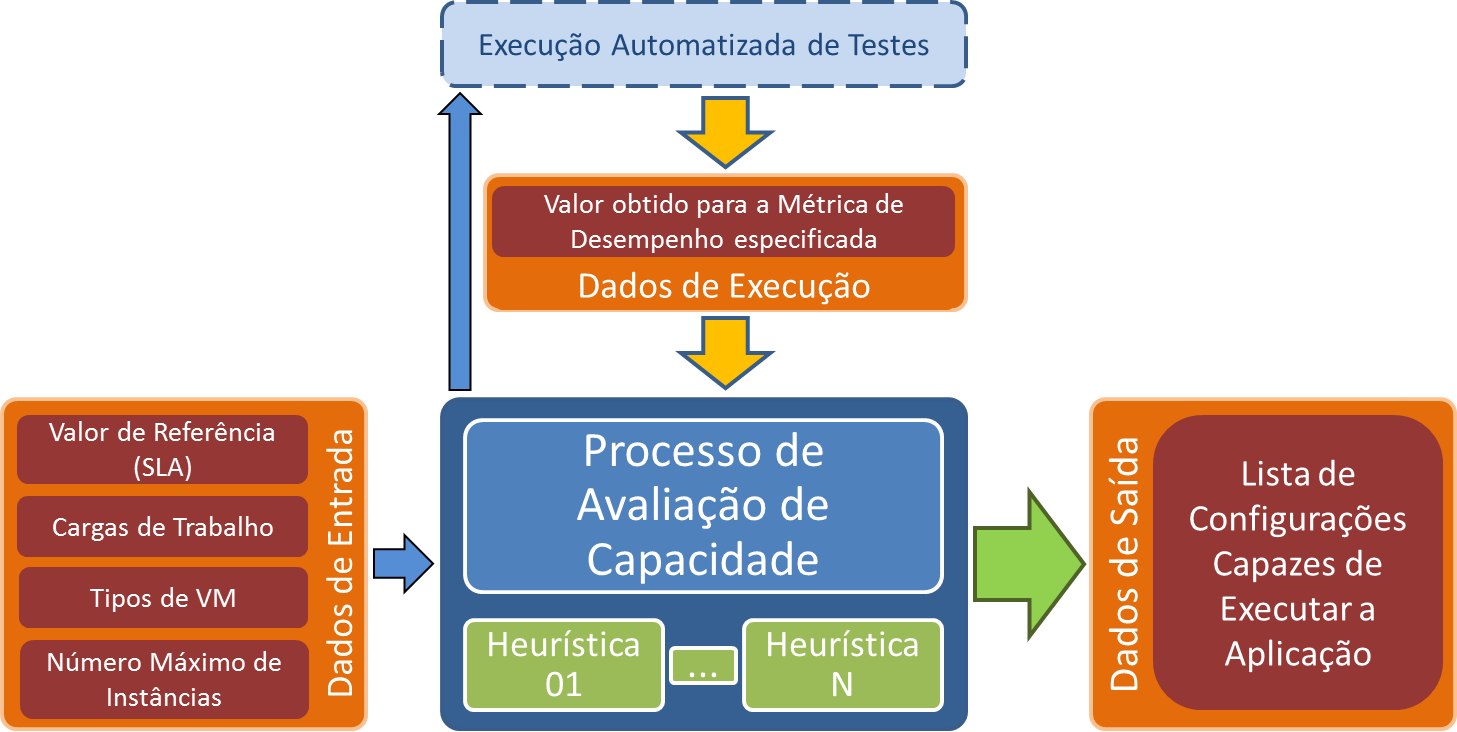
\includegraphics[scale=0.6]{img/processoAltoNivel}
  \end{center}
  \caption{\label{fig:fig_processo_alto_nivel}Visão geral do Processo de
  Avaliação de Capacidade.}
\end{figure}

Este capítulo aborda em detalhes todas as fases do processo 
proposto, explicando quais são os dados de entrada necessários, as operações 
executadas pelo processo e quais as decisões pelas quais o processo tem que 
passar até determinar quais são as Configurações de menor custo capazes de 
executar a Aplicação.

\subsection{Dados de Entrada}

O principal parâmetro esperado pelo processo de avaliação de capacidade é o Valor
de Referência de Desempenho, ou SLA. Esse valor será usado para determinar 
se a Aplicação atingiu os requisitos mínimos de desempenho exigidos, conforme
veremos na descrição do funcionamento do processo, mais adiante.

Além do SLA, o processo precisa também conhecer quais são as Cargas de Trabalho
para as quais o desempenho da Aplicação sob Teste deverá ser avaliado. Porém,
nem todas as Cargas de Trabalho serão impostas de fato à Aplicação. Isso vai 
depender do conjunto de decisões tomadas pelo processo com base na comparação do 
resultado obtido pela Aplicação com o SLA. Ainda assim, graças à sua característica 
de inferência de desempenho, o processo mostra resultados para todas as Cargas de 
Trabalhado informadas como parâmetro de entrada.

Para que o desempenho da Aplicação seja avaliado, é preciso que o processo conheça 
quais são as Configurações disponibilizadas no Provedor de nuvem para esse fim. 
Para isso, o processo deve ser alimentado com uma lista de Tipos de Máquinas Virtuais 
que serão utilizadas na execução da Aplicação, bem como a quantidade máxima de 
instâncias usadas para compor cada Configuração. Através desses dados o processo
passa a conhecer então o Espaço de Implantação disponível para os testes de 
desempenho, composto por uma lista de Configurações geradas a partir da lista de
Tipos de Máquinas Virtuais disponíveis e do número máximo de instâncias.

\subsection{Atividades Customizáveis}
O processo de avaliação de capacidade proposto é um processo extensível, do qual
fazem parte atividades customizáveis para as quais são delegadas funções de
cunho mais específico, como a comunicação com o Provedor de nuvem e a Aplicação sob Teste
para fins de orquestração do teste de desempenho, e também funções para as quais
é desejado um certo grau de flexibilidade a fim de tornar o processo mais adaptável,
como a escolha das Cargas de Trabalho e Configurações que serão usadas na execução
da Aplicação.

\subsubsection{Execução dos Testes de Desempenho}
Todas as atividades ligadas à rotina de execução da Aplicação, desde sua implantação,
passando pela criação e configuração das máquinas virtuais no ambiente do Provedor 
de nuvem, bem como pelo controle de inicialização e finalização dessas instâncias, 
serviços subjacentes como bancos de dados e filas, e a própria parametrização da 
execução e parada da Aplicação em si não fazem parte do escopo do processo. Este,
por sua vez, presume que os dados de resultado para cada execução estarão disponíveis
quando necessários. A maneira como esses dados serão de fato obtidos é
encapsulada pela implementação concreta desta atividade do processo.

%dependente da implementação concreta do processo e é irrelevante do ponto de
%vista do seu funcionamento.  

Portanto, o processo prevê a customização da atividade de Execução dos Testes,
que será responsável pelas ações necessárias à execução da Aplicação sob Teste no ambiente
alvo. A atividade customizada deverá conhecer os detalhes inerentes à comunicação com 
o Provedor e com a Aplicação sob Teste e, assim, ser capaz de ordenar a sua execução e 
coletar como resposta os dados de desempenho esperados pelo processo. Esse é um dos 
pontos de extensibilidade oferecidos pelo processo, cuja implementação concreta está 
fora do escopo deste trabalho. Vale destacar que o foco do processo proposto não está na automação de execução de testes de qualquer natureza, mas na análise dos dados resultantes dessa execução.

\subsubsection{Estratégias e Heurísticas}
\label{subsubsec:heuristicas}
De modo análogo à abordagem adotada em relação às atividades de execução dos
testes, as operações de seleção da Configuração sobre as quais a Aplicação
sob Teste será executada, bem como a seleção das Cargas de Trabalho a que ela 
será submetida durante sua execução, não são executadas diretamente pelo processo.
Nesse caso, são delegadas a uma atividade customizada que chamamos de Estratégia de 
Avaliação ou, simplesmente, Estratégia. Seu objetivo é permitir a aplicação de 
diferentes métodos para a escolha da melhor Configuração e/ou Carga de Trabalho 
mais adequada aos objetivos da avaliação de capacidade em curso e também ao perfil 
da Aplicação.

Como veremos na seção~\ref{sec:funcionamento_processo}, em diversas oportunidades
durante a execução do processo se faz necessária a seleção de uma Configuração de
maior ou menor capacidade. Do mesmo modo, em certos momentos o processo precisa
que uma Carga de Trabalho menor ou maior seja selecionada. A partir dessas escolhas
o processo é capaz de navegar no Espaço de Implantação submetendo a Aplicação sob
Teste a diferentes cenários de Cargas de Trabalho em diversas condições de capacidade
computacional.

Um problema relacionado à execução de testes de desempenho em ambientes de nuvem
é que o próprio teste implica num custo financeiro que pode ser bastante elevado
caso o Espaço de Implantação definido seja muito extenso. O mesmo se dá com 
relação à lista de Cargas de Trabalho. A fim de minimizar esse problema, este
trabalho propõe a técnica de inferência de desempenho explicada
detalhadamente na seção~\ref{subsec:processo_niveis_capacidade}, através da
qual será possível eliminar grande parte das execuções reais da Aplicação
durante os testes, reduzindo assim o custo total da avaliação.

Porém, outro problema enfrentado na busca pela melhor Configuração capaz de executar 
uma Aplicação está justamente no momento de selecionar, dentre um conjunto de 
Configurações possíveis, qual a mais promissora a ser usada para uma execução real, 
dado que não é conhecido previamente o potencial computacional dessas Configurações.

A fim de solucionar esse problema, este trabalho introduz o conceito das 
Heurísticas de Seleção, que são abordagens a serem observadas no momento em que
a Estratégia de Avaliação deve escolher a próxima Configuração ou a próxima Carga 
de Trabalho. 

Foi definido um conjunto de 3 abordagens aplicáveis ao Espaço de Implantação,
ou seja, à escolha da próxima Configuração a ser testada, e outras 3 abordagens
aplicáveis à lista de Cargas de Trabalho. A combinação dessas abordagens dá origem
a 9 Heurísticas de Seleção, a saber:

\begin{samepage}
\begin{description}
  \item[OO - Otimista/Otimista] \hfill \\ Visa selecionar Configurações menores e Cargas de Trabalho maiores
  \item[OC - Otimista/Conservadora] \hfill \\ Visa selecionar Configurações menores e Cargas de Trabalho intermediárias
  \item[OP - Otimista/Pessimista] \hfill \\ Visa selecionar Configurações e Cargas de Trabalho menores
  \item[CO - Conservadora/Otimista] \hfill \\ Visa selecionar Configurações intermediárias e Cargas de Trabalho maiores
  \item[CC - Conservadora/Conservadora] \hfill \\ Visa selecionar Configurações e Cargas de Trabalho intermediárias
  \item[CP - Conservadora/Pessimista] \hfill \\ Visa selecionar Configurações intermediárias e Cargas de Trabalho menores
  \item[PO - Pessimista/Otimista] \hfill \\ Visa selecionar Configurações e Cargas de Trabalho maiores
  \item[PC - Pessimista/Conservadora] \hfill \\ Visa selecionar Configurações maiores e Cargas de Trabalho intermediárias
  \item[PP - Pessimista/Pessimista] \hfill \\ Visa selecionar Configurações maiores e Cargas de Trabalho menores
\end{description}
\end{samepage}

Para um melhor entendimento de como as Heurísticas influenciam a navegação do 
processo entre as Configurações que compõem o Espaço de Implantação a ser explorado
e também entre as Cargas de Trabalho a serem impostas sobre a Aplicação, convém
observar a Figura~\ref{fig:heuristicas}.

\begin{figure}[t]
  \begin{center}
    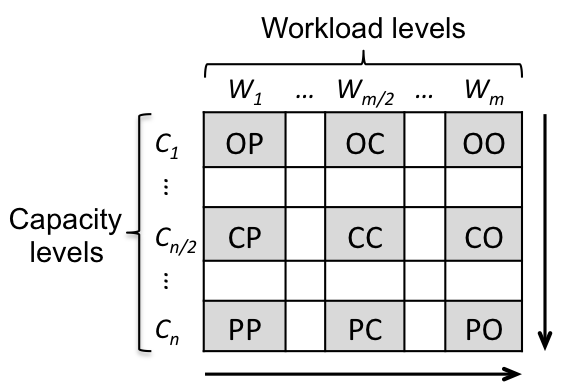
\includegraphics[scale=.8]{img/heuristics}
  \end{center}
  \caption{\label{fig:heuristicas}Ilustração das estratégias de seleção de Configurações e Cargas de Trabalho utilizadas pelas 9 Heurísticas de Seleção.}
\end{figure}

A imagem ilustra dois conjuntos dispostos em forma de matriz, um conjunto 
na vertical, formando as linhas, composto de $n$ Configurações $C_1 \ldots C_{n/2} 
\ldots C_n$ e um conjunto composto de $m$ Cargas de Trabalho $W_1 \ldots W_{m/2} 
\ldots W_m$, formando as colunas. As células dessa matriz mostram as Heurísticas
que selecionariam o par formado pela Configuração e pela Carga de Trabalho referentes
à linha e coluna da célula. Nessa representação das Heurísticas, a primeira letra
refere-se à abordagem usada para a escolha da Configuração e a segunda letra refere-se 
à abordagem usada na escolha da Carga de Trabalho.
 
Podemos ver, então, que as Heurísticas com abordagem Otimista escolherão Configurações 
mais próximas a $C_1$ e Cargas de Trabalho mais próximas a $W_m$. Por serem otimistas, essas 
abordagens consideram que máquinas menores são capazes de executar a aplicação com o nível esperado de desempenho sob cargas 
mais severas.

Ainda com base na mesma imagem, vemos que as abordagens conservadoras se concentram
nas células intermediárias, conforme a descrição das Heurísticas. A Heurística
OC, otimista para Configurações e conservadora para Cargas, se concentra na 
primeira linha, ou seja, mais próxima de $C_1$, e nas colunas do centro, mais
próximas de $W_{n/2}$. Observação similar se faz para a Heurística PO, pessimista 
para Configurações e otimista para Cargas, concentrando-se nas últimas linhas e 
últimas colunas, ou seja, Configurações e Cargas maiores.

Voltando a tratar das Estratégias de Avaliação, estas serão responsáveis por efetuar
a escolha de Configurações e Cargas de Trabalho implementando a lógica prevista pelas
Heurísticas. Enquanto as Heurísticas são lógicas que indicam as proximidades onde 
deve ser feita a escolha de Configurações e Cargas, a Estratégia implementa de fato
um algoritmo que reflita o comportamento esperado pela ideia da Heurística.
 
A aplicação das Heurísticas de Seleção, através da implementação de Estratégias 
de Avaliação, está intrinsecamente ligada aos objetivos deste trabalho, que é estudar 
os efeitos da inferência de desempenho na eficiência do processo de avaliação de 
capacidade para aplicações em ambientes de nuvem IaaS. A inteligência 
das Heurísticas propostas, ou seja, sua capacidade de escolher corretamente as 
Configurações e Cargas de Trabalho, é determinante para o sucesso do processo e 
da técnica de inferência. A eficácia e efetividade da aplicação das heurísticas
é analisada no Capítulo~\ref{chap:resultados}. 

\section{Funcionamento do Processo}
\label{sec:funcionamento_processo}
Para efeito de entendimento do funcionamento geral do processo de avaliação de 
capacidade ora proposto, podemos abstrair temporariamente o comportamento das 
Heurísticas. Esta é, aliás, outra vantagem da abordagem adotada de 
delegação de funções específicas a atividades customizadas: além da flexibilidade e 
adaptabilidade, a abstração dessas operações torna mais fácil o entendimento, 
a descrição e a implementação concreta do processo.

\begin{figure}
  \begin{center}
    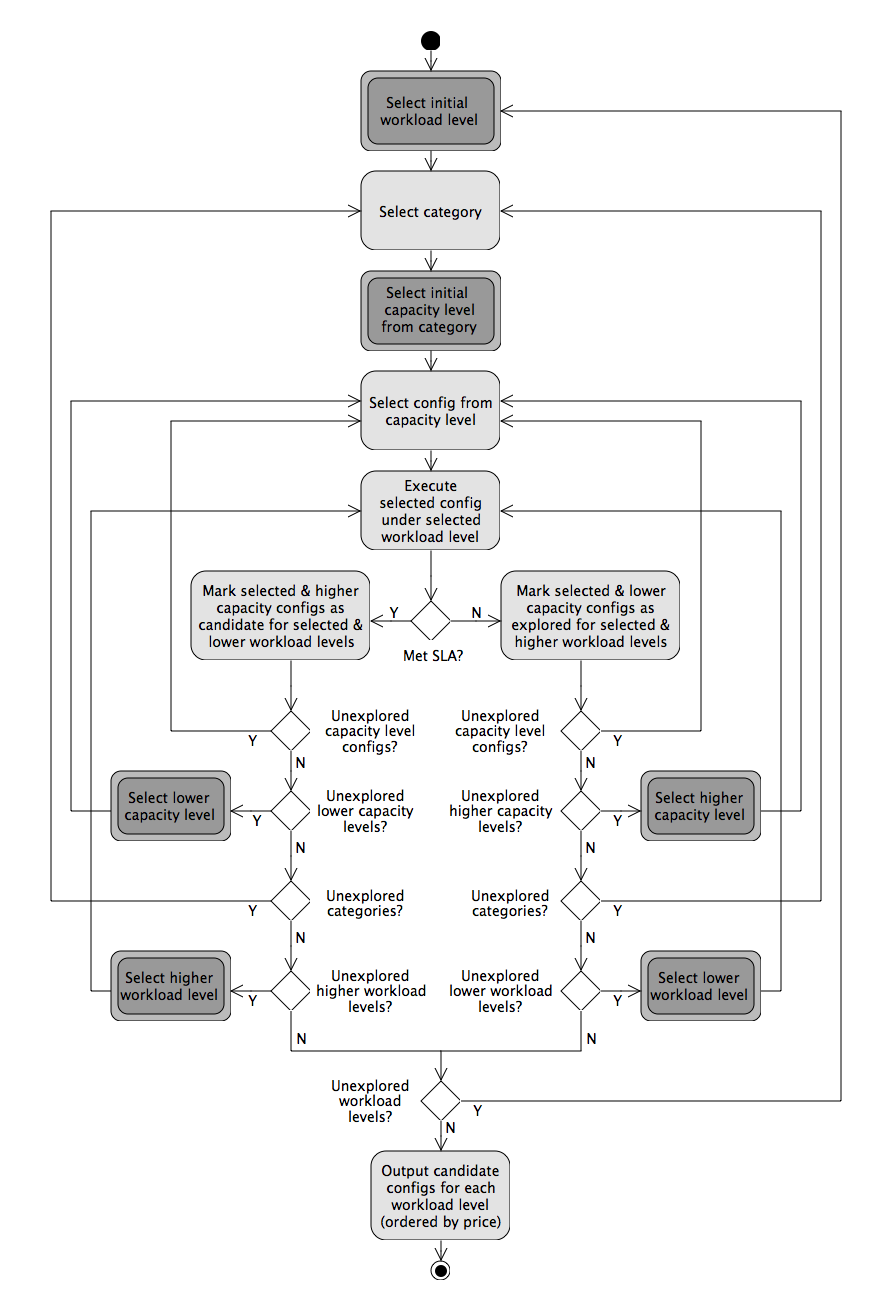
\includegraphics[scale=0.5]{img/capacity-planning-diagram-v13-mono}
  \end{center}
  \caption{\label{fig:fig_processo_aval_capacidade}Diagrama de atividades do Processo de Avaliação de Capacidade.}
\end{figure}


No diagrama de atividades representado na Figura~\ref{fig:fig_processo_aval_capacidade}, os blocos em destaque representam as operações que o processo espera que sejam executadas por uma Estratégia de 
Avaliação que implemente alguma das Heurísticas propostas na seção anterior. Os outros 
blocos referem-se a ações comuns do próprio processo, executadas de maneira 
idêntica independentemente de qual seja a Aplicação sob Teste ou de qual seja a 
Estratégia de Avaliação usada. A delegação de funções para a atividade de Execução
de Testes não está destacada no diagrama e se dá no passo ``\emph{Executar
config sob nível de carga}'', situado aproximadamente no centro da figura.

\subsection{Operações iniciais}
\label{subsec:processo_operacoes_iniciais}
Uma vez tendo recebido os dados de entrada, o Processo tem seu início com o momento 
de escolher por onde começar a execução dos testes.

A primeira atividade desempenhada pelo Processo é a escolha da Carga de Trabalho
inicial. A Estratégia é solicitada para realizar esta escolha, que deve
seguir a orientação dada pela lógica da Heurística selecionada para 
a avaliação. Assim, será escolhido
um volume de carga maior se a Heurística for Otimista, um volume menor se a
Heurística for Pessimista, ou um volume intermediário se a Heurística for Conservadora. 

Depois de selecionar o nível de carga, o processo segue para selecionar a
Categoria. Conforme as definições apresentadas na Seção~\ref{subsec:definicoes_categorias}, 
os Tipos de Máquinas Virtuais oferecidos pelo Provedor são normalmente agrupados 
por Categorias, que reunem máquinas de propósito e atributos semelhantes. Dessa
forma, o Espaço de Implantação sobre o qual a avaliação de capacidade se dará está 
dividido em Categorias. O número de Categorias envolvidas na avaliação depende do 
conjunto de Tipos de Máquinas Virtuais selecionados pelo usuário e passados como
parte dos dados de entrada do Processo.

O Processo de Avaliação seleciona a primeira
Categoria de máquinas a ser explorada. O processo não especifica a ordem ou método 
dessa escolha, pois essa ordem não é importante uma vez que todas as Categorias 
presentes no Espaço de Implantação serão avaliadas. Conforme veremos no 
Capítulo~\ref{chap:capacitor}, a implementação de referência do Processo 
desenvolvida neste trabalho escolhe a primeira Categoria em ordem alfabética pelo
nome. Outras implementações do processo podem optar por outros métodos de
escolha.



\subsubsection{Níveis de Capacidade}
\label{subsec:processo_niveis_capacidade}
Dando continuidade à sequência de operações iniciais dentro do Processo de Avaliação 
de Capacidade, o próximo passo prevê que a Estratégia de Avaliação deve selecionar 
um Nível de Capacidade inicial. 

Níveis de Capacidade são um conceito criado para ajudar a estabelecer uma hierarquia 
sobre as relações de capacidade de processamento entre as diversas Configurações. 
Essa hierarquia de capacidade é válida apenas entre Configurações de uma mesma 
Categoria de Máquinas Virtuais. 

Para cada Categoria, o Nível ``um'' de Capacidade é composto apenas pela Configuração 
de menor preço dentro da Categoria. Um novo nível é criado com todas as Configurações 
para as quais é verdadeira a relação ``maior que''. Considera-se que uma 
Configuração $C_1$ é ``maior que'' uma outra Configuração $C_2$ se: 

\begin{enumerate}[label=\bfseries \alph*)]
\item ambas são formadas pelo mesmo Tipo de Máquina Virtual e $C_1$ possui 
número maior de instâncias do que $C_2$; ou
\item ambas são formadas pelo mesmo número de instâncias
e o Tipo de Máquina de $C_1$ possui mais CPU e mais memória que o Tipo de Máquina
de $C_2$.  
\end{enumerate}

Esse, então, passa a ser o Nível 
``dois'' e a lógica se repete daí em diante, tomando-se, para cada Configuração 
desse nível, as imediatamente maiores, formando um novo Nível. O procedimento 
continua até que todas as Configurações estejam devidamente classificadas em 
Níveis de Capacidade.

A Figura~\ref{fig_niveis_capacidade} mostra um pequeno exemplo, onde 6 Configurações,
pertencentes a duas Categorias distintas, foram classificadas em dois Níveis de 
Capacidade dentro de cada Categoria. Os retângulos representam as Configurações, 
com o texto indicando o nome do Tipo de Máquina Virtual utilizado e o número entre 
parênteses representando a quantidade de instâncias que compõem a Configuração. 
As setas que ligam as Configurações indicam a existência da relação de capacidade 
entre elas apontando da menor para a maior. A ausência de seta entre duas Configurações 
implica a impossibilidade de se afirmar uma relação de capacidade entre elas. 

\begin{figure}[t]
  \begin{center}
    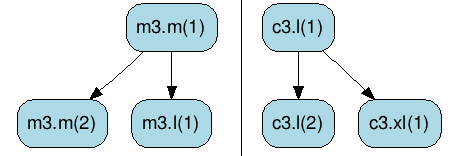
\includegraphics[scale=.65]{img/exemplo-niveis-capacidade}
  \end{center}
  \caption{\label{fig_niveis_capacidade}Agrupamento de Configurações por Níveis de Capacidade}
\end{figure}

Assim, observando o Espaço de Implantação organizado por Categorias e classificado
hierarquicamente, a Estratégia deve selecionar, com base em uma das Heurísticas 
propostas na subseção anterior, um Nível de Capacidade inicial. As 
Configurações que fazem parte do Nível inicial escolhido são disponibilizadas 
para que a Avaliação proceda com a execução dos testes da Aplicação.

\subsection{Execução do Teste de Desempenho}
\label{subsec:processo_execucao}
Após a escolha da Carga de Trabalho inicial e do primeiro Nível de Capacidade a
ser avaliado, uma Configuração deve ser tomada a partir do Nível de Capacidade 
atual. Essa seleção não segue nenhuma regra específica, uma vez que todas as 
Configurações do Nível de Capacidade devem ser avaliados, ainda que por meio da técnica de 
Inferência de Desempenho, vista adiante.
 
Executa-se, então, a Aplicação sob Teste, impondo-se a ela a Carga de Trabalho 
selecionada, e analisa-se o resultado dessa execução. Nesse ponto o Processo se 
bifurca, atingindo seu primeiro ponto de decisão.

Esse é o momento em que a técnica de Inferência, conforme propomos neste trabalho,
será aplicada. A análise do Resultado obtido, mais especificamente do valor atribuído
à Métrica de Desempenho avaliada, comparado ao parâmetro do Valor de Referência (SLA), 
determina se a Aplicação é ou não capaz de atender à demanda imposta pela
Carga de Trabalho. Vejamos a seguir uma explanação mais detalhada a respeito das
inferências que sucedem essa análise.  

\subsection{Inferência de Desempenho}
O processo de Inferência de Desempenho acontece logo após a análise comparativa
do Resultado, conseguinte a uma execução real da Aplicação sob Teste em uma 
Configuração, que foi tomada a partir de um Nível de Capacidade previamente 
selecionado. Durante essa execução, foi imposta sobre a Aplicação uma Carga de 
Trabalho, também previamente selecionada.

Observando o diagrama da Figura~\ref{fig:fig_processo_aval_capacidade}, podemos 
ver, bem ao centro, o ponto de decisão que define o sucesso ou o fracasso da 
Aplicação em atingir o SLA exigido. 

Se o desempenho da Aplicação satisfaz o SLA proposto, o Processo considera que a
Configuração é capaz de executar sob a Carga de Trabalho imposta e diz que a 
Configuração atual (sobre a qual a Aplicação acabou de ser executada) deve ser
assinalada como uma Configuração Candidata.

Neste ponto, a técnica de Inferência de Desempenho é aplicada e, como vemos
no texto do diagrama do Processo, todas as Configurações maiores que a atual também
são assinaladas como Candidatas. Ora, se identificamos que uma certa Configuração
consegue executar a Aplicação sob uma certa Carga de Trabalho, é intuitivo o 
pensamento de que qualquer Configuração que possua maior poder computacional 
também seja capaz de executar a mesma Aplicação sob a mesma Carga de Trabalho.

Assim, usando a representação do Espaço de Implantação conforme descrito na
Seção~\ref{subsec:processo_niveis_capacidade}, o Processo assinala como candidatas
todas as Configurações para as quais, direta ou indiretamente, a Configuração 
atual aponte, ou seja, todas as Configurações que, de acordo com o grafo de capacidade representado no Espaço de Implantação, seriam ``maiores que'' a Configuração atual. 

Mas a técnica de Inferência ainda vai mais longe. Sabendo que as Configurações
que acabaram de ser assinaladas como Candidatas são capazes de executar a Aplicação
sob a Carga de Trabalho atual, também é intuitivo concluir que Cargas de Trabalho 
menores, ou mais brandas, serão naturalmente atendidas por essas mesmas Configurações.

Então, com base na Inferência de Desempenho, o Processo marca
a Configuração atual e todas as maiores que ela como Candidatas não só para a 
Carga de Trabalho atual, mas também para todas as Cargas inferiores à atual.

De volta ao ponto de decisão da análise do Resultado em relação ao SLA, caso o 
desempenho da Aplicação não satisfaça o SLA, o Processo considera que a 
Configuração não é capaz de executar sob a Carga de Trabalho atual. Assim, essa
Configuração é marcada como Rejeitada para tal Carga.

De forma coerente, a lógica de Inferência de Desempenho entende que, se dada 
Configuração não consegue executar uma Aplicação a contento sob uma certa Carga,
intuitivamente, as Configurações menores tampouco conseguirão. Assim, o processo
indica a marcação de todas as Configurações ``menores que'' a atual como 
Rejeitadas para a Carga de Trabalho atual. 

Ainda seguindo a Inferência de Desempenho, quando uma Configuração não consegue
atender a demanda de uma Carga de Trabalho, presume-se que também não consiga
atender a demandas maiores, ou mais severas. O Processo de Avaliação marca, então,
a Configuração atual e todas as Configurações menores que ela como Rejeitadas para todas as Cargas de Trabalho maiores que a Carga atual. 

\begin{figure}[t]
  \begin{center}
    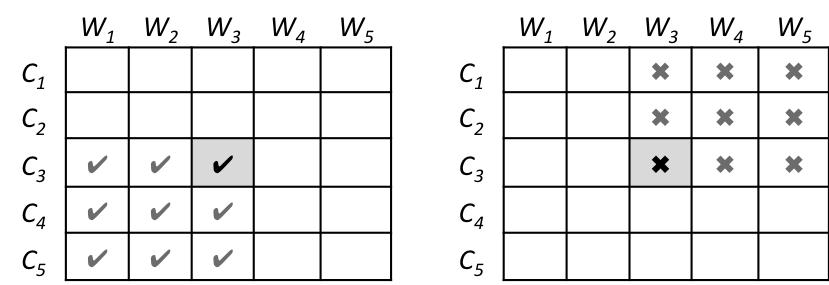
\includegraphics[scale=.8]{img/inference}
  \end{center}
  \caption{\label{fig:fig_processo_inferencia}Ilustração da marcação de Configurações Candidatas (à esquerda) e Rejeitadas (à direita) com a técnica de Inferência de Desempenho.}
\end{figure}

O efeito da utilização da técnica de Inferência de Desempenho pode ser melhor
visualizado através dos exemplos mostrados na Figura~\ref{fig:fig_processo_inferencia}. A figura mostra 
duas situações: a da esquerda para o caso em que o SLA é satisfeito e a da direita 
caso o SLA não seja satisfeito. Em ambos os casos vemos uma célula central realçada, 
indicando que a Aplicação sob Teste foi executada na Configuração $C_3$ sob a 
Carga de Trabalho $W_3$. As células assinaladas com com um ``\boldmath$\surd{}$'' mostram as Configurações
marcadas como Candidatas para as Cargas de Trabalho correspondentes. As células
assinaladas com um ``\boldmath$\times{}$'' representam as Configurações marcadas como Rejeitadas.

Essa representação serve para demonstrar a contribuição da utilização da técnica 
de Inferência na execução de testes de desempenho. Nesse exemplo, foram 
explorados 9 cenários diferentes, dados pelas combinações de Configurações e 
Cargas de Trabalho, mas apenas 1 execução real foi conduzida. Isso significa não
só que o tempo total gasto na Avaliação de Capacidade é reduzido, mas também o
custo financeiro envolvido nessa atividade. 

Mais adiante neste capítulo, expandiremos essa representação para mostrar a ação
da Inferência de Desempenho após várias iterações do laço compreendido pelo 
Processo de Avaliação. Por hora, continuemos com a descrição dos passos seguintes.

\subsection{Seleção dos Próximos Cenários}
\label{subsec:selecao_cenarios}
Passada a fase de Inferência de Desempenho, o processo segue seu caminho, tomando
as decisões que levarão à seleção dos cenários seguintes a serem avaliados quanto
à sua capacidade.

O ponto de decisão que sucede a marcação das Configurações Candidatas ou Rejeitadas
checa se existem Configurações pertencentes ao atual Nível de Capacidade cujas 
execuções ainda não tenham sido avaliadas para a Carga de Trabalho atual. Se 
existirem, o Processo volta ao passo de seleção de uma Configuração a partir do 
Nível de Capacidade e uma nova execução é solicitada.

Se não existirem Configurações inexploradas para a Carga de Trabalho atual no
Nível de Capacidade corrente, o Processo buscará por um Nível de Capacidade que 
ainda não tenha sido completamente explorado. Se a Aplicação satisfez o SLA na 
execução anterior, a Estratégia deverá selecionar um Nível de Capacidade menor. 
Se o SLA não tiver sido atingido, a Estratégia tentará selecionar um  Nível de 
Capacidade maior. Depois de selecionado o próximo Nível de Capacidade, o laço do
Processo retorna ao ponto de seleção da próxima Configuração e outra execução 
acontece.
   
Novo ponto de decisão surge quando a Estratégia não encontra um Nível de 
Capacidade a ser explorado. Nessa situação, o Processo procura uma outra
Categoria dentro do Espaço de Implantação que ainda possua pelo menos uma
Configuração ainda não explorada para a Carga de Trabalho atual. Se houver,
o Processo retorna ao passo de seleção de um Nível de Capacidade dentro da
Categoria selecionada e nova execução será realizada.

Caso não haja uma outra Categoria com Configurações não avaliadas, atingimos
então um outro ponto de decisão, onde a Estratégia deve buscar uma Carga 
de Trabalho que não tenha sido avaliada. Se a execução anterior atingiu o SLA,
uma Carga de Trabalho maior será buscada. Caso contrário, a Estratégia tentará
uma Carga menor que a atualmente selecionada. Se a Estratégia obtiver sucesso
nessa escolha, o Processo dispara uma nova execução da Aplicação com a Configuração
corrente e sob a Carga de Trabalho que acabou de ser selecionada.

Porém, se a Estratégia não conseguir fornecer uma Carga de Trabalho segundo as 
restrições do Processo definidas a partir da comparação do Resultado com o SLA, o Processo 
voltará ao passo inicial de seleção de Carga de Trabalho, que não tem qualquer 
restrição quanto a essa seleção. Tentará assim a escolha de uma Carga inexplorada
qualquer. Caso não seja encontrada nenhuma Carga de Trabalho inexplorada, significa
que não há mais nada a ser testado e o Processo é encerrado.

\subsection{Finalização da Avaliação}
Não tendo mais Configurações a serem testadas sob nenhuma Carga de Trabalho, o 
Processo é dado por concluído e sua finalização se efetiva pela apresentação de uma
lista que contém, para cada Carga de Trabalho, as Configurações capazes de executar
a Aplicação sob Teste, em ordem crescente de preço.

Por ``capazes de executar'', entenda-se como as Configurações para as quais o valor
obtido para a Métrica de Desempenho durante a execução da Aplicação sob determinada
Carga de Trabalho é menor ou igual ao valor definido para o SLA
como parte dos dados de entrada do Processo.

Embora essa seja a resposta final do processo, a contribuição real deste trabalho está
na maneira como chegamos a essa resposta, com redução de custo e tempo, e na precisão 
da resposta, ou seja, o nível de acerto atingido pelo Processo ao apontar as Configurações
Candidatas e Rejeitadas. Dados reais que comprovam a eficácia do 
Processo e da técnica de Inferência de Desempenho propostos são apresentados no
Capítulo~\ref{chap:resultados}, que trata dos experimentos realizados e analisa criticamente os resultados obtidos.

Para deixar mais clara essa contribuição, a seguir é dado um exemplo que ilustra os vários momentos
em que a técnica de Inferência de Desempenho é empregada durante a execução do Processo, e que evidencia a influência que a utilização de diferentes Heurísticas de Seleção exerce sobre a sua eficiência em selecionar as melhores configurações de recursos para a aplicação alvo.

\section{Exemplo de Utilização do Processo}

\begin{figure}
  \begin{center}
    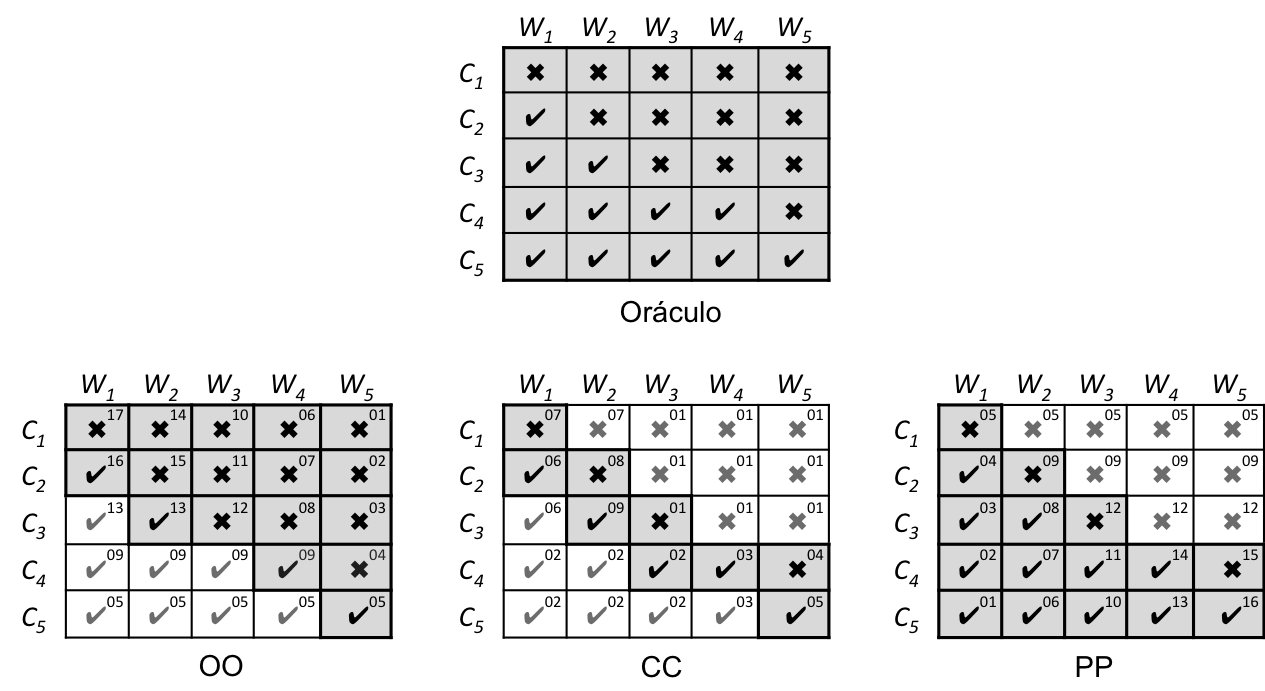
\includegraphics[scale=0.7]{img/rastros}
  \end{center}
  \caption{\label{fig:fig_processo_traces}Ilustração da Inferência de Desempenho com Diferentes Heurísticas de Seleção.}
\end{figure}

A Figura~\ref{fig:fig_processo_traces} mostra, nos quadros da parte inferior, 
o rastro de todas as iterações da execução do Processo de Avaliação com 3 
Heurísticas de Seleção distintas: Otimista/Otimista, Conservadora/Conservadora e 
Pessimista/Pessimista. O quadro da parte superior da imagem mostra o que seria o
resultado da execução real da aplicação em todos os cenários analisados, ou seja,
com todas as combinações de Configurações e Cargas de Trabalho. A essa 
representação damos o nome de Oráculo, por conter toda a informação real de
desempenho da Aplicação sob Teste considerada em cada cenário.

O Oráculo serve-nos de base de referência para a apuração da eficácia do Processo
e sua Inferência de Desempenho, ou seja, a precisão de acerto quanto a quais são
de fato as Configurações capazes de executar a Aplicação com desempenho que atenda
ao SLA. Além disso, com base no Oráculo, podemos também aferir qual a eficiência 
da Heurística utilizada na Avaliação, medindo a economia em número de execuções
reais e, por conseguinte, em tempo e custo financeiro da Avaliação.

As execuções reais são representadas nas figuras pelas células destacadas, mais 
escuras. Novamente, as células marcadas com um ``\boldmath$\surd{}$'' indicam que a Aplicação atingiu um
desempenho que cumpre o SLA exigido para aquela combinação de Configuração e Carga
de Trabalho, ou seja, a Configuração é considerada Candidata para aquela Carga. As
células marcadas com um ``\boldmath$\times$'' mostram onde a Aplicação não conseguiu cumprir 
o SLA, ou seja, as Configurações Rejeitadas.

Dentro de cada célula nos quadros que mostram o comportamento das Heurísticas há
um número que indica em qual passo da iteração do processo a Configuração foi
marcada como Candidata ou Rejeitada. Alguns números são repetidos em várias células
e isso serve para mostrar a Inferência de Desempenho atuando. As células brancas
foram marcadas como Candidatas ou Rejeitadas por meio da técnica de Inferência no
passo denotado pelo pequeno número no canto da célula. Note-se que para as células 
destacadas os números não se repetem e demonstram a ordem de escolha das Configurações
pela Heurística para execução real da Aplicação.

O exemplo apresentado na Figura~\ref{fig:fig_processo_traces} mostra uma eficácia
de 100\%, ou seja, usando a Inferência de Desempenho, o Processo indicou com correção todas as
Configurações que, caso fossem testadas de fato, com uma execução real da Aplicação,
teriam um desempenho dentro do SLA esperado. A figura mostra, ainda, que, para a 
Aplicação fictícia considerada, a Heurística Conservadora/Conservadora foi a mais
eficiente, com apenas 9 execuções reais contra um potencial total de 25 execuções.
Supondo que o tempo de execução dos testes de desempenho da Aplicação é o mesmo 
em cada iteração, isso representa uma economia de 64\% no tempo de execução da
Avaliação de Capacidade em comparação com a execução de todos os cenários.

Outra contribuição trazida pelo emprego das Heurísticas de Seleção de
Configurações é a automação da decisão de por onde começar a execução dos testes. Quando se faz
necessária a análise do comportamento de uma aplicação qualquer em um determinado
ambiente, com dezenas ou até centenas de variações tanto do ambiente como dos 
volumes de demanda, a escolha de uma combinação inicial dessas variáveis é um
problema de difícil solução.

O emprego das Heurísticas de Seleção ajuda não só na escolha da Configuração e 
da Carga de Trabalho iniciais, mas também de qual a próxima combinação a ser 
testada e sempre visando ao menor custo de execução dessa avaliação.

O Capítulo~\ref{chap:resultados} irá mostrar os resultados obtidos
com o Processo de Avaliação proposto neste trabalho ao avaliar uma
Aplicação real em um ambiente também real de nuvem IaaS. Serão apresentados
resultados de eficiência e eficácia do emprego da técnica de Inferência de Desempenho
e das Heurísticas de Seleção, comparando-as sob diversos SLAs.

\section{Resumo}
Este capítulo apresentou uma proposta de processo de avaliação de capacidade
cuja ideia chave é a inferência de capacidade de uma configuração de recursos a partir dos dados 
reais de desempenho obtidos por uma outra configuração de recursos semelhante, mas de capacidade
presumidamente menor ou maior.

Essa proposta de processo se apoia na hipótese de que é possível estabelecer uma
relação de capacidade entre os recursos disponibilizados por um provedor de nuvem
IaaS. Com base nessa hipótese, definiu-se uma sequência de passos
que visam a identificar quais recursos são capazes de executar uma determinada 
aplicação sob determinados volumes de carga de trabalho com o menor número
possível de execuções reais da aplicação. Como resultado, o processo busca
a redução de custo e tempo normalmente envolvidos na atividade de avaliação de
capacidade dos recursos disponíveis na nuvem.

O Capítulo~\ref{chap:capacitor}, a seguir, apresentará uma visão mais concreta,
com a descrição do arcabouço de software desenvolvido neste trabalho como implementação de referência
para o processo proposto. Além disso, será apresentada uma aplicação web desenvolvida para
ilustrar o uso do processo de avaliação de capacidade
baseado em inferência de desempenho. 

%Essa aplicação foi usada para demonstração da criação de algumas Estratégias
% criadas e para a execução dos testes de eficácia e efetividade das técnicas propostas, bem como das próprias
%Estratégias, e cujos resultados apresentaremos no
% Capítulo~\ref{chap:resultados} mais adiante.
   
% ----------------------------------------------------------

% ----------------------------------------------------------

% ----------------------------------------------------------
% Cloud Capacitor
% ----------------------------------------------------------
\chapter{Implementação do Processo}
\label{chap:capacitor}
% ----------------------------------------------------------
A fim de confirmar as hipóteses de eficácia e eficiência do emprego do Processo
de Avaliação de Capacidade descrito no capítulo anterior, bem como da técnica de
Inferência de Desempenho e das Heurísticas de Seleção que dão suporte a esse Processo, 
criamos uma implementação concreta de sua especificação na forma de uma biblioteca
extensível e de um sistema computacional que demonstra seu funcionamento fazendo
a avaliação de uma aplicação real em um provedor de nuvem de infraestrutura.

Demos o nome de CloudCapacitor à biblioteca, implementada como uma \emph{gem} da
linguagem Ruby~\cite{ruby}. Desenvolvemos o sistema computacional Capacitor Web 
para ser uma interface visual para a utilização do CloudCapacitor, usando 
o \emph{framework} Ruby on Rails~\cite{rails}.  

Descrevemos a seguir os detalhes da implementação de cada um e como ambos se
relacionam para oferecer ao usuário a experiência da avaliação de capacidade
de baixo custo e alta precisão prevista pelo Processo proposto, com uma interface
amigável e de fácil utilização.

\section{CloudCapacitor}
CloudCapacitor é uma biblioteca para criação de sistemas de avaliação de 
capacidade em ambientes de nuvem de infraestrutura como serviço. É a implementação
completa da especificação do Processo de Avaliação de Capacidade do 
Capítulo~\ref{chap:processo}, permitindo que sejam customizadas as atividades 
definidas pelo Processo como pontos de extensão, como as Estratégias de Avaliação
e o disparo e controle da execução da Aplicação sob Teste.

Vamos iniciar a apresentação do CloudCapacitor pelas classes que compõem a biblioteca
e suas responsabilidades. Em seguida, veremos como CloudCapacitor auxilia 
desenvolvedores de software na criação de sistemas de avaliação de capacidade,
mostrando o fluxo de utilização da biblioteca através de sua interface de programação.
Depois, falaremos sobre alguns detalhes de implementação da biblioteca, como 
a solução para representação do Espaço de Implantação e seu papel na execução do
Processo de Avaliação de Capacidade. Por fim, apresentaremos os pontos de extensão
da biblioteca, notadamente como implementar um Executor, a classe responsável pelo
controle de execução da Aplicação sob Teste, e como sobrescrever a Estratégia de
Avaliação fornecida pela biblioteca a fim de alterar seu comportamento padrão.

Para concluir a apresentação do CloudCapacitor, será mostrada a saída de dados
fornecida pela biblioteca com as Configurações capazes de executar a
Aplicação sob Teste em cada uma das Cargas de Trabalho respeitando o SLA definido.

\subsection{Classes e Responsabilidades}
\label{subsec:classes}
CloudCapacitor é formado por um conjunto de classes que, juntas representam os
componentes envolvidos na avaliação de capacidade de aplicações em ambientes de
nuvem, de acordo com os conceitos e o Processo definidos anteriormente, nos
Capítulos~\ref{chap:formalizacao} e~\ref{chap:processo}. A Figura~\ref{fig:classes}
mostra as principais classes cujas responsabilidades e cooperação levam ao 
resultado final de uma Avaliação. 

Ao utilizar a biblioteca CloudCapacitor na construção de um software para avaliação
de capacidade, o desenvolvedor tem à sua disposição uma classe principal, chamada
\emph{Cacitor}. Essa classe fornece o fluxo principal do Processo de Avaliação, com todos
os seus pontos de decisão e de extensão.

\begin{figure}[htb]
  \caption{\label{fig:classes}Principais classes que compõem o CloudCapacitor e suas relações}
  \begin{center}
    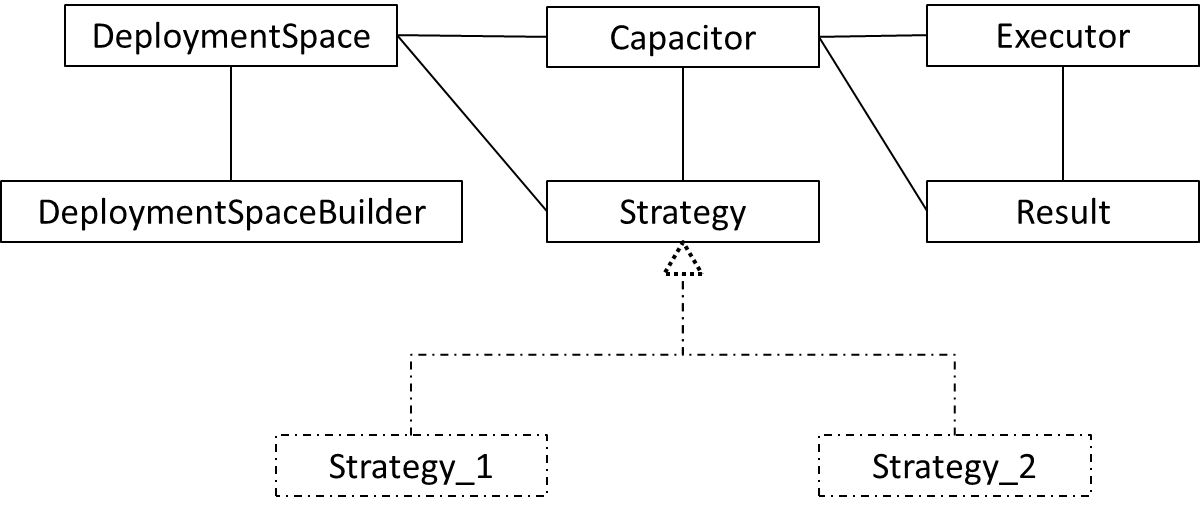
\includegraphics[scale=0.75]{img/CapacitorClasses}
  \end{center}
\end{figure}

Entre os pontos de extensão, destacamos o uso da classe \emph{Strategy}. Como 
vemos na Figura~\ref{fig:classes}, essa classe é fornecida pela biblioteca e a
notação de linhas pontilhadas denota a sua possibilidade de especialização, onde,
sobrescrevendo alguns de seus métodos, é possível criar Estratégias com comportamento
diversificado.

A classe \emph{DefaultExecutor} é o outro ponto de extensão oferecido pela biblioteca.
Porém, neste caso, o desenvolvedor deve mandatoriamente implementar uma subclasse
que forneça a lógica necessária ao controle da execução do teste de desempenho.
Na figura, a classe a ser implementada pelo desenvolvedor é representada com o 
nome de \emph{RealExecutor}.

Para que a Avaliação de Capacidade possa ser efetuada, a classe \emph{Capacitor}
deve conhecer o resultado de cada execução da Aplicação sob Teste, de modo que
possa tomar as decisões corretas na indicação das Configurações Candidatas e
Rejeitadas. Esses resultados são encapsulados na classe \emph{Result}, cujos 
objetos são fornecidos pela subclasse responsável pela execução dos testes de 
desempenho.

E, finalmente, durante a execução da Avaliação de Capacidade, a classe \emph{Capacitor} 
precisa ter conhecimento do Espaço de Implantação disponibilizado. Essa é a 
responsabilidade da classe \emph{DeploymentSpace}, que implementa uma estrutura 
de dados em memória para representar os diversos Níveis de Capacidade formados 
entre as Configurações. A construção dessa estrutura é responsabilidade da classe 
\emph{DeploymentSpaceBuilder}, que contém os algoritmos necessários à preparação 
do grafo usado para navegação pelos Níveis de Capacidade. 

\subsection{Fluxo de Utilização da Biblioteca}
\label{subsec:fluxo}
CloudCapacitor foi criada para ser uma ferramenta de auxílio na construção de 
aplicações destinadas à condução de testes para avaliação de capacidade,
visando basicamente a reusabilidade e a simplicidade na composição dessas 
aplicações.

Embora tenha sido desenvolvida objetivando sua utilização na construção de 
aplicações web baseadas no framework Ruby on Rails, CloudCapacitor pode facilmente
ser usada em todo tipo de aplicação escrita em Ruby, desde scripts puros até
aplicações baseadas em outros frameworks.

Em suma, o fluxo de utilização da biblioteca é bastante simples e pode ser 
descrito por:

\begin{enumerate}
  \item Configurar parâmetros de criação do Espaço de Implantação 
  \item Identificar Tipos de Máquinas Virtuais para o Espaço de Implantação
  \item Instanciar um objeto \emph{Capacitor}
  \item Atribuir ao \emph{Capacitor} um objeto \emph{DefaultExecutor}
  \item Atribuir ao \emph{Capacitor} um objeto \emph{Strategy}
  \item Executar o método \emph{run\_for} do \emph{Capacitor}
\end{enumerate}

Antes que a aplicação que está sendo desenvolvida possa de fato dar início ao uso 
da biblioteca, é preciso que o desenvolvedor a configure previamente. 

O primeiro passo é configurar os limites de tamanho do Espaço de Implantação e 
isso deve ser feito através de um arquivo em formato YAML~\cite{yml}. A localização 
e o nome do arquivo de parâmetros para a criação do Espaço de Implantação dependem 
de como a aplicação está sendo implementada: se for uma aplicação Ruby on Rails, 
deverá haver um arquivo chamado \emph{capacitor.yml} na pasta \emph{config}, que 
fica dentro da pasta raiz da aplicação; caso contrário, deverá haver um arquivo 
chamado \emph{capacitor\_settings.yml} já na pasta raiz da aplicação ou na mesma 
pasta em que está o script que invoca a biblioteca. 

A Figura~\ref{fig:settings} mostra um exemplo de conteúdo do arquivo que configura
os limites do Espaço de Implantação. São apenas dois parâmetros:

\begin{description}
  \item[max\_price] \hfill \\ O custo máximo que uma Configuração pode atingir
  \item[max\_num\_instances] \hfill \\ Número máximo de instâncias usadas em uma Configuração 
\end{description}

\begin{figure}[h]
  \caption{\label{fig:settings}Parâmetros de Configuração para o CloudCapacitor}
 \begin{lstlisting}[linewidth=\textwidth,xleftmargin=.04\textwidth, numbers=left]
deployment_space:
  #The maximum price for a whole Configuration.
  #This refers to the individual VM_Type price multiplied 
  #by the number of instances that make up the Configuration
  max_price: 7.0

  #The maximum number of instances in a Configuration. 
  #This is for horizontal scaling.
  max_num_instances: 4
  \end{lstlisting}
\end{figure}

No exemplo acima, serão criadas Configurações com 1, 2, 3 e 4 instâncias para cada
Tipo de Máquina Virtual especificada, desde que o custo total da Configuração não
ultrapasse o valor de 7,00 unidades monetárias.

O próximo passo na utilização do CloudCapacitor é especificar quais serão os Tipos
de Máquinas Virtuais utilizados na geração do Espaço de Implantação. Essa 
especificação é feita em outro arquivo em formato YAML, discriminando as 
características de CPU, Memória e custo de cada Tipo de Máquina para que o
CloudCapacitor possa gerar os Níveis de Capacidade usados para inferência de
desempenho. O caminho onde esse arquivo deve ser entrado precisa ser passado 
como parâmetro na inicialização do objeto Capacitor. Caso não seja informado, o 
CloudCapacitor procurará um arquivo pelo nome \emph{deployment\_space.yml}, na
pasta \emph{config}, se for uma aplicação Ruby on Rails, ou na pasta raiz do
script ou outro tipo de aplicação.
 
\begin{figure}[h]
  \caption{\label{fig:depspace}Especificação de Tipos de Máquinas para o Espaço de Implantação}
 \begin{lstlisting}[linewidth=\textwidth,xleftmargin=.04\textwidth, numbers=left]
---
- !ruby/object:CloudCapacitor::VMType
  name: m2.xlarge
  cpu: 6.5
  mem: 17.1
  price: 0.41
  category: m2
- !ruby/object:CloudCapacitor::VMType
  name: c1.xlarge
  cpu: 20
  mem: 7.0
  price: 0.58
  category: c1
- !ruby/object:CloudCapacitor::VMType
  name: m1.xlarge
  cpu: 8
  mem: 15.0
  price: 0.48
  category: m1
- !ruby/object:CloudCapacitor::VMType
  name: m2.4xlarge
  cpu: 26
  mem: 68.4
  price: 1.64
  category: m2
  \end{lstlisting}
\end{figure}

A Figura~\ref{fig:depspace} mostra a especificação de um conjunto de Tipos de
Máquinas Virtuais oferecidos pelo serviço EC2 do Provedor Amazon Web 
Services~\cite{ec2}. São disponibilizadas para o CloudCapacitor máquinas 
\emph{m2.xlarge}, \emph{c1.xlarge}, \emph{m1.xlarge} e \emph{m2.4xlarge} e, para
cada uma, podemos ver as características de CPU, memória RAM e preço, conforme
informados pelo Provedor. Esses são os dados que serão usados na criação do Espaço
de Implantação, atendendo às restrições de tamanho e custo impostas no passo 
anterior, de forma que os testes sejam executados conforme o proposto
no Processo de Avaliação de Capacidade.

Feitas as configurações necessárias, o desenvolvedor pode, assim, criar um objeto 
a partir da classe \emph{Capacitor} e, então atribuir a ele um objeto instanciado
a partir de uma subclasse de \emph{DefaultExecutor}, subclasse esta de sua própria
implementação e que forneça os meios necessários para administração da execução
dos testes de desempenho da Aplicação sob Teste.

\begin{figure}[h]
  \caption{\label{fig:mincode}Código Ruby para execução do CloudCapacitor}
 \begin{lstlisting}[language=Ruby,linewidth=\textwidth,xleftmargin=.04\textwidth, numbers=left]
    capacitor = Capacitor.new
    capacitor.executor = Executors::DummyExecutor.new
    capacitor.strategy = Strategies::Strategy.new

    capacitor.strategy.approach workload: :optimistic,
                                config:   :conservative

    candidates = capacitor.run_for [100,200,300,400,500]
    
    total_cost = capacitor.run_cost
    total_executions = capacitor.executions  
 \end{lstlisting}
\end{figure}

Observamos na Figura~\ref{fig:mincode} os passos de instanciação do Capacitor,
na linha 1. Na linha seguinte, um objeto da classe \emph{DummyExecutor}, que é
apenas didática, já é atribuído ao \emph{Capacitor}.

A partir da linha 3, começamos a ver os passos seguintes da utilização do 
CloudCapacitor, com a definição de uma Estratégia de Avaliação, configurada
com uma Heurística de Seleção do tipo OC (v. Seção~\ref{sec:heuristicas}).
A execução da Avaliação de Capacidade acontece de fato na chamada que ocorre
na linha 8, onde são passados valores que representam uma lista de grandezas de
Cargas de Trabalho que serão impostas à Aplicação sob Teste rodando sobre as
Configurações geradas a partir do Espaço de Implantação.

Ao final da Avaliação, o Capacitor retorna a lista de Configurações Candidatas
para cada valor de Carga de Trabalho passado como parâmetro. Adicionalmente, o
desenvolvedor tem à sua disposição alguns dados a respeito da própria Avaliação,
como o número total de execuções da Aplicação sob Teste no ambiente de nuvem e o  
custo total acarretado por essas execuções. 

Agora que já temos uma visão geral dos componente e da utilização do CloudCapacitor,
passemos a uma descrição um pouco mais detalhada do que acontece durante a atividade
de Avaliação de Capacidade.

\subsection{Funcionamento Interno}
\label{subsec:capacitor_funcionamento}
Uma vez demonstrado o modelo de utilização da biblioteca e explicadas as relações
entre as diversas classes que a compõem, podemos detalhar alguns aspectos da
implementação que ajudarão a esclarecer melhor como todas essas partes agem em
conjunto para executar, da forma como proposto no Capítulo~\ref{chap:processo},
o Processo de Avaliação de Capacidade.

Nesta seção mostraremos inicialmente as linhas gerais da implementação da classe 
responsável pelo controle da execução dos testes de desempenho. Mostraremos em 
seguida como a biblioteca representa o Espaço de Implantação de forma que os 
Níveis de Capacidade sejam usados para navegar entre Configurações e como a 
Inferência de Desempenho atua sobre esses dados. Explicamos ainda como pode ser 
feita a customização de uma Estratégia de Avaliação a fim de alterar o 
comportamento de uma Heurística. Será também apresentado um exemplo de saída do 
resultado apresentado pela classe Capacitor ao final da execução de uma Avaliação.

\subsubsection{Controle da Execução}
\label{subsubsec:funcionamento_executor}
O controle da execução da Aplicação sob Teste no ambiente de nuvem é feito por 
meio de um objeto instanciado de uma classe que deve ser criada pelo
desenvolvedor que está utilizando o CloudCapacitor na implementação de sua 
ferramenta de Avaliação de Capacidade.

Para que tudo funcione a contento, a classe criada deve ser extendida a partir
da classe \emph{DefaultExecutor} fornecida pelo CloudCapacitor. A única 
exigência feita para essa subclasse é que ela implemente um método:

\begin{itemize}
  \item Com a assinatura \emph{run(configuration, workload)}; e
  \item Que retorne um objeto da classe \emph{Result}
\end{itemize}

Ou seja, a classe criada pelo desenvolvedor deve pelo menos apresentar um método
\emph{run} que receba como parâmetros uma Configuração e um valor para a Carga 
de Trabalho que será imposta sobre a Aplicação. O retorno desse método deve ser
um objeto da classe \emph{Result}, que deve ser inicializado com apenas 3 atributos:

\begin{description}
  \item[\emph{value}] \hfill \\
    O valor obtido pela Aplicação para a Métrica de Desempenho estudada
  \item[\emph{cpu}] \hfill \\
    O percentual de CPU consumido pela Aplicação durante o teste
  \item[\emph{mem}] \hfill \\
    O percentual de Memória RAM utilizada pela Aplicação durante o teste
\end{description}

Essas informações devem ser obtidas pelo desenvolvedor através de chamadas a
uma ferramenta de execução de testes, como \cite{cunha2012ambiente}, 
\cite{jayasinghe2012} ou \cite{silva2013cloudbench}. A implementação dessa 
comunicação com a ferramenta de automação de testes escolhida é efetuada está 
fora do escopo deste trabalho e deve ficar a cargo do desenvolvedor prover o 
código que controle a execução dos testes e obtenha os valores de desempenho
e consumo de CPU e memória.

O método \emph{run}, implementado na subclasse criada a partir de 
\emph{DefaultExecutor}, é chamado pelo objeto \emph{Capacitor} nos momentos em
que novas execuções são necessárias, conforme descrito na 
Seção~\ref{subsec:processo_execucao}. O objeto \emph{Result} retornado é usado
na comparação com o SLA especificado pelo usuário do sistema como Valor de
Referência para indicar se a Aplicação atendeu ou não ao requisito de desempenho.

De posse dessa resposta, o \emph{Capacitor} tem condições de prosseguir no seu
processamento, marcando as Configurações como Candidatas ou Rejeitadas e 
escolhendo as próximas Configurações a serem executadas. Essas ações se baseiam
no caminhamento sobre o Espaço de Implantação, cuja implementação passamos a
descrever a seguir.

\subsubsection{Espaço de Implantação}
\label{subsubsec:funcionamento_depspace}
O uso do CloudCapacitor começa com as configurações de como a 
biblioteca vai montar o Espaço de Implantação, apontando-se quais as restrições 
e quais os Tipos de Máquinas disponíveis para realização dos testes.

No momento em que o desenvolvedor instancia um objeto da classe \emph{Capacitor},
uma das primeiras tarefas da biblioteca é exatamente proceder à montagem de uma
estrutura que represente o Espaço de Implantação de forma que as Heurísticas
possam navegar entre as Configurações e que a rotina que implementa o Processo de
Avaliação possa identificar, por meio da técnica de Inferência de Desempenho, 
quais são as Configurações Candidatas e Rejeitadas. 

\begin{figure}[htb]
  \caption{\label{fig:depspace_real}Representação interna de um Espaço de Implantação no CloudCapacitor}
  \begin{center}
    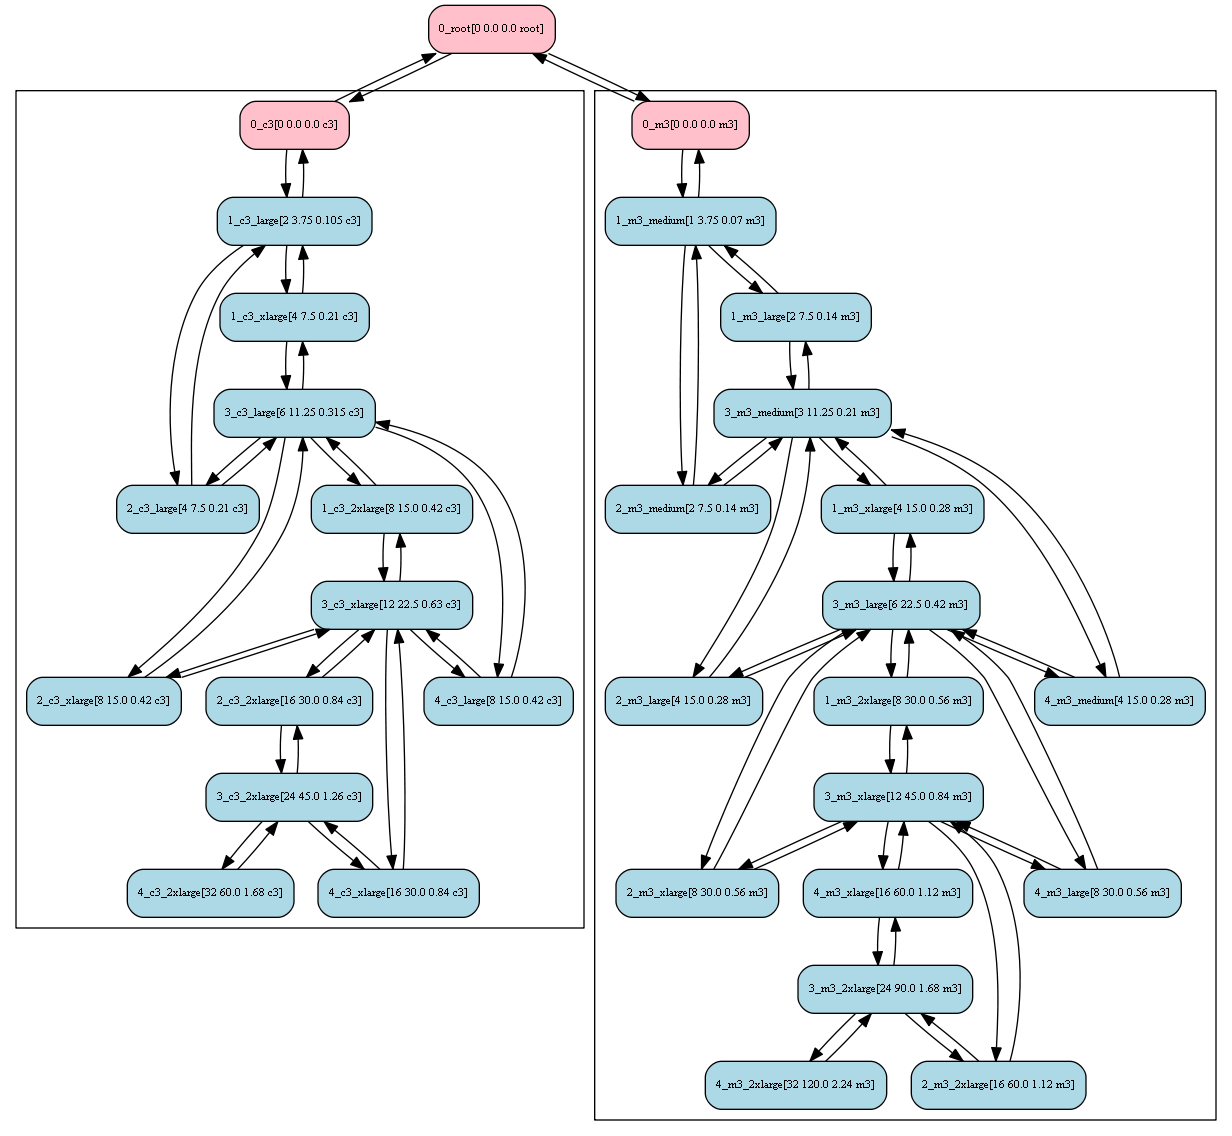
\includegraphics[scale=0.35]{img/exemplo_grafo_espaco_implantacao}
  \end{center}
\end{figure}

Como é possível ver na Figura~\ref{fig:depspace_real}, o Espaço de Implantação é 
representado internamente por um grafo bi-direcionado onde os nós são as 
Configurações. Arestas existem entre nós onde sejam verdadeiras as relações 
``maior que'' e ``menor que'', conforme as definições da 
Seção~\ref{sec:formalizacao_configuracoes}. O grafo precisa ser bi-direcionado 
para permitir que a navegação a partir de uma determinada Configuração seja feita 
tanto para as Configurações ``maiores'' quanto para as ``menores''.

CloudCapacitor separa o Espaço de Implantação em subgrafos, agrupando as
Configurações por Categoria de Máquinas Virtuais. Cada subgrafo é destinado às
Configurações cujo Tipo de Máquina pertença a uma determinada Categoria. O primeiro
nó, observado no topo do grafo, é o nó raiz e serve apenas para estabelecer a 
separação e permitir o trânsito entre as Categorias.

As classes \emph{DeploymentSpace} e \emph{DeploymentSpaceBuilder} implementam
a geração do Espaço de Implantação com base na relação de capacidade ou na relação
de preço entre as Configurações. O desenvolvedor pode optar pelo grafo por capacidade ou por preço no momento da
instanciação do objeto \emph{Capacitor}. Embora esse não seja o foco desta 
pesquisa, isso foi feito para que pudesse ser estudada a influência da formação 
do Espaço de Implantação na precisão e eficiência de custo das Heurísticas de 
Seleção. Discutiremos a respeito desses resultados no Capítulo~\ref{chap:resultados} 
adiante.

O Espaço de Implantação é a estrutura que dá suporte à navegação das Estratégias
sobre os diversos Níveis de Capacidade no momento em que devem ser escolhidas
as próximas Configurações a serem testadas. Suporta também a técnica de Inferência 
de Desempenho na identificação das relações de tamanho e/ou preço entre as 
Configurações nos pontos onde o Processo marca as Candidatas ou Rejeitadas, 
mostrando-se como um ponto chave para o sucesso do Processo de Avaliação.

Descreveremos a seguir a implementação e o funcionamento das Estratégias de 
Avaliação e como o desenvolvedor pode criar sua própria Estratégia que melhor
supra suas necessidades de seleção de Configurações. 

\subsubsection{Estratégias de Avaliação}
\label{subsubsec:funcionamento_estrategias}
A Estratégia de Avaliação é responsável por aplicar uma Heurística de 
Seleção de Configurações nos momentos em que o Processo precisa navegar
pelo Espaço de Implantação. Assim, a cada momento em que um novo Nível 
de Capacidade deve ser escolhido, segundo o fluxo de ações previsto no 
Processo de Avaliação proposto, a Estratégia é invocada e age conforme 
a implementação da Heurística selecionada para a Avaliação.

CloudCapacitor fornece uma classe chamada \emph{Strategy} como uma implementação
padrão para as 9 Heurísticas descritas no Capítulo~\ref{chap:processo}. A
Figuras~\ref{fig:strategy_workload_code}~e~\ref{fig:strategy_capacity_code}
mostram o código fonte dos métodos de seleção de Carga de Trabalho e Nível
de Capacidade, respectivamente.

\begin{figure}[h]
  \caption{\label{fig:strategy_workload_code}Seleção de Carga de Trabalho na classe \emph{Strategy}}
  \begin{lstlisting}[language=Ruby,linewidth=\textwidth,xleftmargin=.04\textwidth, numbers=left]
  def select_workload( workload_list )
    case @wkl_approach
      when :pessimistic
        workload_list.first
      when :optimistic
        workload_list.last
      when :conservative
        workload_list[ workload_list.size / 2 ]
    end
  end
  \end{lstlisting}
\end{figure}

\begin{figure}[h]
  \caption{\label{fig:strategy_capacity_code}Seleção de Nível de Capacidade na classe \emph{Strategy}}
  \begin{lstlisting}[language=Ruby,linewidth=\textwidth,xleftmargin=.04\textwidth, numbers=left]
  def take_a_capacity_level_from( unexplored_levels )
    levels = unexplored_levels.keys
    return [] if levels.empty?
    case @cfg_approach
      when :pessimistic
        unexplored_levels.assoc( levels[-1] )
      when :optimistic
        unexplored_levels.assoc( levels[0] )
      when :conservative
        unexplored_levels.assoc( levels[levels.size / 2] )
    end
  end
  \end{lstlisting}
\end{figure}

Porém,
é possível substituir essa classe por uma mais adequada aos objetivos do
usuário.

A interface da classe \emph{Capacitor} permite que 

Figura~\ref{fig:mincode}

***RASCUNHO***
CloudCapacitor
OK  Diagrama de Classes (UML) / Arquitetura de Componentes
OK  Enumeração das classes e suas responsabilidades
OK  Fluxo de utilização da biblioteca (caixa preta, interface com o Capacitor)
OK  Especificação e Carregamento do Deployment Space
  Executor - Implementação
  Estratégia - Descrição da interface
  Estratégia - Como sobrescrever (Gof Strategy Pattern)
  Apresentação do resultado da avaliacao
Capacitor Web
  Apresentação da interface de entrada
  Resultados
  Trace
  Full Trace
Resumo e transicao para o proximo capitulo
***RASCUNHO***



PorémAo instanciar um objeto da classe Capacitor, o desenvolvedor deve atribuir  
Por padrão, o CloudCapacitor oferece uma Estratégia de Avaliação que implementa 
uma lógica simples para as Heurísticas de Seleção de Configurações definidas no
capítulo anterior. Essa lógica pode ser facilmente sobrescrita conforme a necessidade
do usuário ou o perfil da Aplicação sob Teste.


****RASCUNHO
\subsection{Heuristicas}
Para que uma Heurística de Avaliação de Capacidade seja compatível no âmbito deste trabalho, 
deve apresentar um conjunto mínimo de operações esperadas para que a lógica da
avaliação se complete e o resultado final obtido possa ser considerado válido e
comparável com os resultados obtidos por outras Heurísticas.

Além disso, as operações constituem a interface pela qual o controlador das 
sessões de avaliação pode configurar as Heurísticas e informar-lhe os dados 
necessários ao controle da sua execução.
 
Apresentamos esse conjunto mínimo de operações nas subseções a seguir, que 
representam o arcabouço necessário para a construção de uma Heurística de 
Avaliação de Capacidade.
 
% ----------------------------------------------------------

% ----------------------------------------------------------

% ----------------------------------------------------------
% Resultados
% ----------------------------------------------------------
\chapter{Experimentos e Resultados}
\label{chap:resultados}
% ----------------------------------------------------------
Este capítulo vem apresentar os experimentos realizados como forma de
verificação do Processo de Avaliação de Capacidade por Inferência de 
Desempenho proposto no Capítulo~\ref{chap:processo}. Inicialmente é
apresentada a metodologia utilizada para construção dos experimentos, 
com a descrição da Aplicação sob Teste escolhida, como foi implantada e 
como foram realizadas as execuções para coleta de dados de desempenho. Depois
são apresentados os resultados obtidos por cada uma das 9 Heurísticas ao
fazer a Avaliação de Capacidade da Aplicação. Esses resultados são usados 
para uma comparação qualitativa das Heusrísticas entre si e para atestar
a eficiência do Processo de Avaliação de Capacidade proposto e sua técnica 
de Inferência de Desempenho tanto quanto à economia de tempo e custo como  
quanto à precisão de acerto de seuas predições.

\section{Metodologia}
\label{sec:resultados_metodologia}
A fim de validar a eficiência da Inferência de Desempenho no apoio
ao Planejamento de Capacidade, foram realizadas seções de avaliação de
capacidade de uma aplicação implantada em um provedor de nuvem de
infraestrutura como serviço.

A aplicação escolhida foi o WordPress \cite{wordpress}, um motor de construção 
e administração de \emph{blogs}. Sua escolha foi motivada por ser uma aplicação
bem conhecida, de utilização via web, ideal para implantação em ambiente de
nuvem, e com componentes arquiteturais escaláveis. Além disso, o fluxo de 
utilização típico apresenta características bem diversificadas quanto ao uso
de recursos de CPU e memória, rede, sistema de arquivos e banco de dados.

\begin{figure}[hbt]
  \begin{center}
    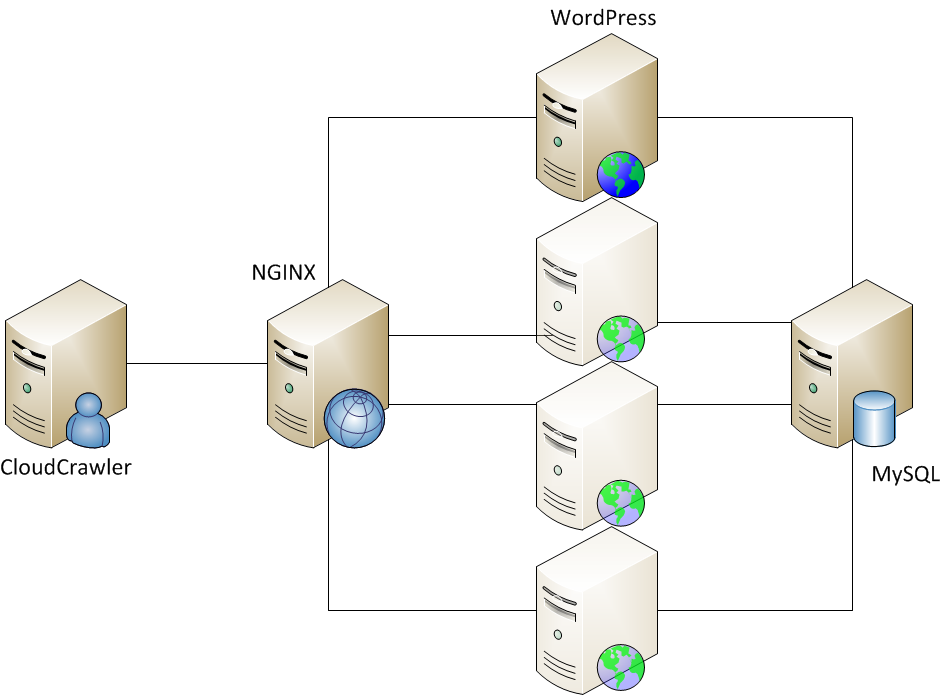
\includegraphics[scale=0.4]{img/ImplantacaoWordPress}
  \end{center}
  \caption{\label{fig:implantacao}Implantação do WordPress na AWS EC2 para Avaliação de Capacidade}
\end{figure}

O Provedor escolhido foi a Amazon, com seu serviço de infraestrutura AWS EC2
\cite{ec2}, onde o WordPress foi implantado em duas camadas: uma para o banco de 
dados MySQL, e outra para a aplicação, executada pelo servidor Apache HTTPD. Como
balanceador de carga, foi utilizada uma máquina executando o servidor web Nginx. A
Figura~\ref{fig:implantacao} mostra um panorama geral dessa implantação. 

Devido a restrições de custo e tempo, os experimentos foram limitados de forma a variar 
apenas a camada de aplicação, usando de 1 a 4 servidores Apache executando o WordPress. 
Na imagem, essa variação está representada pela suavização de cor das máquinas dessa 
camada, no sentido de que podem não estar presentes em certos cenários.

A execução dos testes foi orquestrada pelo Cloud~Crawler~\cite{cunha2012ambiente},
que automatizou as tarefas de iniciar e parar as todas as instâncias, configurar 
o balanceador de carga de acordo com o número de instâncias testadas na camada de 
aplicação, iniciar e parar a execução dos testes, controlando as Cargas de Trabalho
impostas à Aplicação sob Teste (o WordPress) e coletando os dados de desempenho 
para cada execução. 

De forma a viabilizar uma \emph{baseline} para validação e verificação das 
predições de desempenho inferidas pelo Processo de Avaliação implementado pela 
biblioteca CloudCapacitor, foram efetivamente executados testes de desempenho 
para todas as combinações de Configurações e Cargas de Trabalho. A esse conjunto
de dados reais de execução foi dado o nome de ``oráculo'' e esse procedimento
de teste de todas as possibilidades foi considerado como uma Heurística de ``Força
Bruta''. As 9 Heurísticas propostas no Capítulo~\ref{chap:processo} foram comparadas
entre si e com a Heurística de Força Bruta, que não faz qualquer inferência de
desempenho. O resultado dessas comparações serão analisados nas seções seguintes.

Para compor o Espaço de Implantação do experimento desenvolvido para este trabalho, 
foram escolhidos 7 Tipos de Máquinas Virtuais oferecidos pelo serviço EC2:

\begin{itemize}
  \item m3\_medium 
  \item m3\_large
  \item m3\_xlarge
  \item m3\_2xlarge
  \item c3\_large
  \item c3\_xlarge
  \item c3\_2xlarge
\end{itemize}

Para cada um desses Tipos de Máquinas, foram criadas Configurações com 1, 2, 3 e 4
instâncias, levando a um total de 28 Configurações diferentes no Espaço de Implantação,
divididas em duas Categorias distintas, ``C3'' e ``M3''. As Cargas de Trabalho
para este experimento foram quantificadas em número de usuários fazendo
requisições ao WordPress. Foram criadas 10 Cargas de Trabalho representando
100, 200, 300, 400, 500, 600, 700, 800, 900 e 1000 usuários. Com isso, foram
coletados dados de desempenho para 280 cenários diferentes, ou seja, foram 
testadas as 28 Configurações em cada uma das 10 Cargas de Trabalho especificadas 
para a Avaliação de Capacidade do WordPress na nuvem.

O teste de desempenho consistiu em fazer com que a Aplicação sob Teste WordPress
atendesse à demanda imposta pelo acesso de tantos usuários quanto especificados 
na Carga de Trabalho no período de 1 hora. Cada usuário disparava a seguinte
sequência de requisições:

\begin{enumerate}
  \item Efetuar \emph{logon}
  \item Inserir uma postagem
  \item Visitar uma postagem específica
  \item Alterar uma postagem
  \item Efetuar pesquisa por palavra-chave
  \item Alterar uma postagem
  \item Efetuar \emph{logoff}
\end{enumerate}

A Métrica de Desempenho usada no experimento foi ``Tempo de Resposta Total'', ou 
seja, o tempo total decorrido entre o envio da primeira requisição da sequência 
acima e o momento em que o cliente recebeu a resposta para última requisição da
sequência. Assim, para ser considerada como Candidata, uma Configuração devia 
ser capaz de atender 90\% dos conjuntos de requisições em um tempo total abaixo 
do tempo informado na entrada do parâmetro SLA.

A seguir serão discutidos os resultados obtidos com o Processo de Inferência de 
Desempenho e suas Heurísticas na indicação das Configurações capazes de executar
a Aplicação sob Teste sob vários níveis de demanda. Foram avaliadas a precisão do 
Processo na predição de capacidade e a economia de tempo e custo na execução
dos testes.

\section{Avaliação dos Resultados}
\label{sec:resultados_avaliacao}
A partir da execução do Processo de Inferência de Desempenho implementado pela
biblioteca CloudCapacitor, usada no desenvolvimento do Capacitor Web, foram 
realizadas Avaliações de Capacidade em 280 cenários de implantação do WordPress 
no serviço AWS EC2.

Com base nos resultados desses testes, foram avaliados os seguintes aspectos em
relação ao desempenho do Processo: 

\begin{description}
  \item[Acurácia] \hfill \\ Relação entre acertos e erros na predição de 
  capacidade das Configurações    
  \item[Eficiência] \hfill \\ Grau de redução do número de execuções reais e,
  consequentemente, do custo e do tempo total gasto nos testes de desempenho.
\end{description}

\subsection{Acurácia}
\label{subsec:resultados_precisao}
A avaliação da Acurácia das predições realizadas pelo Processo de Inferência visa 
a ratificar a expectativa de que, uma vez identificada uma relação de capacidade 
entre diferentes Configurações oferecidas por um Provedor de infraestrutura na 
nuvem, é possível inferir o desempenho de uma Aplicação executando em uma 
Configuração com base no desempenho observado em uma execução real da Aplicação 
em uma Configuração distinta.

\begin{table}[htbp]
  \centering
    {\fontsize{2.4mm}{1em}\selectfont
    \begin{tabular}{|c|c|c|c|c|c|c|c|c|c|c|c|c|c|c|c|}
    \hline
    \multirow{3}{*}{Heurísticas} & \multicolumn{15}{c|}{SLA (segundos)} \\
    \cline{2-16}
          & \multicolumn{3}{c|}{10} & \multicolumn{3}{c|}{20} & \multicolumn{3}{c|}{30} & \multicolumn{3}{c|}{40} & \multicolumn{3}{c|}{50} \\
          \cline{2-16}
          & P     & R     & F     & P     & R     & F     & P     & R     & F     & P     & R     & F     & P     & R     & F \\
          \hline          
    CC    & 1,00  & 1,00  & 1,00  & 1,00  & 1,00  & 1,00  & 1,00  & \textbf{\color{red}0,98}  & \textbf{\color{red}0,99}  & 1,00  & 1,00  & 1,00  & 1,00  & 1,00  & 1,00 \\
    CO    & 1,00  & 1,00  & 1,00  & 1,00  & 1,00  & 1,00  & \textbf{\color{red}0,99}  & 1,00  & \textbf{\color{red}0,99}  & 1,00  & 1,00  & 1,00  & 1,00  & 1,00  & 1,00 \\
    CP    & 1,00  & 1,00  & 1,00  & 1,00  & 1,00  & 1,00  & 1,00  & \textbf{\color{red}0,98}  & \textbf{\color{red}0,99}  & 1,00  & 1,00  & 1,00  & 1,00  & 1,00  & 1,00 \\
    OC    & 1,00  & 1,00  & 1,00  & 1,00  & 1,00  & 1,00  & \textbf{\color{red}0,99}  & \textbf{\color{red}0,99}  & \textbf{\color{red}0,99}  & 1,00  & 1,00  & 1,00  & 1,00  & 1,00  & 1,00 \\
    OO    & 1,00  & 1,00  & 1,00  & 1,00  & 1,00  & 1,00  & \textbf{\color{red}0,99}  & 1,00  & \textbf{\color{red}0,99}  & 1,00  & 1,00  & 1,00  & 1,00  & 1,00  & 1,00 \\
    OP    & 1,00  & 1,00  & 1,00  & 1,00  & 1,00  & 1,00  & 1,00  & \textbf{\color{red}0,98}  & \textbf{\color{red}0,99}  & 1,00  & 1,00  & 1,00  & 1,00  & 1,00  & 1,00 \\
    PC    & 1,00  & 1,00  & 1,00  & 1,00  & 1,00  & 1,00  & 1,00  & \textbf{\color{red}0,98}  & \textbf{\color{red}0,99}  & 1,00  & 1,00  & 1,00  & 1,00  & 1,00  & 1,00 \\
    PO    & 1,00  & 1,00  & 1,00  & 1,00  & 1,00  & 1,00  & \textbf{\color{red}0,99}  & 1,00  & \textbf{\color{red}0,99}  & 1,00  & 1,00  & 1,00  & 1,00  & 1,00  & 1,00 \\
    PP    & 1,00  & 1,00  & 1,00  & 1,00  & 1,00  & 1,00  & 1,00  & \textbf{\color{red}0,98}  & \textbf{\color{red}0,99}  & 1,00  & 1,00  & 1,00  & 1,00  & 1,00  & 1,00 \\
    \hline
    \end{tabular}%
    }% end fontsize
  \caption{\label{table:acuracia_capacidade}Acurácia da Inferência de Desempenho no Grafo por Capacidade}
\end{table}%

\begin{table}[htbp]
  \centering
  {\fontsize{2.4mm}{1em}\selectfont
    \begin{tabular}{|c|c|c|c|c|c|c|c|c|c|c|c|c|c|c|c|}
    \hline          
    \multirow{3}{*}{Heurísticas} & \multicolumn{15}{c|}{SLA (segundos)} \\
    \cline{2-16}
          & \multicolumn{3}{c|}{10} & \multicolumn{3}{c|}{20} & \multicolumn{3}{c|}{30} & \multicolumn{3}{c|}{40} & \multicolumn{3}{c|}{50} \\
          \cline{2-16}
          & P     & R     & F     & P     & R     & F     & P     & R     & F     & P     & R     & F     & P     & R     & F \\
          \hline
    CC    & 1,00  & 1,00  & 1,00  & 1,00  & 1,00  & 1,00  & 1,00  & \textbf{\color{red}0,97}  & \textbf{\color{red}0,98}  & 1,00  & 1,00  & 1,00  & 1,00  & 1,00  & 1,00 \\
    CO    & 1,00  & 1,00  & 1,00  & 1,00  & 1,00  & 1,00  & \textbf{\color{red}0,98}  & 1,00  & \textbf{\color{red}0,99}  & 1,00  & 1,00  & 1,00  & 1,00  & 1,00  & 1,00 \\
    CP    & 1,00  & 1,00  & 1,00  & 1,00  & 1,00  & 1,00  & 1,00  & \textbf{\color{red}0,97}  & \textbf{\color{red}0,98}  & 1,00  & 1,00  & 1,00  & 1,00  & 1,00  & 1,00 \\
    OC    & 1,00  & 1,00  & 1,00  & 1,00  & 1,00  & 1,00  & 1,00  & \textbf{\color{red}0,97}  & \textbf{\color{red}0,98}  & 1,00  & 1,00  & 1,00  & 1,00  & 1,00  & 1,00 \\
    OO    & 1,00  & 1,00  & 1,00  & 1,00  & 1,00  & 1,00  & \textbf{\color{red}0,98}  & 1,00  & \textbf{\color{red}0,99}  & 1,00  & 1,00  & 1,00  & 1,00  & 1,00  & 1,00 \\
    OP    & 1,00  & 1,00  & 1,00  & 1,00  & 1,00  & 1,00  & 1,00  & \textbf{\color{red}0,97}  & \textbf{\color{red}0,98}  & 1,00  & 1,00  & 1,00  & 1,00  & 1,00  & 1,00 \\
    PC    & 1,00  & 1,00  & 1,00  & 1,00  & 1,00  & 1,00  & \textbf{\color{red}0,99}  & \textbf{\color{red}0,97}  & \textbf{\color{red}0,98}  & 1,00  & 1,00  & 1,00  & 1,00  & 1,00  & 1,00 \\
    PO    & 1,00  & 1,00  & 1,00  & 1,00  & 1,00  & 1,00  & \textbf{\color{red}0,98}  & 1,00  & \textbf{\color{red}0,99}  & 1,00  & 1,00  & 1,00  & 1,00  & 1,00  & 1,00 \\
    PP    & 1,00  & 1,00  & 1,00  & 1,00  & 1,00  & 1,00  & \textbf{\color{red}0,99}  & \textbf{\color{red}0,97}  & \textbf{\color{red}0,98}  & 1,00  & 1,00  & 1,00  & 1,00  & 1,00  & 1,00 \\
    \hline
    \end{tabular}%
    }% end fontsize
  \caption{\label{table:acuracia_preco}Acurácia da Inferência de Desempenho no Grafo por Preço}
\end{table}%

Assim, este trabalho submeteu o Processo à verificação de sua acurácia ao realizar
predições para o desempenho do WordPress executando em máquinas virtuais do provedor
Amazon Web Services. O cálculo de Precision and Recall~\cite{powers2011evaluation} 
sobre os resultados dos experimentos realizados mostra que o Processo de Inferência 
de Desempenho é capaz de obter índices de precisão muito próximos de 100\%, como 
pode ser observado nas Tabelas~\ref{table:acuracia_capacidade}~e~\ref{table:acuracia_preco}. 

A Tabela~\ref{table:acuracia_capacidade} apresenta os dados de acurácia das 
predições realizadas usando-se o Espaço de Implantação estruturado pelas relações
de capacidade entre as Configurações. Já a Tabela~\ref{table:acuracia_preco} mostra
a acurácia das predições feitas utilizando-se o Espaço de Implantação organizado
conforme a relação de preço entre as Configurações. Em ambas, as linhas exibem 
as Heurísticas usadas na execução do Processo e as colunas, agrupadas segundo
os SLAs aplicados nos testes, de 10 segundos até 50 segundos, os resultados 
de acurácia calculados para \emph{Precision}, \emph{Recall} e \emph{F-Measure}.

Foram medidos os valores de \emph{Precision}, \emph{Recall} e \emph{F-Measure}
para as predições realizadas em todas as combinações de Níveis de Carga de 
Trabalho e SLAs. Cada célula nessas tabelas apresenta a média obtida pela 
Heurística nas predições para cada SLA em questão. Considerando os 10 Níveis
de Carga de Trabalho utilizados no experimento, de 100 a 1000 usuários variando
em intervalos de 100, as fórmulas para o cálculo das médias são as seguintes: 

\begin{description}[leftmargin=!,labelwidth=\widthof{\bfseries F-Measure:}]
  \item[\emph{Precision}:] $\dfrac{\sum\limits_{i=100}^{1000}\,\dfrac{\emph{true positives}}{\emph{true positives}\,+\,\emph{false positives}}}{10}$
  \item[\emph{Recall}:] $\dfrac{\sum\limits_{i=100}^{1000}\,\dfrac{\emph{true positives}}{\emph{true positives}\,+\,\emph{false negatives}}}{10}$
  \item[\emph{F-Measure}:] $\dfrac{\sum\limits_{i=100}^{1000}\,2\,\cdot\,\dfrac{\emph{Precision}\,\times\,\emph{Recall}}{\emph{Precision}\,+\,\emph{Recall}}}{10}$
\end{description}

Observando as tabelas, nota-se que, dentre os 5 níveis de SLA avaliados, em apenas 
um deles o Processo deixou de obter 100\% de acurácia nas predições. Durante a
execução dos experimentos foram observados momentos de flutuação no desempenho
das máquinas virtuais disponibilizadas pelo Provedor. Essa flutuação afetou os
testes para o SLA igual a 30 segundos, refletindo em erros de predição. Essa é
na verdade uma fraqueza constatada do Processo de Avaliação de Capacidade por
Inferência de Desempenho. De fato, oscilações no desempenho da infraestrutura
do Provedor já foram observados por \cite{iosup2011performance} e \cite{cunhaavalia}.

Embora afetado pela oscilação do desempenho no Provedor, o Processo de Inferência
de Desempenho ainda se mostra bastante preciso quando observados os demais 
cenários e SLAs avaliados. Espera-se, também, que abordagens de avaliação de
capacidade baseadas puramente em simulação devam ser igualmente ou ainda mais 
afetados, justamente por não levarem flutuações de desempenho em conta nas 
simulações, uma vez que é difícil prever em que situações uma flutuação pode 
ocorrer e, principalmente, qual a intensidade dessa flutuação e seu impacto sobre 
o desempenho geral de diversos tipos de Configurações.   

Com base na acurácia constatada, a seção seguinte analisa a eficiência do Processo
de Inferência de Desempenho, aferindo o desempenho de economia de tempo e custo
trazido pela aplicação das diversas Heurísticas de seleção de Configurações. 

\subsection{Eficiência}
\label{subsec:resultados_eficiencia}
Esta seção apresenta os resultados de eficiência atingidos pelas Heurísticas usadas 
pelo Processo de Inferência de Desempenho sob dois aspectos distintos: o custo 
total da Avaliação e a quantidade de execuções realizadas pelas Heurísticas. Esse 
custo foi calculado somando-se o preço da hora de utilização, conforme a tabela 
de preços do provedor na data realização dos testes, para cada uma das Configurações 
para as quais foram realizadas execuções reais na nuvem. 

\begin{figure}[hbt]
  \centering
    \begin{subfigure}[a]{0.7\textwidth}
      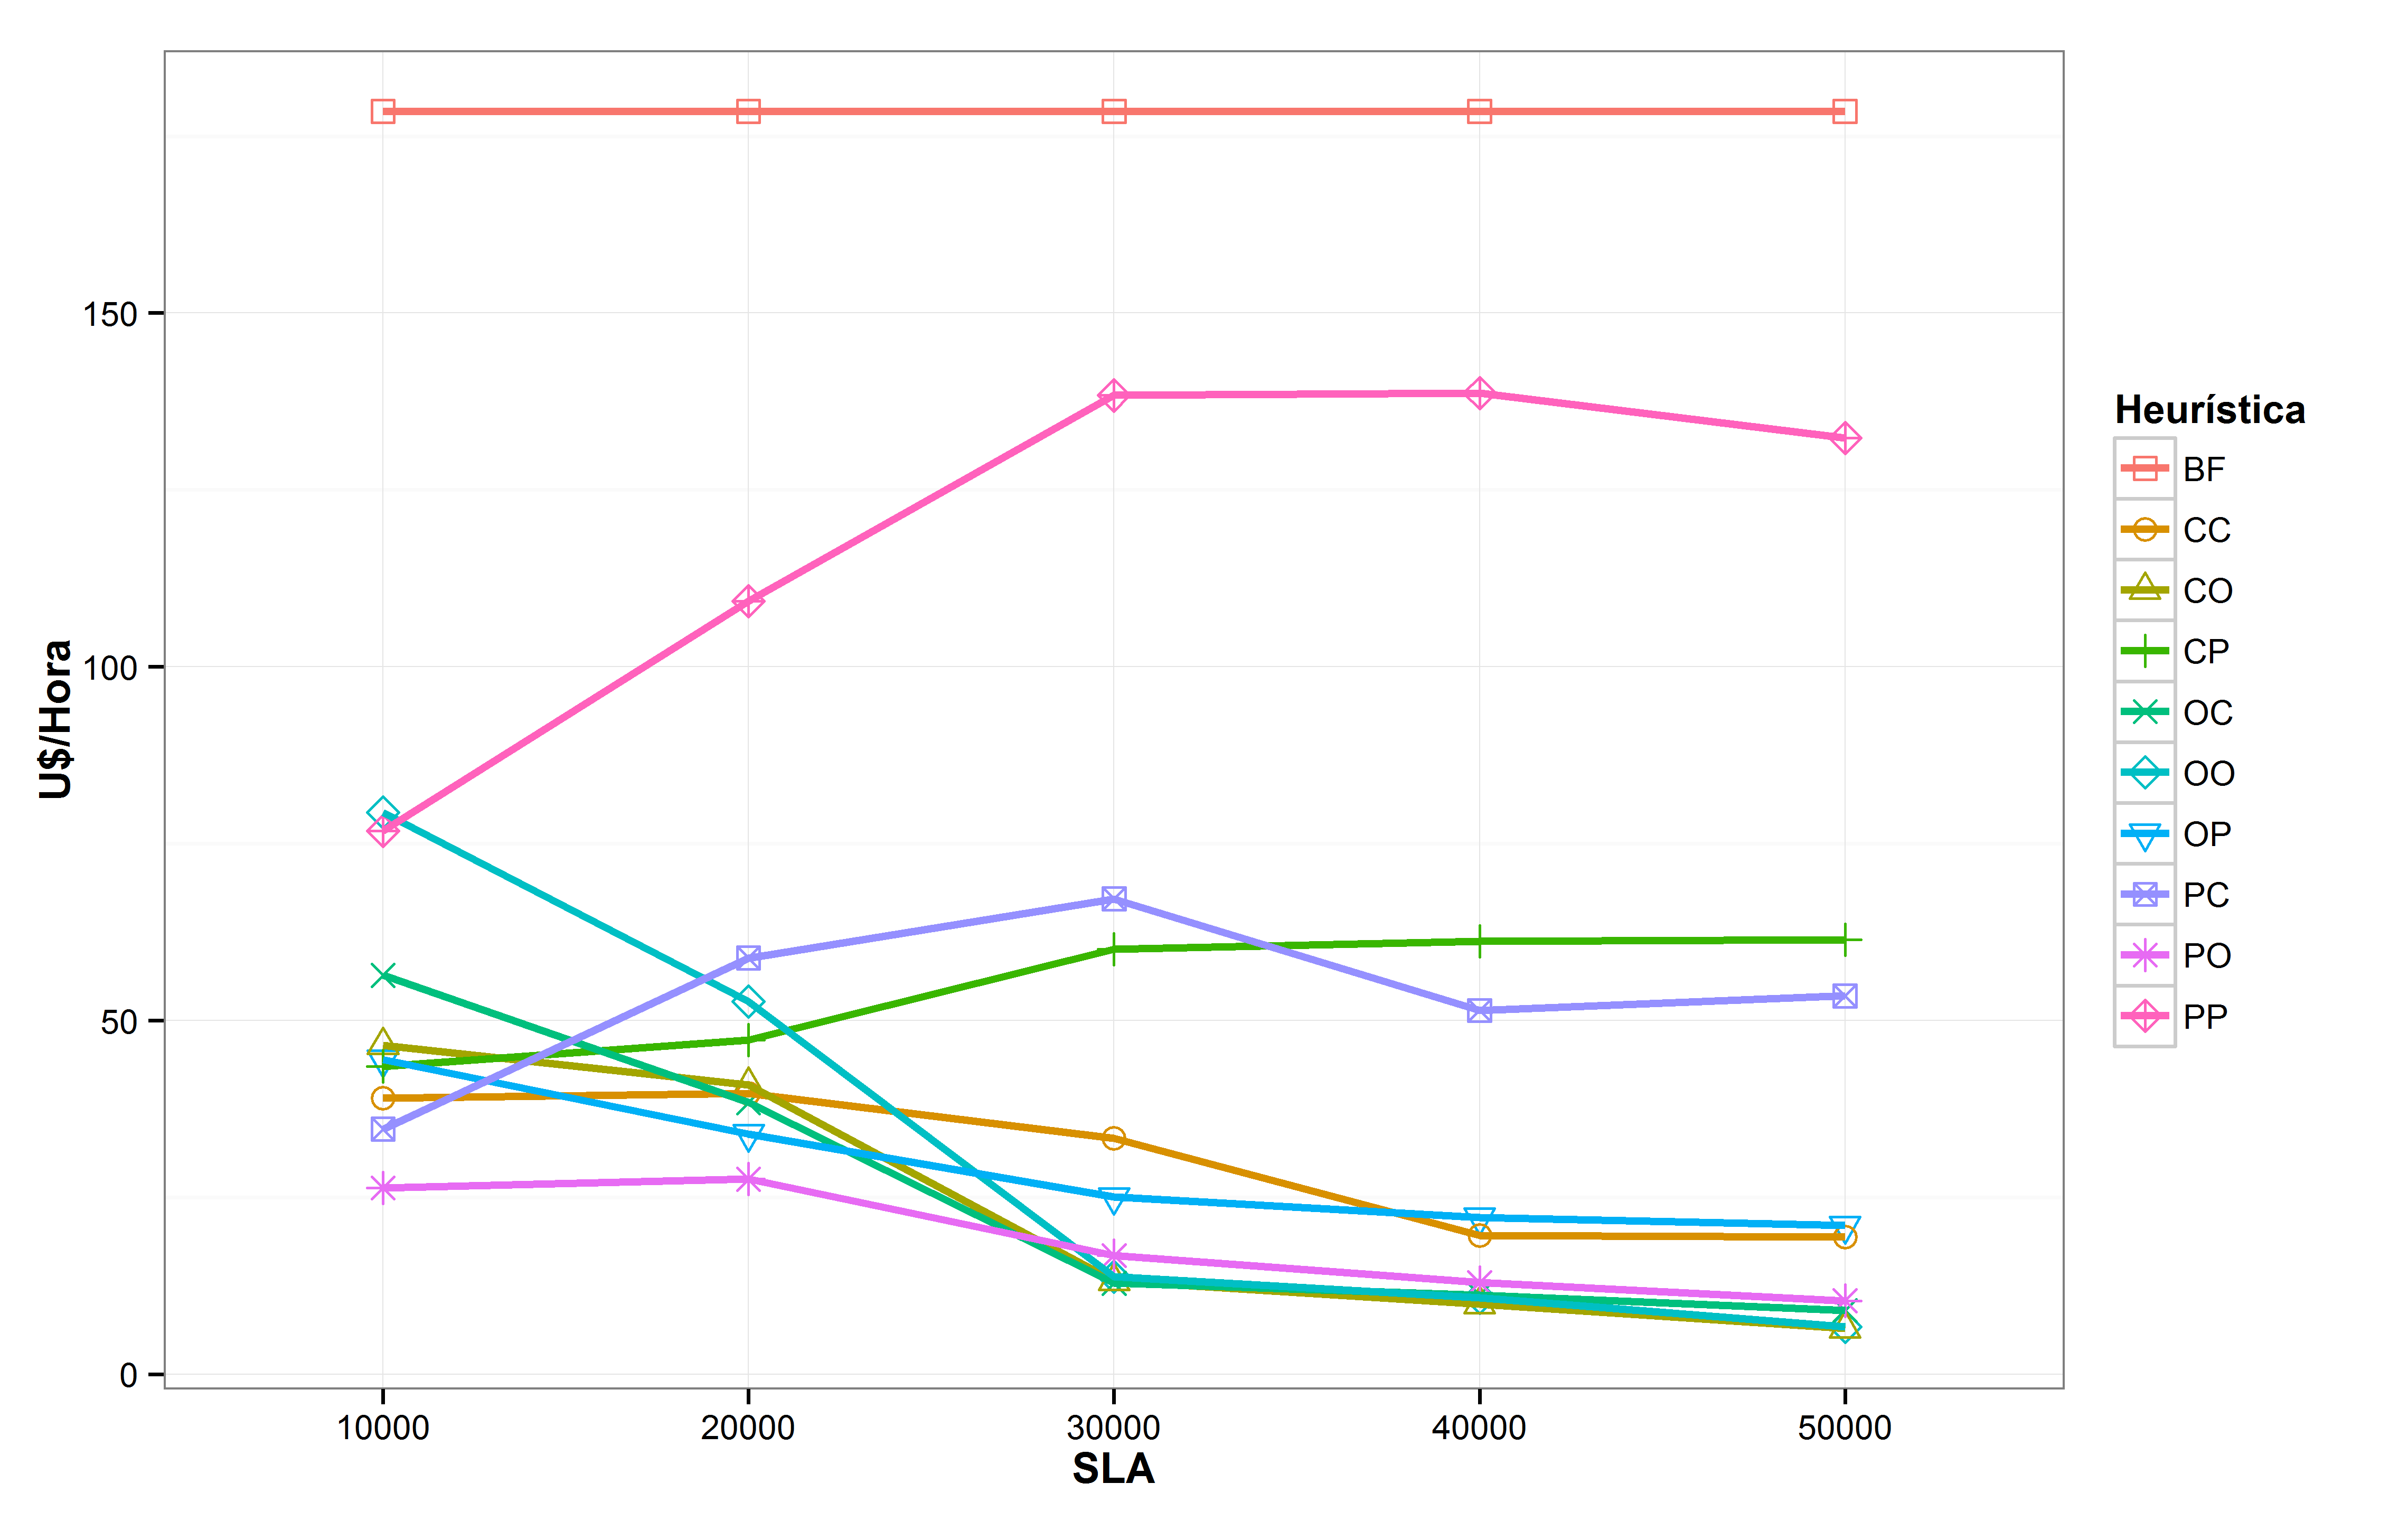
\includegraphics[width=\textwidth]{img/ExecutionCost-Capacity}
      \caption{Grafo por Capacidade}
      \label{fig:eficiencia_custo_capacidade}
    \end{subfigure}
    \begin{subfigure}[b]{0.7\textwidth}
      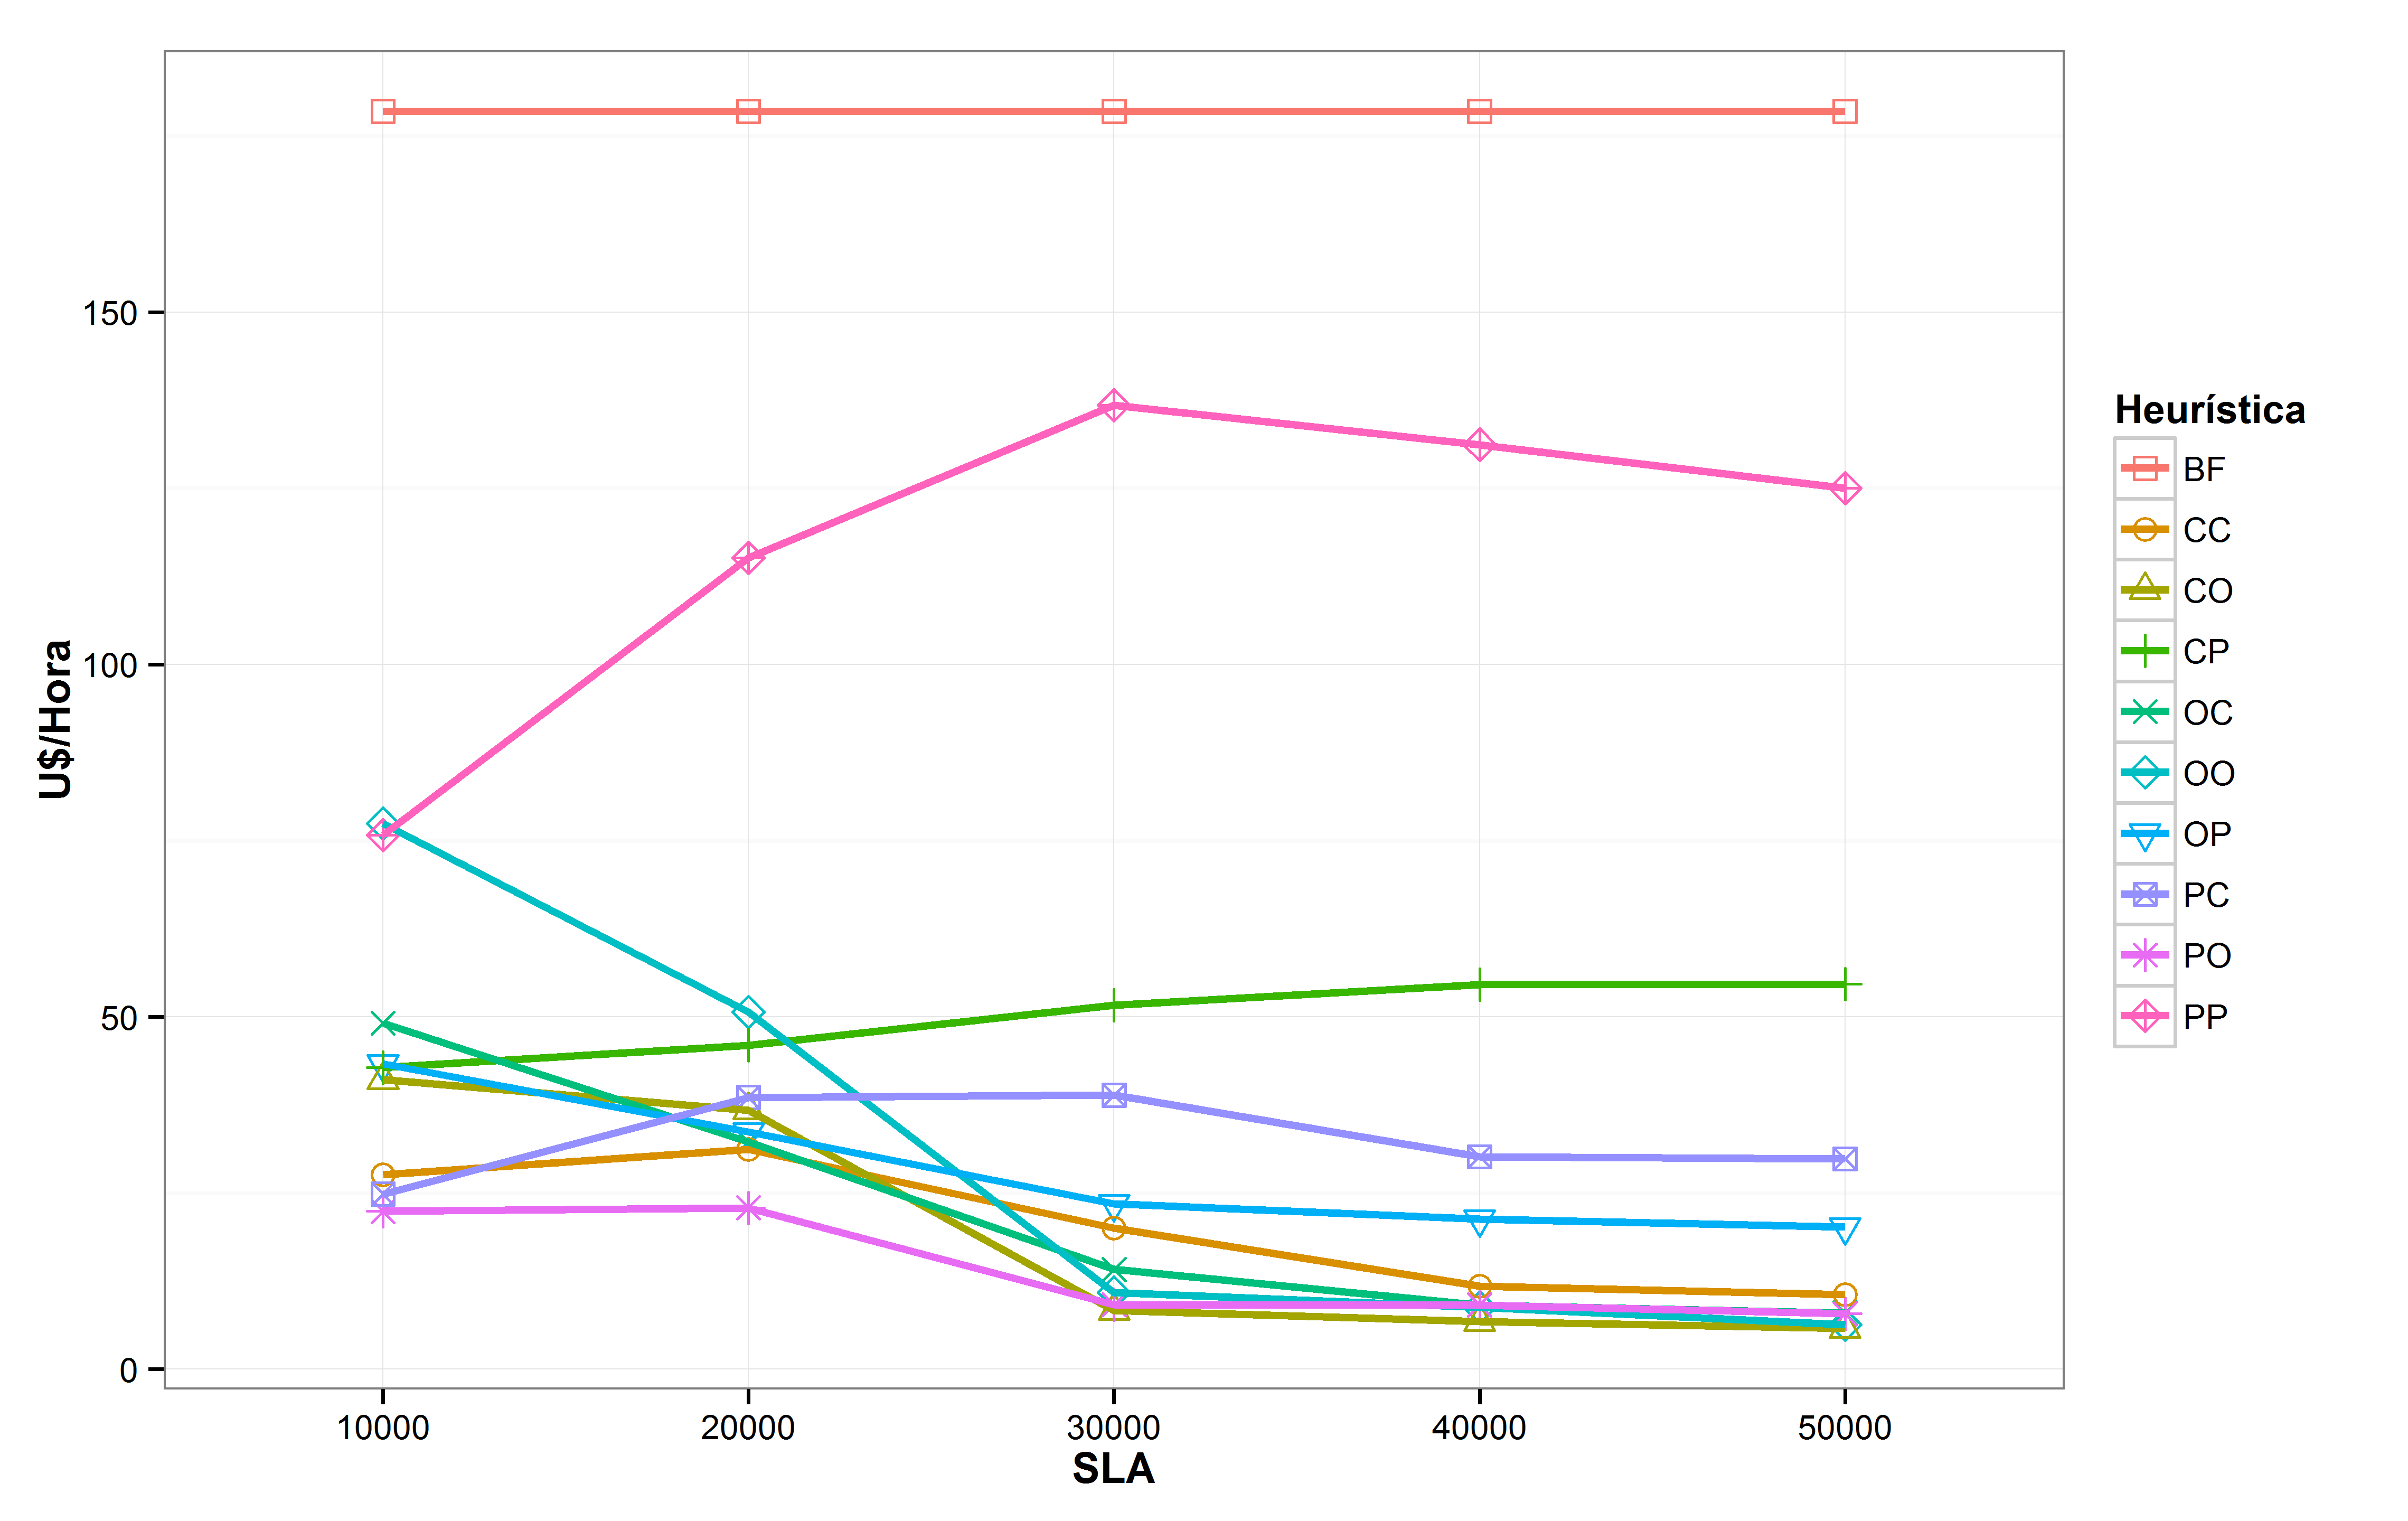
\includegraphics[width=\textwidth]{img/ExecutionCost-Price}
      \caption{Grafo por Preço}
      \label{fig:eficiencia_custo_preco}
    \end{subfigure}
  \caption{\label{fig:eficiencia_custo}Avaliação da Eficiência de Custo das Heurísticas}
\end{figure}

Para cada aspecto analisado, custo e número de execuções, foram realizadas duas 
baterias iguais de testes, uma utilizando o Espaço de Implantação gerado com base 
nas relações de poder computacional entre as Configurações e outra com o Espaço de 
Implantação baseado nas relações de preço. Essa variação foi feita para que fosse
possível estudar o efeito da regra de formação do Espaço de Implantação sobre o
desempenho geral do Processo de Inferência de Desempenho. Embora haja alguma 
diferença entre os resultados obtidos com ambas as representações, a percepção 
geral da eficiência das Heurísticas não muda.   

A Figura~\ref{fig:eficiencia_custo} mostra os gráficos dos resultados obtidos pelas
9 Heurísticas em termos de custo total dos testes de Avaliação considerando SLAs 
entre 10 e 50 segundos. O primeiro gráfico apresenta os resultados quando os testes
foram executados com a representação do Espaço de Implantação baseado na relação de
capacidade entre as Configurações. O segundo gráfico considera o grafo da relação
de preço das Configurações usado para representar o Espaço de Implantação.

\begin{figure}[hbt]
  \centering
    \begin{subfigure}[a]{0.7\textwidth}
      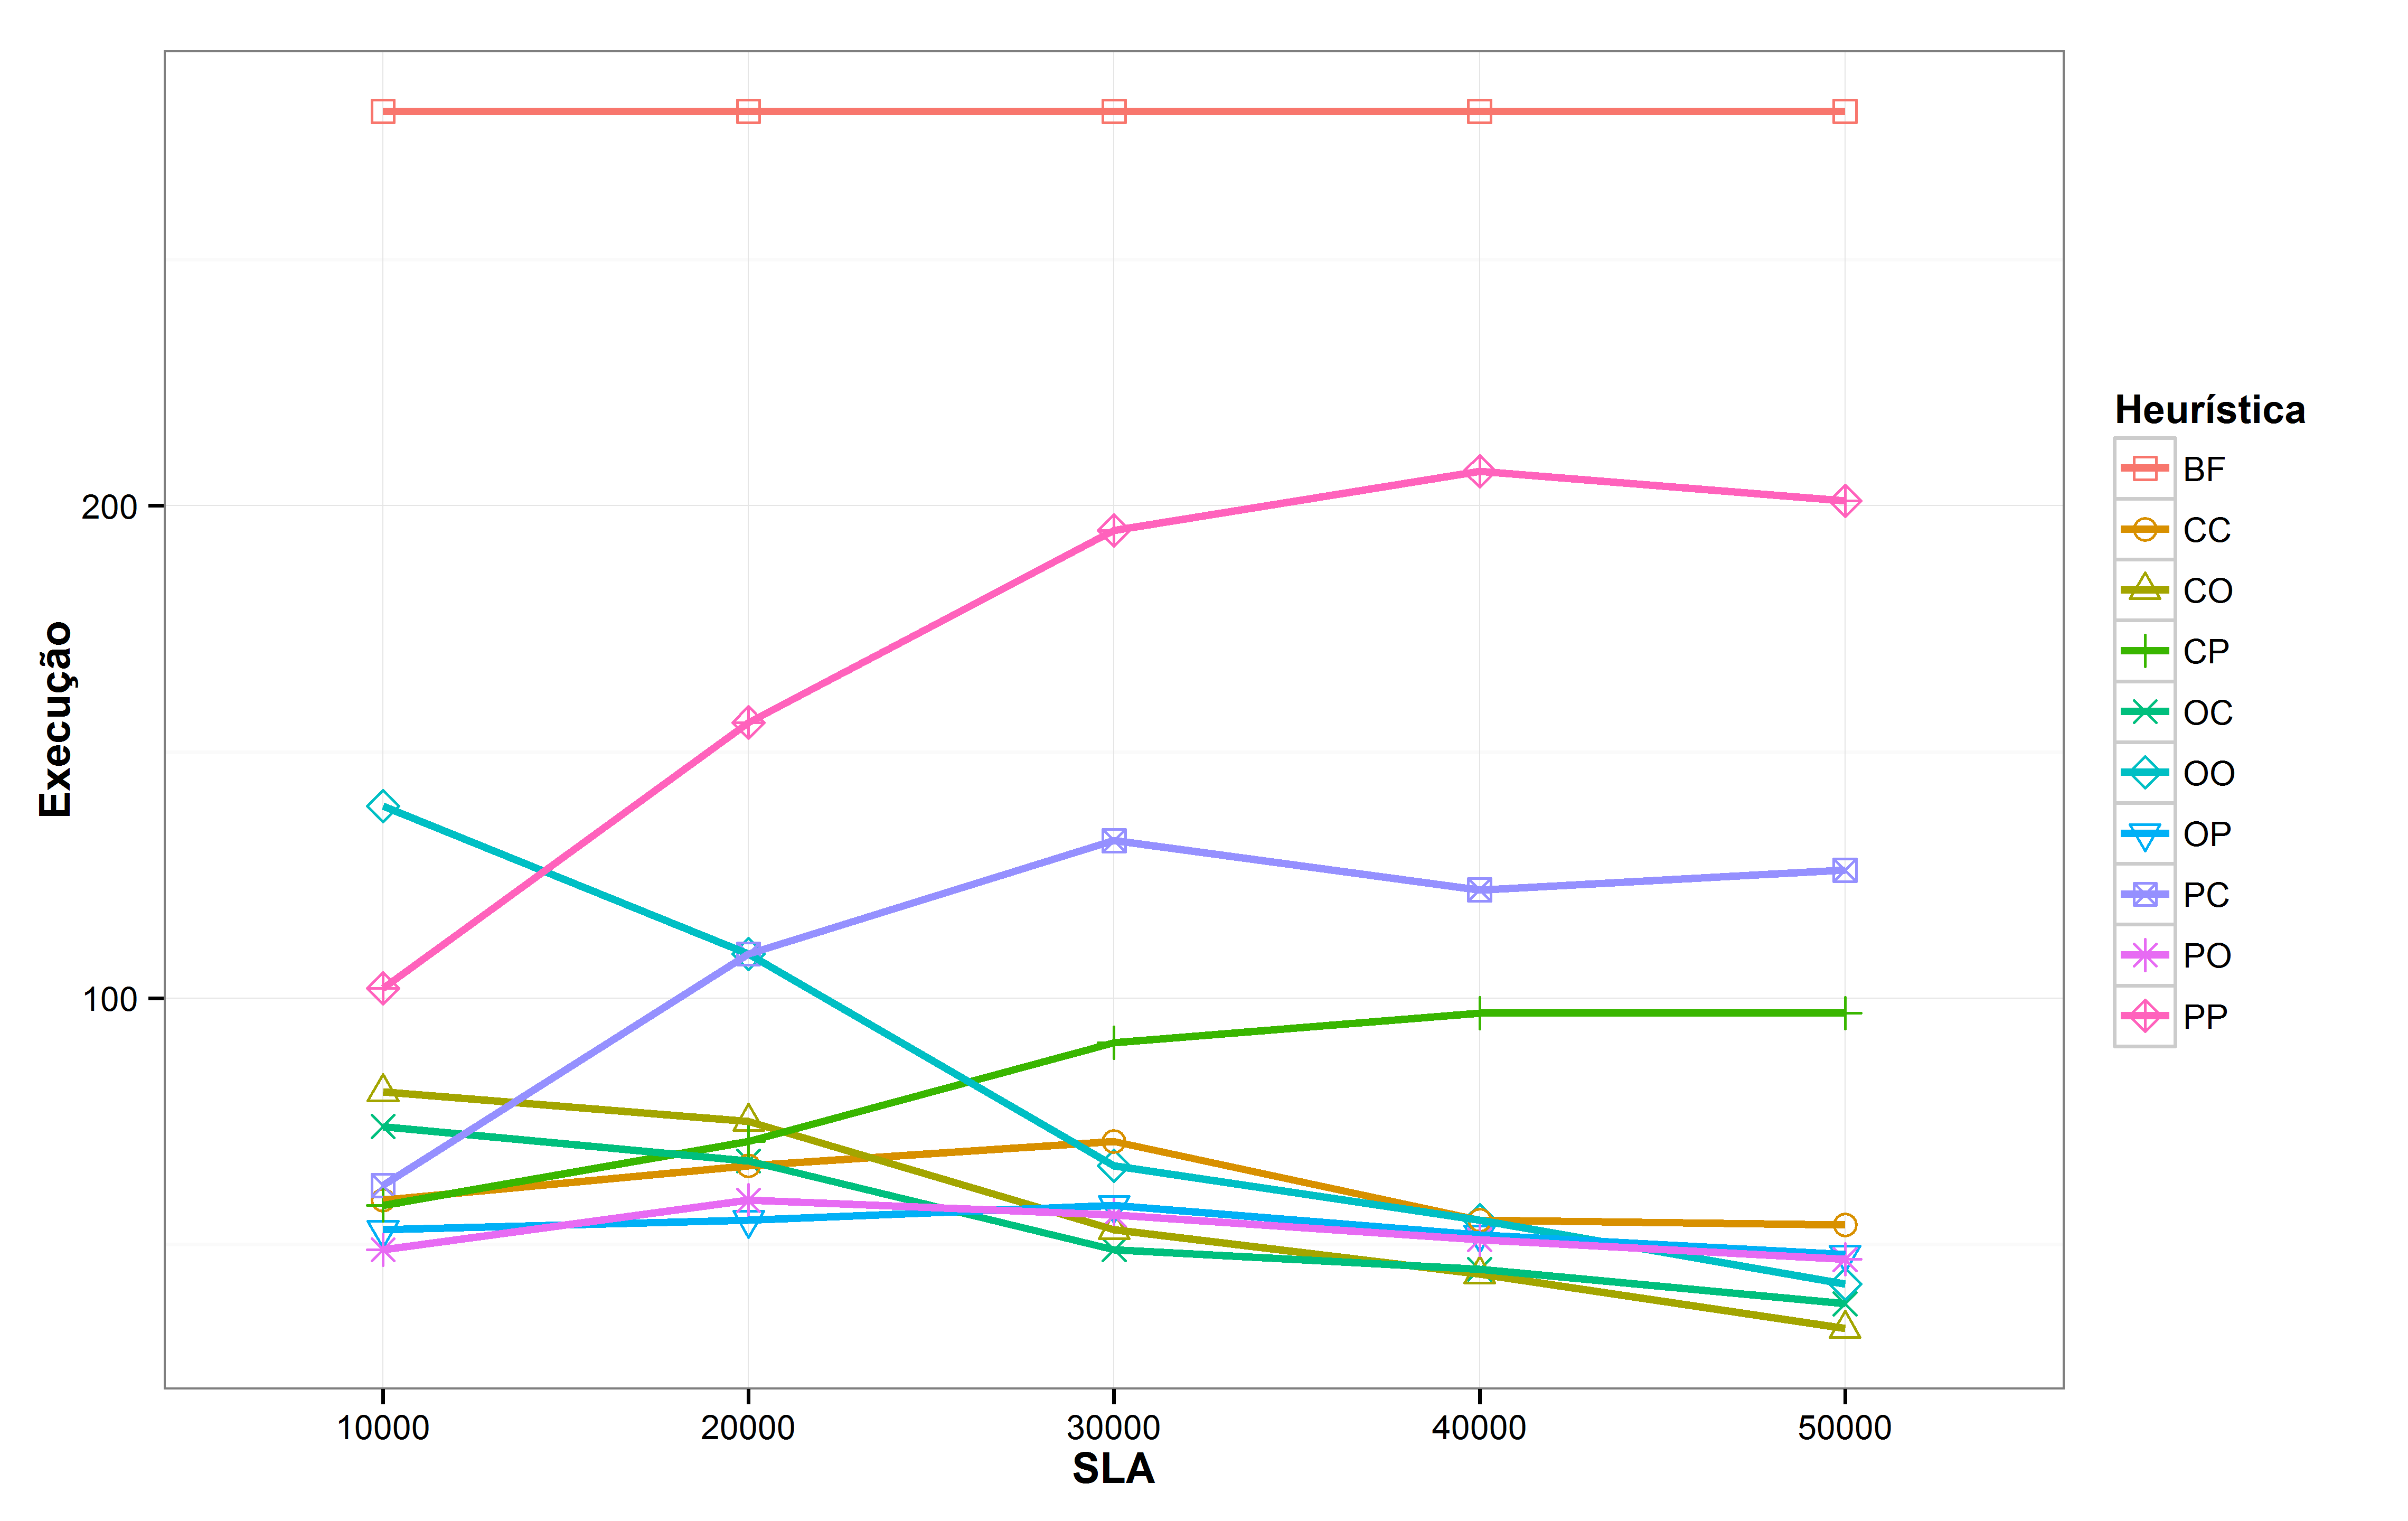
\includegraphics[width=\textwidth]{img/ExecutionCount-Capacity}
      \caption{Grafo por Capacidade}
      \label{fig:eficiencia_execucoes_capacidade}
    \end{subfigure}
    \begin{subfigure}[b]{0.7\textwidth}
      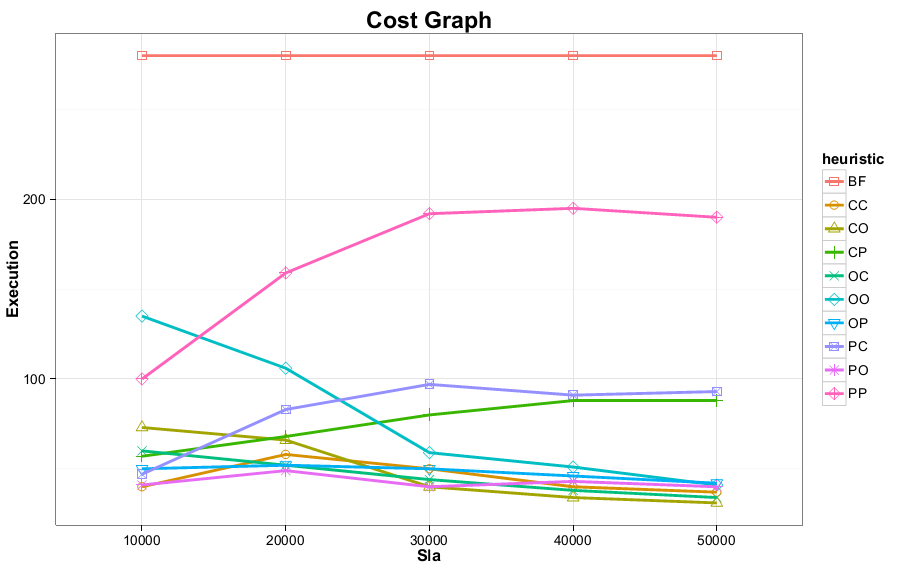
\includegraphics[width=\textwidth]{img/ExecutionCount-Price}
      \caption{Grafo por Preço}
      \label{fig:eficiencia_execucoes_preco}
    \end{subfigure}
  \caption{\label{fig:eficiencia_execucoes}Avaliação da Eficiência do Número de Execuções das Heurísticas}
\end{figure}

No topo de ambos os gráficos vê-se um linha horizontal que representa a 
\emph{baseline} de comparação, que é o custo total da Heurística de Força Bruta 
(\emph{Brute Force - BF}). Como o custo total para execução da Aplicação em todas
as combinações de Configurações e Cargas de Trabalho é sempre o mesmo, independente
do SLA requerido, a linha do gráfico para essa Heurística sempre é uma linha
horizontal.

A análise das imagens dos gráficos mostra que mesmo a Heurística com o pior 
desempenho no que se refere ao custo total da Avaliação já apresenta uma redução 
em relação à Força Bruta. Por outro lado, as melhores Heurísticas chegam a 
representar uma economia da ordem de 96\% em comparação com o que seria gasto
com a execução de todas as combinações de Configurações e Cargas de Trabalho.

Embora o comportamento das Heurísticas varie em função do SLA, é possível notar
que quando a exigência do SLA é mais moderada o comportamento de todas as Heurísticas
se estabiliza, tornando possível identificar que algumas delas tendem a
ser mais econômicas que as outras. Ainda que não seja possível afirmar que uma só 
Heurística seja a melhor em todas as situações, pode-se considerar que a Heurística
Pessimista~Otimista se mostra como a mais econômica em geral. A Heurística
Conservadora~Otimista merece atenção para os SLAs mais brandos, com os menores
custos absolutos nessas circunstâncias. 
 
A Figura~\ref{fig:eficiencia_execucoes} mostra o desempenho das Heurísticas sob 
o aspecto da quantidade de execuções reais da Aplicação sob Teste no ambiente de
nuvem alvo da Avaliação. Assim como a Figura~\ref{fig:eficiencia_custo}, essa 
imagem apresenta dois gráficos, que retratam o comportamento do Processo de 
Inferência ao usar as representações do Espaço de Implantação com grafos das 
relações de Capacidade e Preço entre as Configurações.

A análise desses gráficos faz notar um número de execuções até 88\% menor em 
relação à Heurística Força Bruta. Isso se reflete em menor tempo gasto no 
planejamento de capacidade e, consequentemente, menores custos, não só como já 
visto no que diz respeito à economia de horas de máquina, mas também de outros 
custos envolvidos em um projeto de software.

Tanto no aspecto custo como no aspecto quantidade de execuções, nota-se que a
Hedurística Pessimista~Pessimista tem um desempenho muito ruim, exigindo muitas
execuções e, por isso, elevando muito o custo do planejamento de capacidade. As
Heurísticas Pessimista~Conservadora e Conservadora~Pessimista ainda aparecem
um pouco descoladas do desempenho das outras Heurísticas, embora com uma redução
em torno de 65\% no número de execuções.

Os menores números de execuçõs são atingidos pelas Heurísticas Otimista~Conservadora 
e Conservadora~Otimista, sob os SLAs mais brandos. Porém, como não se saem tão 
bem sob SLAs mais rígidos, como 10 segundos, a Heurística Pessimista~Otimista
ganha destaque por ter comportamento mais estável, figurando entre as mais 
econômicas no aspecto de quantidade de execuções sob a maioria dos SLAs avaliados.
 
\section{Resumo}
Este capítulo descreveu os experimentos realizados neste trabalho como forma de
comprovar a hipótese de que é possível estabelecer uma relação de capacidade
entre as diversas configurações de máquinas usadas na implantação de uma aplicação
e, partindo dessa relação, é possível inferir o desempenho da aplicação em uma
configuração com base no desempenho observado em outra.

A execução de um sistema de avaliação desenvolvido com o uso da biblioteca 
CloudCapacitor, que implementa o Processo de Avaliação de Capacidade
por Inferência de Desempenho proposto no Capítulo~\ref{chap:processo}, demonstrou
que a Inferência de Desempenho é viável como técnica de suporte ao 
planejamento de capacidade, uma vez que a precisão de acertos das predições 
realizadas nos testes se aproxima muito dos 100\%.

Além disso, os experimentos mostram também que a aplicação do Processo de Inferência 
de Desempenho pode trazer até 96\% de economia financeira e até 88\% de economia 
de tempo na realização das atividades de testes de desempenho.

\begin{table}[htbp]
  \centering
    \begin{tabular}{|c|c|c|c|c|c|c|c|c|c|}
    \hline
    \multirow{2}{*}{Métricas} & \multicolumn{9}{c|}{Heurísticas} \\
    \cline{2-10}
                 & CC    & CO    & CP    & OC    & OO    & OP    & PC    & PO    & PP \\
    \hline
    Custo (US\$) & 25,23 & 21,55 & 52,31 & 24,05 & 31,74 & 28,85 & 42,79 & \cellcolor{OliveGreen}\textbf{\color{yellow}16,54} & 117,95 \\
    Tempo (h)    & 50,10 & 80,30 & 50,60 & 53,00 & 53,00 & 79,50 & 96,20 & \cellcolor{OliveGreen}\textbf{\color{yellow}47,50} & 169,70 \\
    Acurácia     & 0,997 & 0,998 & 0,997 & 0,997 & 0,998 & 0,997 & 0,997 & \cellcolor{OliveGreen}\textbf{\color{yellow}0,998} & 0,997  \\
    \hline
    \end{tabular}%
  \caption{\label{table:resultado_consolidado}Resultados Consolidados da Inferência de Desempenho}
  \label{tab:addlabel}%
\end{table}%

A Tabela~\ref{table:resultado_consolidado} apresenta uma consolidação geral dos
resultados obtidos por todas as Heurísticas definidas pelo Processo de Avaliação
de Capacidade por Inferência de Desempenho. Como pode ser observado, a Heurística 
Pessimista-Otimista atinge os melhores resultados, predizendo com uma precisão de 
99,8\% as melhores Configurações para executar a Aplicação sob Teste e gastando 
menos de US\$~17,00 e menos de 48 horas na média global para completar a Avaliação 
de Capacidade.  

Destacam-se ainda outras Heurísticas como Conservadora-Conservadora e 
Otimista-Conservadora, que, na média global, obtiveram resultados não muito acima
do atingido pela Pessimista-Otimista. A Heurística Pessimista-Pessimista, como
já mostrado na análise dos gráficos das 
Figuras~\ref{fig:eficiencia_custo}~e~\ref{fig:eficiencia_execucoes}, apresentou
resultados muito ruins quanto ao custo e ao tempo gastos para completar a Avaliação.

Esses dados consolidados comprovam ainda a grande precisão com que a predição
pela Inferência de Desempenho aponta as melhores Configurações para executar a
Aplicação sob Teste sob as mais variadas Cargas de Trabalho.
 



% ----------------------------------------------------------

% ----------------------------------------------------------

% ----------------------------------------------------------
% Conclusão
% ----------------------------------------------------------
\chapter{Conclusão}
\label{chap:conclusao}
% ----------------------------------------------------------
Este capítulo encerra este trabalho, apresentando uma síntese dos resultados 
obtidos, as contribuições e sugestões para trabalhos futuros.

\section{Resultados e Contribuições}
A oportunidade de adoção da computação em nuvem como alternativa para implantação 
de aplicações corporativas ante a expectativa de economia gerada pela tarifação 
sob demanda e a elasticidade de recursos traz consigo a necessidade de uma
avaliação prévia da viabilidade financeira da migração dessas aplicações para
o novo ambiente. Essa análise de viabilidade passa pela identificação de quais 
combinações de recursos entre os existentes na nuvem são potencialmente capazes 
de manter ou, preferencialmente, suplantar o desempenho original da aplicação em 
questão. Entre esses recursos, o de máquinas virtuais geralmente representam os
maiores custos de operação para aplicações implantadas na nuvem. Ao mesmo tempo,
é muito difícil prever qual será o custo operacional total na nuvem, exatamente
devido à característica de escalabilidade e elasticidade proporcionada pelo modelo
de implantação em nuvem IaaS.

Nesse contexto, este trabalho propôs uma nova abordagem para a pesquisa das 
melhores combinações de recursos de máquinas virtuais em provedores de nuvem IaaS.
A proposta se baseia no Processo de Inferência de Desempenho para Planejamento de
Capacidade, como descrito no Capítulo~\ref{chap:processo}. O Processo se apoia
na inferência de desempenho para determinadas configurações a partir da observação
do desempenho real de uma configuração ao executar de fato a aplicação no
ambiente de nuvem. A inferência é realizada pela interpretação do mapeamento das 
relações de capacidade existentes entre as diversas configurações que o provedor 
disponibiliza. A alta acurácia das inferências, acima de 99\% em média, conforme 
verificada pelos experimentos demonstrados no Capítulo~\ref{chap:resultados}, denota 
a confiabilidade das respostas dadas pela utilização do Processo de Inferência 
no apoio às atividades de planejamento de capacidade para migração de aplicações 
para o ambiente de nuvem. 

Paralelamente à confiabilidade, outro diferencial do Processo de Inferência é a 
economia financeira e operacional, em termos de tempo, na realização da fase de 
testes do planejamento de capacidade. Dado o enorme número de combinações de 
configurações possíveis entre recursos do Provedor, o uso de estratégias inteligentes,
com a aplicação das Heurísticas propostas para a seleção das combinações mais 
promissoras na busca pelas mais configurações mais baratas, confere ao Processo 
uma eficiência notável, destacada pela economia de até 96\% em custos e até 88\% 
em tempo de execução dos testes.  
  
\section{Sugestões para Trabalhos Futuros}
- realização de novos experimentos visando investigar até que ponto os resultados obtidos durante o mestrado podem ser generalizados para outras aplicações e provedores de nuvem;

- implementação e avaliação de novas heurísticas de inferência de desempenho, que levem em conta os dados de monitoramento dos recursos utilizados, incluindo memória, CPU e a distância do desempenho observado para o desempenho esperado (o "delta").

-  evolução do Capacitor para oferecer um serviço completo de implantação, avaliação e planejamento de capacidade de aplicações em nuvens IaaS.

% ----------------------------------------------------------

% ----------------------------------------------------------

% ----------------------------------------------------------
% ELEMENTOS PÓS-TEXTUAIS
% ----------------------------------------------------------
\postextual
% ----------------------------------------------------------

% ----------------------------------------------------------
% Referências bibliográficas
% ----------------------------------------------------------
\bibliography{dissertacao}

\end{document}
